\documentclass[]{book}
\usepackage{lmodern}
\usepackage{amssymb,amsmath}
\usepackage{ifxetex,ifluatex}
\usepackage{fixltx2e} % provides \textsubscript
\ifnum 0\ifxetex 1\fi\ifluatex 1\fi=0 % if pdftex
  \usepackage[T1]{fontenc}
  \usepackage[utf8]{inputenc}
\else % if luatex or xelatex
  \ifxetex
    \usepackage{mathspec}
  \else
    \usepackage{fontspec}
  \fi
  \defaultfontfeatures{Ligatures=TeX,Scale=MatchLowercase}
\fi
% use upquote if available, for straight quotes in verbatim environments
\IfFileExists{upquote.sty}{\usepackage{upquote}}{}
% use microtype if available
\IfFileExists{microtype.sty}{%
\usepackage{microtype}
\UseMicrotypeSet[protrusion]{basicmath} % disable protrusion for tt fonts
}{}
\usepackage[left=3cm,right=3cm,top=3cm,bottom=3cm]{geometry}
\usepackage{hyperref}
\hypersetup{unicode=true,
            pdftitle={Biostatistics in Public Health},
            pdfauthor={Ralph Trane},
            pdfborder={0 0 0},
            breaklinks=true}
\urlstyle{same}  % don't use monospace font for urls
\usepackage{natbib}
\bibliographystyle{apalike}
\usepackage{longtable,booktabs}
\usepackage{graphicx,grffile}
\makeatletter
\def\maxwidth{\ifdim\Gin@nat@width>\linewidth\linewidth\else\Gin@nat@width\fi}
\def\maxheight{\ifdim\Gin@nat@height>\textheight\textheight\else\Gin@nat@height\fi}
\makeatother
% Scale images if necessary, so that they will not overflow the page
% margins by default, and it is still possible to overwrite the defaults
% using explicit options in \includegraphics[width, height, ...]{}
\setkeys{Gin}{width=\maxwidth,height=\maxheight,keepaspectratio}
\IfFileExists{parskip.sty}{%
\usepackage{parskip}
}{% else
\setlength{\parindent}{0pt}
\setlength{\parskip}{6pt plus 2pt minus 1pt}
}
\setlength{\emergencystretch}{3em}  % prevent overfull lines
\providecommand{\tightlist}{%
  \setlength{\itemsep}{0pt}\setlength{\parskip}{0pt}}
\setcounter{secnumdepth}{5}
% Redefines (sub)paragraphs to behave more like sections
\ifx\paragraph\undefined\else
\let\oldparagraph\paragraph
\renewcommand{\paragraph}[1]{\oldparagraph{#1}\mbox{}}
\fi
\ifx\subparagraph\undefined\else
\let\oldsubparagraph\subparagraph
\renewcommand{\subparagraph}[1]{\oldsubparagraph{#1}\mbox{}}
\fi

%%% Use protect on footnotes to avoid problems with footnotes in titles
\let\rmarkdownfootnote\footnote%
\def\footnote{\protect\rmarkdownfootnote}

%%% Change title format to be more compact
\usepackage{titling}

% Create subtitle command for use in maketitle
\providecommand{\subtitle}[1]{
  \posttitle{
    \begin{center}\large#1\end{center}
    }
}

\setlength{\droptitle}{-2em}

  \title{Biostatistics in Public Health}
    \pretitle{\vspace{\droptitle}\centering\huge}
  \posttitle{\par}
    \author{Ralph Trane}
    \preauthor{\centering\large\emph}
  \postauthor{\par}
      \predate{\centering\large\emph}
  \postdate{\par}
    \date{Fall 2019(last compiled: 2019-10-08)}


\usepackage{amsthm}
\newtheorem{theorem}{Theorem}[chapter]
\newtheorem{lemma}{Lemma}[chapter]
\newtheorem{corollary}{Corollary}[chapter]
\newtheorem{proposition}{Proposition}[chapter]
\newtheorem{conjecture}{Conjecture}[chapter]
\theoremstyle{definition}
\newtheorem{definition}{Definition}[chapter]
\theoremstyle{definition}
\newtheorem{example}{Example}[chapter]
\theoremstyle{definition}
\newtheorem{exercise}{Exercise}[chapter]
\theoremstyle{remark}
\newtheorem*{remark}{Remark}
\newtheorem*{solution}{Solution}
\let\BeginKnitrBlock\begin \let\EndKnitrBlock\end
\begin{document}
\maketitle

{
\setcounter{tocdepth}{1}
\tableofcontents
}
\hypertarget{introduction-to-notes}{%
\chapter{Introduction to Notes}\label{introduction-to-notes}}

\newcommand{\Var}{\text{Var}}
\newcommand{\var}{\text{var}}
\newcommand{\SD}{\text{SD}}

Welcome to Public Health 783. This is where you'll find my notes for the biostatistics part of this class for Fall 2019.

These notes are meant to be a supplement to lectures and \citet{ls}. If you have any doubts as to what parts of the book I think are more important, this is a good place to look. There's a good chance that if it is not included here, I do not care too much about it. That being said, things included here might not be elaborated to a satisfying extent, and therefore I do \emph{NOT} recommend that you rely solely on these notes, but rather use them in conjunction with the book, and, just as importantly, lectures.

I want to emphasize that these notes are not exhaustive, but are meant to complement lectures. We simply won't have time to cover everything in the amount of detail I would like. Therefore, I will use these notes to write down some thoughts on certain topics that I think you might as well read outside the classroom. At times I will ask you to read sections before showing up to lectures. Other times, I won't even make the material available to you until after lectures. There's good reason for that. Some things are easier to explain when you have already seen them before. Other concepts can be scary on paper, and are best introduced by another human being. In either case, it is extremely important that you show up to lectures.

Finally, note that this collection is a living thing. It will change throughout the semester as we move along. Sometimes I might go back and clarify sections, if it seems to be necessary. At the beginning of the class you'll only find the first part, but as we make our way through, I will publish more notes on the topics to be covered later.

\hypertarget{bounty-program}{%
\section*{Bounty Program}\label{bounty-program}}
\addcontentsline{toc}{section}{Bounty Program}

As already mentioned, this is a living document. Furthermore, it is very much so the first version. Therefore, there will inevitably be mistakes. Hopefully, most of them will be minor, but I would be surprised if there isn't a few major ones here and there. Therefore, I really hope that you will all help me out and let me know whenever you find mistakes, no matter how small they might seem.

Now, I know that noone wants to do that -- who has the time to send an email just to let some fool know they can't spell ``stastitics''. But it's important to me to gradually improve these notes, and often being made aware of small mistakes opens up ones eyes to bigger ones. So to incentivize you to report mistakes, I have decided to start a bounty program: if you as a group gather more than 20 points (see below on how to collect points), there will be a reward at the end of the semester! If you find a mistake, simply shoot me an \href{mailto:rtrane@wisc.edu}{email}, let me know where the mistake is, and what type you think it is.

\begin{longtable}[]{@{}ll@{}}
\toprule
Type of Mistake & Points\tabularnewline
\midrule
\endhead
Spelling/grammatical error & 1\tabularnewline
Math error & 2\tabularnewline
Conceptual nonsense in either text or math & 3\tabularnewline
\bottomrule
\end{longtable}

\hypertarget{intro}{%
\chapter{Introduction to Biostatistics}\label{intro}}

\hypertarget{what-is-biostatistics}{%
\section{What is Biostatistics?}\label{what-is-biostatistics}}

Biostatistics is ``simply'' statistics applied to a specific set of problems, namely problems related to biological questions. Hence, the question ``what is biostatistics?'' is quickly replaced by ``what is statistics?''

From Wikipedia\footnote{\ldots{} because where else do you go when you're not sure where to start?}: ``Statistics is the discipline that concerns the collection, organization, displaying, analysis, interpretation, and presentation of data.'' That is quite the range, but all it is saying is that statistics is the science of making sense of data.

It is very hard to pinpoint exactly what statistics is, but it is rather easy to dismiss at least one very common misunderstanding: statistics is \emph{NOT} an exact science. There is (almost) never just one answer to a question. Rather, statistics is a decision science in the sense that at every step of the way, from study design to data collection to data presentation to data analysis and interpretation, you have to make decisions. And inevitably, your conclusions depend on every single one of those decisions.

\hypertarget{biostatistics-in-publhlth-783}{%
\section{Biostatistics in PUBLHLTH 783}\label{biostatistics-in-publhlth-783}}

In this class, we'll be considering what might seem like a very simple setup with simple questions, and a general approach to answering said questions. The truth is basically all statistical methods, no matter how complicated they might seem, follow (to some extend) this exact pattern. In this class, we will work our way through this pattern, and talk about how the simplest of methods work. The hope is that when we're done, you take these simple methods with you, and whenever you encounter more complicated methods, you can draw parallels back to what you have seen here, which hopefully will help you make at least some sense of even the most complicated methods.

The story begins\ldots{}

Any statistical analysis begins with a research question. This question always relates to a certain \emph{feature} or \emph{characteristic} of a certain \emph{population}, or of multiple populations. The population is the group of entities one wants to learn more about. It could be that one is interested in the life expectancy (feature) of U.S. adults (population), risk of diabetes (feature) among people with a certain genetic profile (population), the resistance to a disease (feature) among ants in Governor Dodge State Park (population), strength (feature) of pipes produced by a certain manufacturer (population), etc.

Now, the first fundamental idea of the approach we'll pursue in this class is this: there is a single true answer to the question asked. The only one way to obtain the truth is to observe the entire population. If we could measure the disease status (diabetes/no diabetes) of every single individual with the genetic profile of interest, we could evaluate the true risk. The catch is, maybe obviously to someone, that this is simply not feasible. Often we do not even know exactly how big the population of interest is, which means it is impossible to survey every single subject in the population. And even if we knew exactly how many people were part of the population, how to get a hold of them, and how to convince them to participate in our study, it is very unlikely we would have the resources (read: \$\$\$) to reach out and include every single one of them.

This leads us to the picture we will return to over and over again in this class: there is some population of interest. We want to say something about a certain feature of the population. This will usually be a mean of a measurement, the risk ratio or odds ratio of two groups, or something similar. Unfortunately, there is no way we can actually measure the feature for every single subject in the population -- if we could, we would simply calculate the mean, and be done with it! Instead, we take a \emph{sample} from the population. The hope is that we obtain this sample in such a way that the sample is representative of the entire population, and therefore we can use the information obtained from the sample to say something about the population.

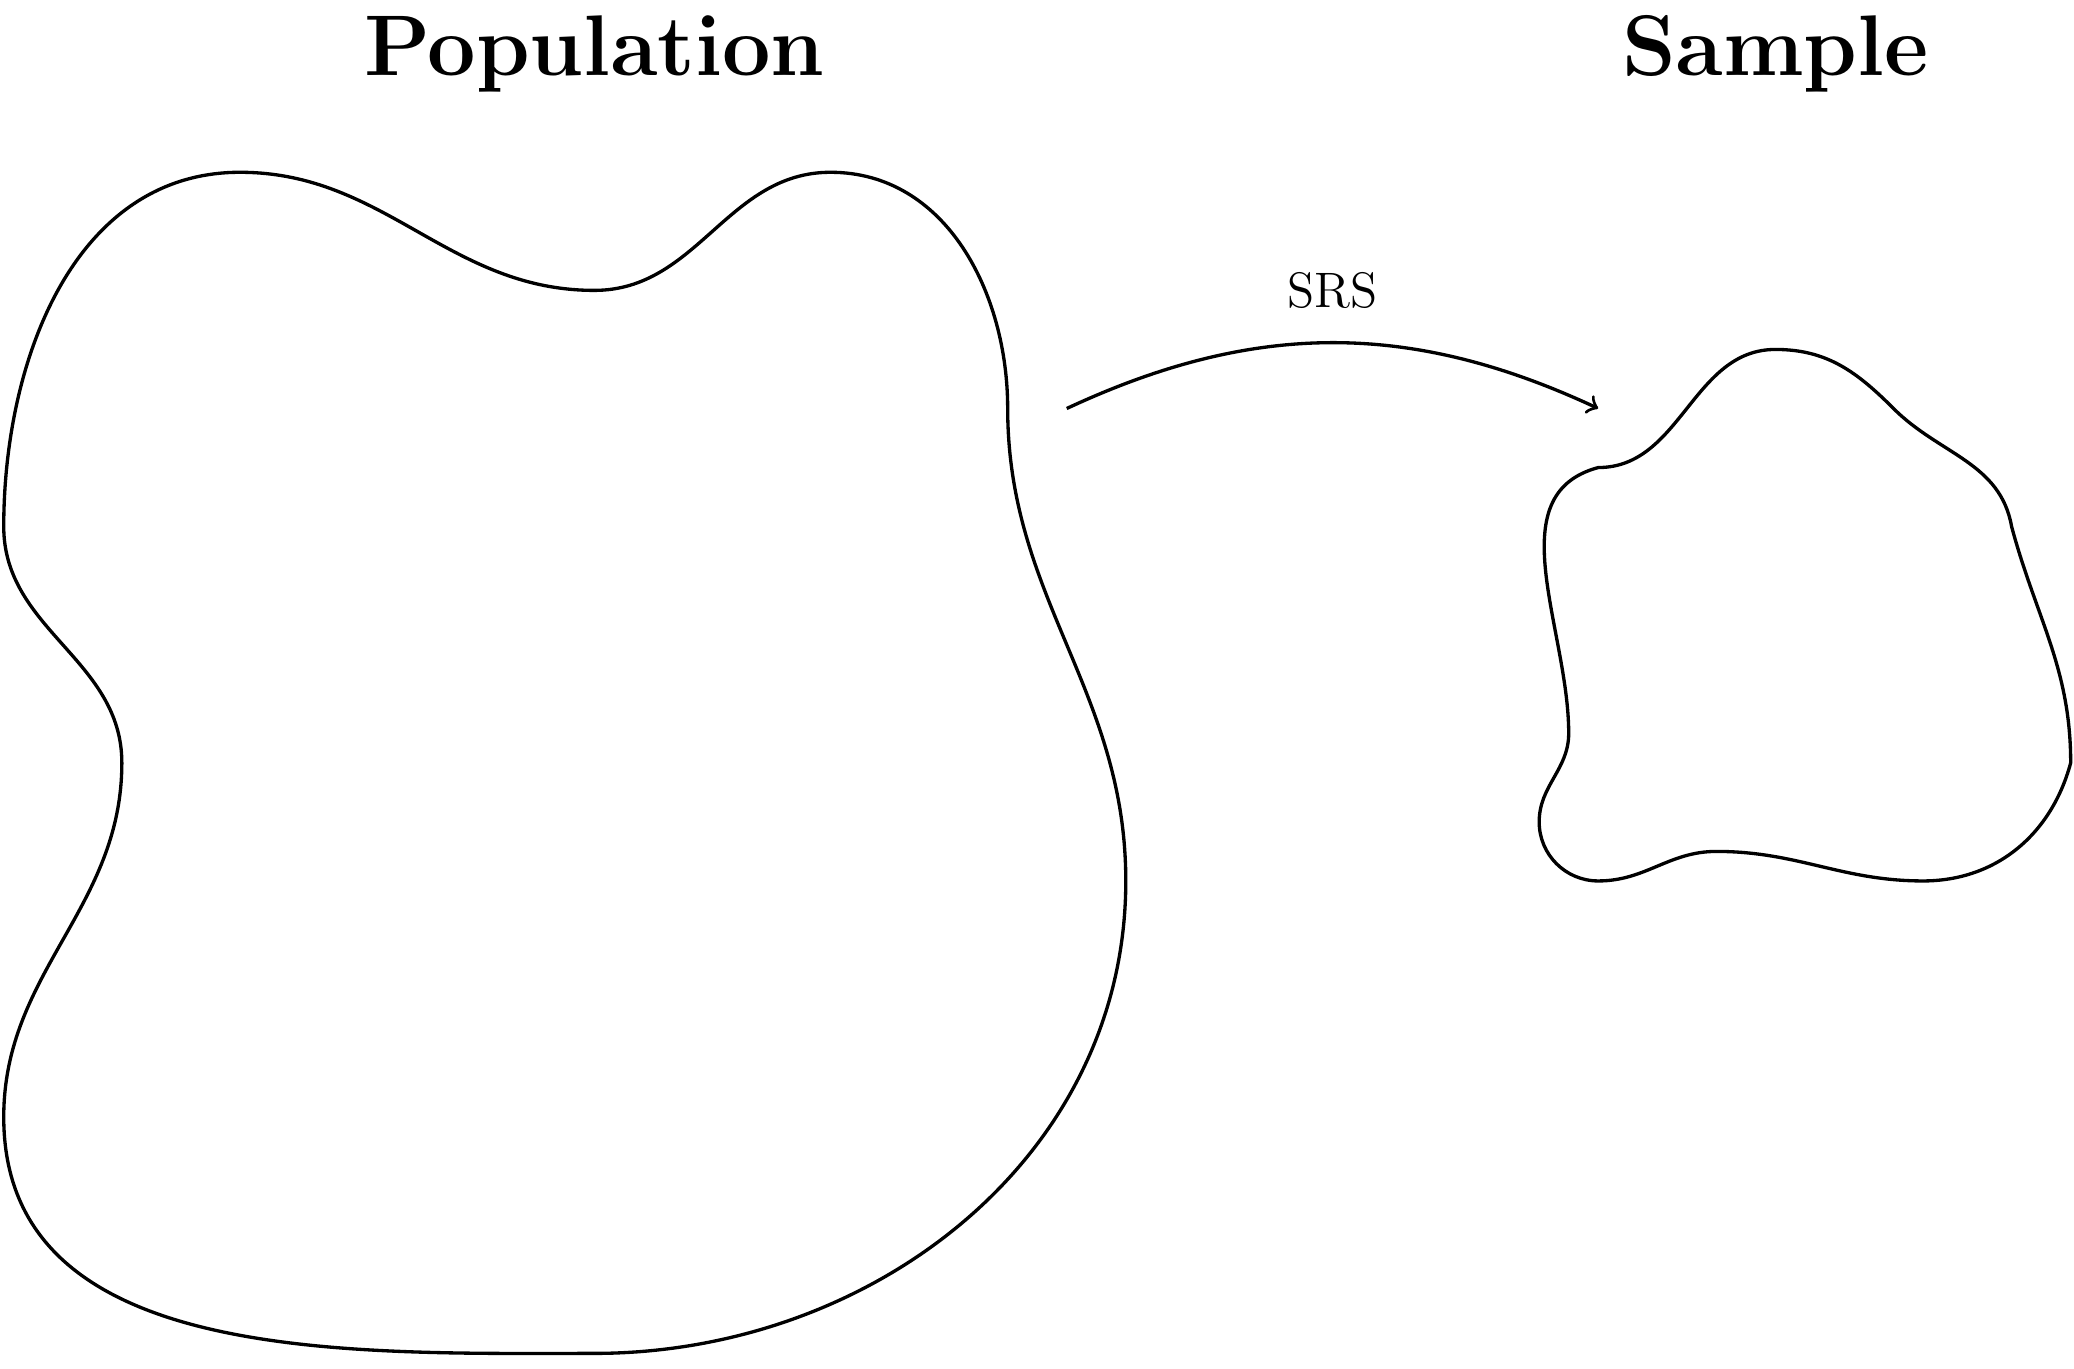
\includegraphics{783_biostats_files/figure-latex/unnamed-chunk-3-1.pdf}

When we talk about chances of observing something when sampling from the population, we talk about \emph{probabilities}. What is the probability a sample of 23 people has more than 5 diabetics? What is the probability a randomly chosen individual from Minneapolis will develop cancer?

When we try to use a sample to say something about the general population from which the sample was created, we do \emph{inference}.

The plot thickens\ldots{}

We now have an idea of what it is we want to do: take a sample, obtain some information about the thing of interest, then use that information to say something about the general population. Pretty simple. The problem is, how do we actually put the pieces together in a way that allows us to generalize to the population? Example: we are interested in estimating the prevalence of cardiovascular disease in the general population of U.S. adults. We have a hunch that the true prevalence is 11\%. We take a sample of 3799 female U.S. adults of which 379 have a history of CVD. So, the prevalence is estimated to be \(\frac{379}{3799} \approx 10 \%\)\footnote{This data was obtained from the Framingham Offspring Study, see table 3-1, page 24 of \citet{ls}}. The prevalence in our sample is clearly different from our hypothesis, so clearly our hypothesis is wrong\ldots. right?

If only it was that simple. The problem here is that our prevalence estimate depends on the specific sample we got. If we were to repeat this experiment, we would ask a different group of people about their history of CVD, which would lead to a different estimate of the prevalence. There's simply no way (or it is at least very, very unlikely) we'll ever get a sample of people for which the prevalence matches our hypothesis exactly. So the question is not simply if our sample has the same prevalence as hypothesized, but rather is it ``close enough'' for us to believe our hypothesis.

Close enough? Did I read that right?

Yup. The majority of statistical methods, and definitely everything we'll be talking about in this class, are trying to decide if what we observe in our sample is ``close enough'' to our hypothesize about the population. The idea is that if what we observe is very far from our hypothesis, then it is unlikely that the hypothesis is true.

There are generally two ways of framing the question:

\begin{enumerate}
\def\labelenumi{\arabic{enumi}.}
\tightlist
\item
  Is what we observe (think prevalence in sample) ``close enough'' to the hypothesis (that the prevalence in the population is 11\%)?
\item
  What range of hypotheses (values for the prevalence) would we accept given what we observed?
\end{enumerate}

The first approach is refered to as testing a \emph{statistical hypothesis}, or \emph{null hypothesis significance testing} (NHST), while the second is refered to as constructing a \emph{confidence interval}. These two are closely related, as we will see later, but the information contained in the results differ drastically. While testing a hypothesis only provides you with a result concerning \textbf{one value}, the confidence interval gives you a wide range of values that you to some extent believe could be the true value. Why would anyone then ever report the result of a statistical hypothesis test without a confidence interval, you ask? That is a very, very, very good question to which I do not have an answer\ldots{}

This has all been very abstract (and I think I got carried away in that last paragraph). We'll see examples of this over and over again throughout the semester, so hopefully it'll be easier to comprehend as we go along.

\hypertarget{part-data-types-and-descriptive-statistics}{%
\part{Data Types and Descriptive Statistics}\label{part-data-types-and-descriptive-statistics}}

\hypertarget{before-we-get-started}{%
\chapter{Before we get started\ldots{}}\label{before-we-get-started}}

This section is very minimal. I decided to go that route because 1) this is the ``easiest'' part of the material in the sense that there isn't a lot of things to really understand and think about, and 2) it is objectively speaking very, very, very boring\ldots{} So, when you find my notes insufficient, take a look at Chapter 4 in \citep{ls}.

\textbf{Learning Objectives}

\begin{enumerate}
\def\labelenumi{\arabic{enumi}.}
\item
  Understand why descriptive statistics is important, and useful
\item
  Know the difference between discrete and continuous variables/data
\item
  Have some ideas of which summaries and figures are appropriate for different types of data
\end{enumerate}

\hypertarget{why-descriptive-statistics}{%
\chapter{Why Descriptive Statistics?}\label{why-descriptive-statistics}}

\emph{Descriptive Statistics}, as the name implies, are about describing something. In general, we can only describe what we have at hand, so descriptive statistics only deal with the population in the very, very, very rare case when we have measured the entire population. It is way more common that descriptive statistics are about the sample at hand.

Often when conducting an experiment, what we are actually interested in is using the sample we obtain to say something about the general population. If we, for example, enroll 200 patients in a study to find out if a new drug works, we're not \emph{really} interested in whether or not it works for those 200 patients specifically, but more so if it works for any individual from the population in general. With that in mind, the whole concept of descriptive statistics might not seem very (1) exciting, (2) useful, or (3) necessary. While (1) is highly subjective, (2) very much so depends on the specific situation, there is little question that it is in fact necessary.

Recall our general setup for any statistical analysis: we have some question about some feature of a population. To answer this question, we go get a sample of the population. If this is a good sample, the characteristics of this sample mimic those of the general population. If this is the case, then the hope is that we can draw conclusions about the sample, and generalize them to the general population. Conversely, if that is \emph{not} the case, then no matter how convincing the evidence we find in the sample is for or against our hypotheses, it tells us nothing about the general population.

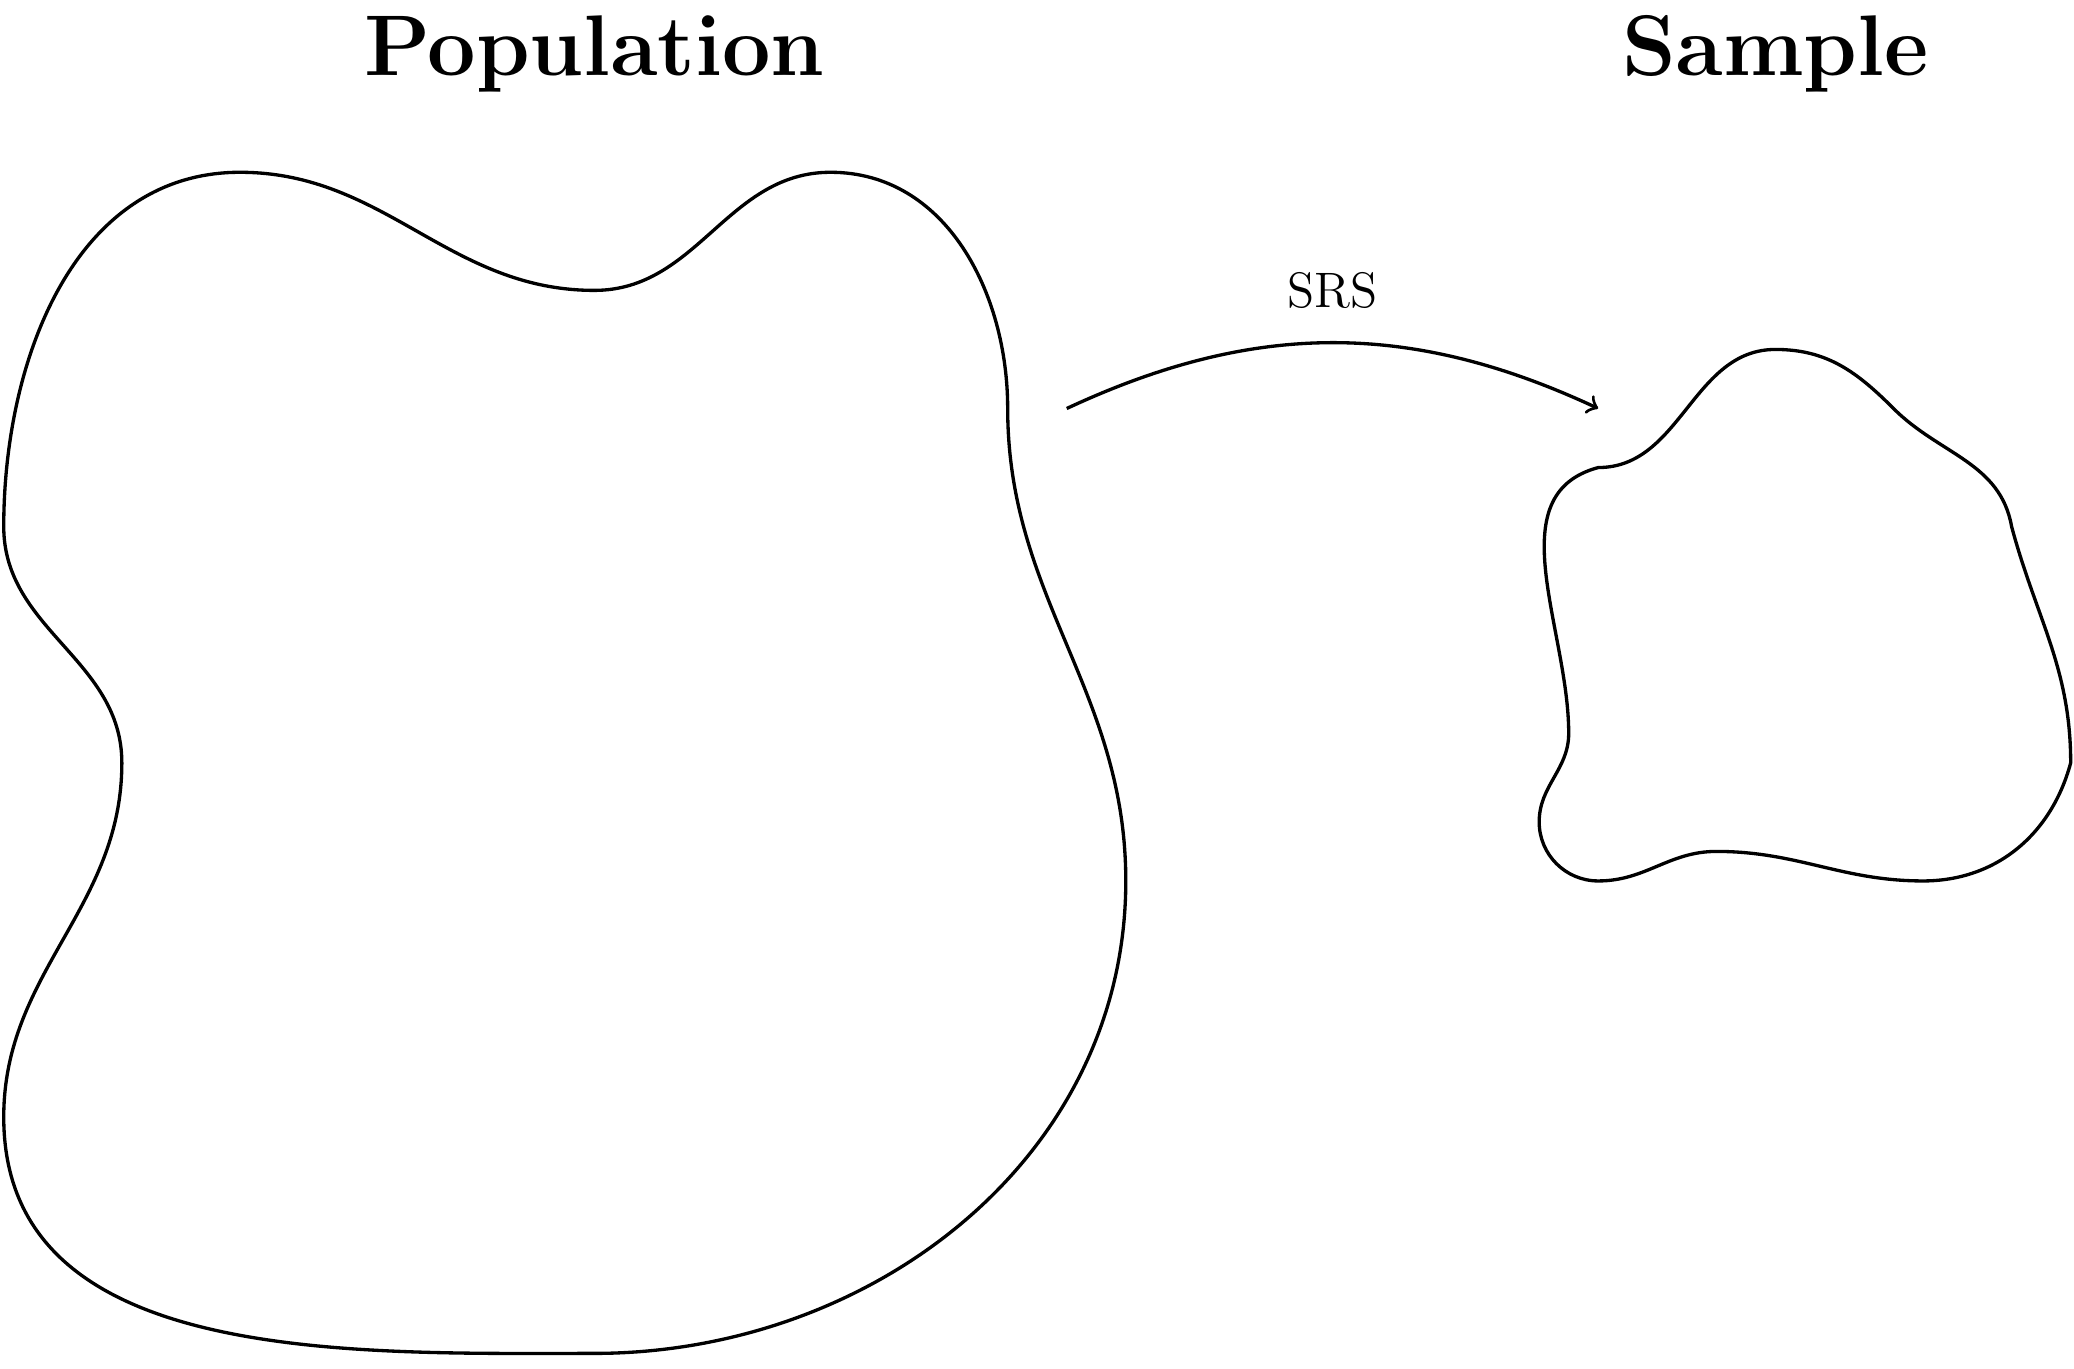
\includegraphics{783_biostats_files/figure-latex/general-population-1.pdf}

So how do we make sure the sample is representative of the population? The first step is to make sure our sampling scheme is good. Ideally, we sample completely at random, meaning that every single individual in the population has the same chance of ending up in the sample. As you might be able to guess, this is rarely the case, but if the sampling is done right it is either approximately true, or the sampling is done in a way that any biases introduced can be accounted for in the analysis.\footnote{\textbf{Full disclaimer}: sampling is hard. As in really, really, really hard. Very smart people spend a lot of time on making sure different sampling schemes work. It is well beyond the scope of this course, and me, how the details of this work out.} Most commonly, sampling is done in such a way that the ``equal chance'' assumption isn't too crazy. But how do we know if this is actually the case?

The truth is, we don't really. What we can do, though, is describe the sample we obtain. That way we can make sure we don't generalize any results to an inappropriate population. Historically, this mistake has been made over and over again in medical research when excluding women and ethnic minorities from studies.\footnote{See \citet{liu_womens_2016} for a more thorough discussion of the exclusion of women in particular.} For this particular reason, producing descriptive statistics is often the first step in any data analysis.

The rest of this section will go through different types of data, and show how we, in each case, can describe (or summarize, if you will) the specific type of data.

In general, when we talk about data we often refer to \emph{variables}. Variables are simply (and very vaguely) \emph{things we measure}. You will see examples which hopefully helps understand exactly what is meant by a variable.

\hypertarget{discrete}{%
\chapter{Discrete Data}\label{discrete}}

A variable is called a \emph{discrete} variable if the possible values of the variable are countable, that is if you can count them. Note that a discrete variable can technically have an infinite number of possible outcomes.

A discrete variable is of one of two subtypes: \emph{categorical} or \emph{ordinal}.

\hypertarget{categorical}{%
\section{Categorical data}\label{categorical}}

Categorical variables are discrete variables with no particular ordering of the categories.

\hypertarget{examples-categorical-data}{%
\subsection{Examples -- categorical data}\label{examples-categorical-data}}

The classical example of a categorical variable is sex. For each subject, the value of this variable is one of two possible values: male or female.

Other examples:

\begin{itemize}
\tightlist
\item
  color
\item
  race
\item
  blood type
\item
  country of origin
\item
  political orientation
\end{itemize}

\hypertarget{binarydichotomous-data}{%
\subsection{Binary/Dichotomous Data}\label{binarydichotomous-data}}

Often researchers will refer to certain variables as \emph{binary} or \emph{dichotomous}. This simply means \emph{categorical with two categories}.

\hypertarget{how-to-describe-categorical-data}{%
\section{How to describe categorical data}\label{how-to-describe-categorical-data}}

Categorical variables are often described using \emph{frequency counts} and \emph{relative frequencies}.

\emph{Frequency counts} (or simply \emph{frequencies}) are found by counting how many times each possible value is present in the data. \emph{Relative frequencies} are found by dividing the frequency by the total number of observations.

\hypertarget{examples}{%
\subsection{Examples}\label{examples}}

Below are the frequencies for some categorical variables in the SHOW data set. One thing that often comes from this preliminary step of a data analysis is the realization that there are some kinks in your data. For example, notice how there are missing values for most of these variables (denoted by NA -- ``Not Available'').

\begin{itemize}
\item
  \textbf{edu}:

  \begin{longtable}[]{@{}cc@{}}
  \toprule
  \begin{minipage}[b]{0.41\columnwidth}\centering
  Value\strut
  \end{minipage} & \begin{minipage}[b]{0.16\columnwidth}\centering
  Frequency\strut
  \end{minipage}\tabularnewline
  \midrule
  \endhead
  \begin{minipage}[t]{0.41\columnwidth}\centering
  {[}0{]} Never
  attended/kindergarten only\strut
  \end{minipage} & \begin{minipage}[t]{0.16\columnwidth}\centering
  2\strut
  \end{minipage}\tabularnewline
  \begin{minipage}[t]{0.41\columnwidth}\centering
  {[}3{]} 3rd grade\strut
  \end{minipage} & \begin{minipage}[t]{0.16\columnwidth}\centering
  2\strut
  \end{minipage}\tabularnewline
  \begin{minipage}[t]{0.41\columnwidth}\centering
  {[}4{]} 4th grade\strut
  \end{minipage} & \begin{minipage}[t]{0.16\columnwidth}\centering
  1\strut
  \end{minipage}\tabularnewline
  \begin{minipage}[t]{0.41\columnwidth}\centering
  {[}6{]} 6th grade\strut
  \end{minipage} & \begin{minipage}[t]{0.16\columnwidth}\centering
  4\strut
  \end{minipage}\tabularnewline
  \begin{minipage}[t]{0.41\columnwidth}\centering
  {[}7{]} 7th grade\strut
  \end{minipage} & \begin{minipage}[t]{0.16\columnwidth}\centering
  2\strut
  \end{minipage}\tabularnewline
  \begin{minipage}[t]{0.41\columnwidth}\centering
  {[}8{]} 8th grade\strut
  \end{minipage} & \begin{minipage}[t]{0.16\columnwidth}\centering
  20\strut
  \end{minipage}\tabularnewline
  \begin{minipage}[t]{0.41\columnwidth}\centering
  {[}9{]} 9th grade\strut
  \end{minipage} & \begin{minipage}[t]{0.16\columnwidth}\centering
  22\strut
  \end{minipage}\tabularnewline
  \begin{minipage}[t]{0.41\columnwidth}\centering
  {[}10{]} 10th grade\strut
  \end{minipage} & \begin{minipage}[t]{0.16\columnwidth}\centering
  49\strut
  \end{minipage}\tabularnewline
  \begin{minipage}[t]{0.41\columnwidth}\centering
  {[}11{]} 11th grade\strut
  \end{minipage} & \begin{minipage}[t]{0.16\columnwidth}\centering
  66\strut
  \end{minipage}\tabularnewline
  \begin{minipage}[t]{0.41\columnwidth}\centering
  {[}12{]} 12th grade, No diploma\strut
  \end{minipage} & \begin{minipage}[t]{0.16\columnwidth}\centering
  90\strut
  \end{minipage}\tabularnewline
  \begin{minipage}[t]{0.41\columnwidth}\centering
  {[}13{]} High school graduate\strut
  \end{minipage} & \begin{minipage}[t]{0.16\columnwidth}\centering
  624\strut
  \end{minipage}\tabularnewline
  \begin{minipage}[t]{0.41\columnwidth}\centering
  {[}14{]} GED or equivalent\strut
  \end{minipage} & \begin{minipage}[t]{0.16\columnwidth}\centering
  112\strut
  \end{minipage}\tabularnewline
  \begin{minipage}[t]{0.41\columnwidth}\centering
  {[}15{]} Some college, no degree\strut
  \end{minipage} & \begin{minipage}[t]{0.16\columnwidth}\centering
  680\strut
  \end{minipage}\tabularnewline
  \begin{minipage}[t]{0.41\columnwidth}\centering
  {[}16{]} Associate degree:
  occupational, technical, or
  vocational program\strut
  \end{minipage} & \begin{minipage}[t]{0.16\columnwidth}\centering
  437\strut
  \end{minipage}\tabularnewline
  \begin{minipage}[t]{0.41\columnwidth}\centering
  {[}17{]} Associate degree:
  academic program\strut
  \end{minipage} & \begin{minipage}[t]{0.16\columnwidth}\centering
  191\strut
  \end{minipage}\tabularnewline
  \begin{minipage}[t]{0.41\columnwidth}\centering
  {[}18{]} Bachelor's degree\strut
  \end{minipage} & \begin{minipage}[t]{0.16\columnwidth}\centering
  723\strut
  \end{minipage}\tabularnewline
  \begin{minipage}[t]{0.41\columnwidth}\centering
  {[}19{]} Master's degree\strut
  \end{minipage} & \begin{minipage}[t]{0.16\columnwidth}\centering
  263\strut
  \end{minipage}\tabularnewline
  \begin{minipage}[t]{0.41\columnwidth}\centering
  {[}20{]} Professional degree\strut
  \end{minipage} & \begin{minipage}[t]{0.16\columnwidth}\centering
  47\strut
  \end{minipage}\tabularnewline
  \begin{minipage}[t]{0.41\columnwidth}\centering
  {[}21{]} Doctoral degree\strut
  \end{minipage} & \begin{minipage}[t]{0.16\columnwidth}\centering
  40\strut
  \end{minipage}\tabularnewline
  \begin{minipage}[t]{0.41\columnwidth}\centering
  {[}.D{]} Don't know\strut
  \end{minipage} & \begin{minipage}[t]{0.16\columnwidth}\centering
  1\strut
  \end{minipage}\tabularnewline
  \begin{minipage}[t]{0.41\columnwidth}\centering
  NA\strut
  \end{minipage} & \begin{minipage}[t]{0.16\columnwidth}\centering
  5\strut
  \end{minipage}\tabularnewline
  \bottomrule
  \end{longtable}
\item
  \textbf{gender}:

  \begin{longtable}[]{@{}cc@{}}
  \toprule
  \begin{minipage}[b]{0.17\columnwidth}\centering
  Value\strut
  \end{minipage} & \begin{minipage}[b]{0.17\columnwidth}\centering
  Frequency\strut
  \end{minipage}\tabularnewline
  \midrule
  \endhead
  \begin{minipage}[t]{0.17\columnwidth}\centering
  {[}1{]} Male\strut
  \end{minipage} & \begin{minipage}[t]{0.17\columnwidth}\centering
  1479\strut
  \end{minipage}\tabularnewline
  \begin{minipage}[t]{0.17\columnwidth}\centering
  {[}2{]} Female\strut
  \end{minipage} & \begin{minipage}[t]{0.17\columnwidth}\centering
  1901\strut
  \end{minipage}\tabularnewline
  \begin{minipage}[t]{0.17\columnwidth}\centering
  NA\strut
  \end{minipage} & \begin{minipage}[t]{0.17\columnwidth}\centering
  1\strut
  \end{minipage}\tabularnewline
  \bottomrule
  \end{longtable}
\item
  \textbf{marital}:

  \begin{longtable}[]{@{}cc@{}}
  \toprule
  \begin{minipage}[b]{0.34\columnwidth}\centering
  Value\strut
  \end{minipage} & \begin{minipage}[b]{0.16\columnwidth}\centering
  Frequency\strut
  \end{minipage}\tabularnewline
  \midrule
  \endhead
  \begin{minipage}[t]{0.34\columnwidth}\centering
  {[}1{]} Married\strut
  \end{minipage} & \begin{minipage}[t]{0.16\columnwidth}\centering
  2075\strut
  \end{minipage}\tabularnewline
  \begin{minipage}[t]{0.34\columnwidth}\centering
  {[}2{]} Widowed\strut
  \end{minipage} & \begin{minipage}[t]{0.16\columnwidth}\centering
  113\strut
  \end{minipage}\tabularnewline
  \begin{minipage}[t]{0.34\columnwidth}\centering
  {[}3{]} Divorced\strut
  \end{minipage} & \begin{minipage}[t]{0.16\columnwidth}\centering
  416\strut
  \end{minipage}\tabularnewline
  \begin{minipage}[t]{0.34\columnwidth}\centering
  {[}4{]} Separated\strut
  \end{minipage} & \begin{minipage}[t]{0.16\columnwidth}\centering
  41\strut
  \end{minipage}\tabularnewline
  \begin{minipage}[t]{0.34\columnwidth}\centering
  {[}5{]} Never married\strut
  \end{minipage} & \begin{minipage}[t]{0.16\columnwidth}\centering
  603\strut
  \end{minipage}\tabularnewline
  \begin{minipage}[t]{0.34\columnwidth}\centering
  {[}6{]} Living with partner\strut
  \end{minipage} & \begin{minipage}[t]{0.16\columnwidth}\centering
  126\strut
  \end{minipage}\tabularnewline
  \begin{minipage}[t]{0.34\columnwidth}\centering
  {[}.D{]} Don't know\strut
  \end{minipage} & \begin{minipage}[t]{0.16\columnwidth}\centering
  2\strut
  \end{minipage}\tabularnewline
  \begin{minipage}[t]{0.34\columnwidth}\centering
  NA\strut
  \end{minipage} & \begin{minipage}[t]{0.16\columnwidth}\centering
  5\strut
  \end{minipage}\tabularnewline
  \bottomrule
  \end{longtable}
\item
  \textbf{race}:

  \begin{longtable}[]{@{}cc@{}}
  \toprule
  \begin{minipage}[b]{0.41\columnwidth}\centering
  Value\strut
  \end{minipage} & \begin{minipage}[b]{0.16\columnwidth}\centering
  Frequency\strut
  \end{minipage}\tabularnewline
  \midrule
  \endhead
  \begin{minipage}[t]{0.41\columnwidth}\centering
  {[}1{]} Non-hispanic white\strut
  \end{minipage} & \begin{minipage}[t]{0.16\columnwidth}\centering
  2870\strut
  \end{minipage}\tabularnewline
  \begin{minipage}[t]{0.41\columnwidth}\centering
  {[}2{]} Non-hispanic African
  American\strut
  \end{minipage} & \begin{minipage}[t]{0.16\columnwidth}\centering
  243\strut
  \end{minipage}\tabularnewline
  \begin{minipage}[t]{0.41\columnwidth}\centering
  {[}3{]} Hispanic\strut
  \end{minipage} & \begin{minipage}[t]{0.16\columnwidth}\centering
  108\strut
  \end{minipage}\tabularnewline
  \begin{minipage}[t]{0.41\columnwidth}\centering
  {[}4{]} Other race or ethinicity\strut
  \end{minipage} & \begin{minipage}[t]{0.16\columnwidth}\centering
  151\strut
  \end{minipage}\tabularnewline
  \begin{minipage}[t]{0.41\columnwidth}\centering
  NA\strut
  \end{minipage} & \begin{minipage}[t]{0.16\columnwidth}\centering
  9\strut
  \end{minipage}\tabularnewline
  \bottomrule
  \end{longtable}
\end{itemize}

We can add relative frequencies to this simply by dividing each frequency by the total number of observations. You can check a few of them yourself -- simply divide the frequency by the total number of observations (found on the last line of the table).

\begin{itemize}
\item
  \textbf{edu}:

  \begin{longtable}[]{@{}ccc@{}}
  \toprule
  \begin{minipage}[b]{0.39\columnwidth}\centering
  Value\strut
  \end{minipage} & \begin{minipage}[b]{0.15\columnwidth}\centering
  Frequency\strut
  \end{minipage} & \begin{minipage}[b]{0.27\columnwidth}\centering
  Relative Frequency\strut
  \end{minipage}\tabularnewline
  \midrule
  \endhead
  \begin{minipage}[t]{0.39\columnwidth}\centering
  {[}0{]} Never
  attended/kindergarten only\strut
  \end{minipage} & \begin{minipage}[t]{0.15\columnwidth}\centering
  2\strut
  \end{minipage} & \begin{minipage}[t]{0.27\columnwidth}\centering
  0.0005915\strut
  \end{minipage}\tabularnewline
  \begin{minipage}[t]{0.39\columnwidth}\centering
  {[}3{]} 3rd grade\strut
  \end{minipage} & \begin{minipage}[t]{0.15\columnwidth}\centering
  2\strut
  \end{minipage} & \begin{minipage}[t]{0.27\columnwidth}\centering
  0.0005915\strut
  \end{minipage}\tabularnewline
  \begin{minipage}[t]{0.39\columnwidth}\centering
  {[}4{]} 4th grade\strut
  \end{minipage} & \begin{minipage}[t]{0.15\columnwidth}\centering
  1\strut
  \end{minipage} & \begin{minipage}[t]{0.27\columnwidth}\centering
  0.0002958\strut
  \end{minipage}\tabularnewline
  \begin{minipage}[t]{0.39\columnwidth}\centering
  {[}6{]} 6th grade\strut
  \end{minipage} & \begin{minipage}[t]{0.15\columnwidth}\centering
  4\strut
  \end{minipage} & \begin{minipage}[t]{0.27\columnwidth}\centering
  0.001183\strut
  \end{minipage}\tabularnewline
  \begin{minipage}[t]{0.39\columnwidth}\centering
  {[}7{]} 7th grade\strut
  \end{minipage} & \begin{minipage}[t]{0.15\columnwidth}\centering
  2\strut
  \end{minipage} & \begin{minipage}[t]{0.27\columnwidth}\centering
  0.0005915\strut
  \end{minipage}\tabularnewline
  \begin{minipage}[t]{0.39\columnwidth}\centering
  {[}8{]} 8th grade\strut
  \end{minipage} & \begin{minipage}[t]{0.15\columnwidth}\centering
  20\strut
  \end{minipage} & \begin{minipage}[t]{0.27\columnwidth}\centering
  0.005915\strut
  \end{minipage}\tabularnewline
  \begin{minipage}[t]{0.39\columnwidth}\centering
  {[}9{]} 9th grade\strut
  \end{minipage} & \begin{minipage}[t]{0.15\columnwidth}\centering
  22\strut
  \end{minipage} & \begin{minipage}[t]{0.27\columnwidth}\centering
  0.006507\strut
  \end{minipage}\tabularnewline
  \begin{minipage}[t]{0.39\columnwidth}\centering
  {[}10{]} 10th grade\strut
  \end{minipage} & \begin{minipage}[t]{0.15\columnwidth}\centering
  49\strut
  \end{minipage} & \begin{minipage}[t]{0.27\columnwidth}\centering
  0.01449\strut
  \end{minipage}\tabularnewline
  \begin{minipage}[t]{0.39\columnwidth}\centering
  {[}11{]} 11th grade\strut
  \end{minipage} & \begin{minipage}[t]{0.15\columnwidth}\centering
  66\strut
  \end{minipage} & \begin{minipage}[t]{0.27\columnwidth}\centering
  0.01952\strut
  \end{minipage}\tabularnewline
  \begin{minipage}[t]{0.39\columnwidth}\centering
  {[}12{]} 12th grade, No diploma\strut
  \end{minipage} & \begin{minipage}[t]{0.15\columnwidth}\centering
  90\strut
  \end{minipage} & \begin{minipage}[t]{0.27\columnwidth}\centering
  0.02662\strut
  \end{minipage}\tabularnewline
  \begin{minipage}[t]{0.39\columnwidth}\centering
  {[}13{]} High school graduate\strut
  \end{minipage} & \begin{minipage}[t]{0.15\columnwidth}\centering
  624\strut
  \end{minipage} & \begin{minipage}[t]{0.27\columnwidth}\centering
  0.1846\strut
  \end{minipage}\tabularnewline
  \begin{minipage}[t]{0.39\columnwidth}\centering
  {[}14{]} GED or equivalent\strut
  \end{minipage} & \begin{minipage}[t]{0.15\columnwidth}\centering
  112\strut
  \end{minipage} & \begin{minipage}[t]{0.27\columnwidth}\centering
  0.03313\strut
  \end{minipage}\tabularnewline
  \begin{minipage}[t]{0.39\columnwidth}\centering
  {[}15{]} Some college, no degree\strut
  \end{minipage} & \begin{minipage}[t]{0.15\columnwidth}\centering
  680\strut
  \end{minipage} & \begin{minipage}[t]{0.27\columnwidth}\centering
  0.2011\strut
  \end{minipage}\tabularnewline
  \begin{minipage}[t]{0.39\columnwidth}\centering
  {[}16{]} Associate degree:
  occupational, technical, or
  vocational program\strut
  \end{minipage} & \begin{minipage}[t]{0.15\columnwidth}\centering
  437\strut
  \end{minipage} & \begin{minipage}[t]{0.27\columnwidth}\centering
  0.1293\strut
  \end{minipage}\tabularnewline
  \begin{minipage}[t]{0.39\columnwidth}\centering
  {[}17{]} Associate degree:
  academic program\strut
  \end{minipage} & \begin{minipage}[t]{0.15\columnwidth}\centering
  191\strut
  \end{minipage} & \begin{minipage}[t]{0.27\columnwidth}\centering
  0.05649\strut
  \end{minipage}\tabularnewline
  \begin{minipage}[t]{0.39\columnwidth}\centering
  {[}18{]} Bachelor's degree\strut
  \end{minipage} & \begin{minipage}[t]{0.15\columnwidth}\centering
  723\strut
  \end{minipage} & \begin{minipage}[t]{0.27\columnwidth}\centering
  0.2138\strut
  \end{minipage}\tabularnewline
  \begin{minipage}[t]{0.39\columnwidth}\centering
  {[}19{]} Master's degree\strut
  \end{minipage} & \begin{minipage}[t]{0.15\columnwidth}\centering
  263\strut
  \end{minipage} & \begin{minipage}[t]{0.27\columnwidth}\centering
  0.07779\strut
  \end{minipage}\tabularnewline
  \begin{minipage}[t]{0.39\columnwidth}\centering
  {[}20{]} Professional degree\strut
  \end{minipage} & \begin{minipage}[t]{0.15\columnwidth}\centering
  47\strut
  \end{minipage} & \begin{minipage}[t]{0.27\columnwidth}\centering
  0.0139\strut
  \end{minipage}\tabularnewline
  \begin{minipage}[t]{0.39\columnwidth}\centering
  {[}21{]} Doctoral degree\strut
  \end{minipage} & \begin{minipage}[t]{0.15\columnwidth}\centering
  40\strut
  \end{minipage} & \begin{minipage}[t]{0.27\columnwidth}\centering
  0.01183\strut
  \end{minipage}\tabularnewline
  \begin{minipage}[t]{0.39\columnwidth}\centering
  {[}.D{]} Don't know\strut
  \end{minipage} & \begin{minipage}[t]{0.15\columnwidth}\centering
  1\strut
  \end{minipage} & \begin{minipage}[t]{0.27\columnwidth}\centering
  0.0002958\strut
  \end{minipage}\tabularnewline
  \begin{minipage}[t]{0.39\columnwidth}\centering
  NA\strut
  \end{minipage} & \begin{minipage}[t]{0.15\columnwidth}\centering
  5\strut
  \end{minipage} & \begin{minipage}[t]{0.27\columnwidth}\centering
  0.001479\strut
  \end{minipage}\tabularnewline
  \bottomrule
  \end{longtable}
\item
  \textbf{gender}:

  \begin{longtable}[]{@{}ccc@{}}
  \toprule
  \begin{minipage}[b]{0.16\columnwidth}\centering
  Value\strut
  \end{minipage} & \begin{minipage}[b]{0.15\columnwidth}\centering
  Frequency\strut
  \end{minipage} & \begin{minipage}[b]{0.27\columnwidth}\centering
  Relative Frequency\strut
  \end{minipage}\tabularnewline
  \midrule
  \endhead
  \begin{minipage}[t]{0.16\columnwidth}\centering
  {[}1{]} Male\strut
  \end{minipage} & \begin{minipage}[t]{0.15\columnwidth}\centering
  1479\strut
  \end{minipage} & \begin{minipage}[t]{0.27\columnwidth}\centering
  0.4374\strut
  \end{minipage}\tabularnewline
  \begin{minipage}[t]{0.16\columnwidth}\centering
  {[}2{]} Female\strut
  \end{minipage} & \begin{minipage}[t]{0.15\columnwidth}\centering
  1901\strut
  \end{minipage} & \begin{minipage}[t]{0.27\columnwidth}\centering
  0.5623\strut
  \end{minipage}\tabularnewline
  \begin{minipage}[t]{0.16\columnwidth}\centering
  NA\strut
  \end{minipage} & \begin{minipage}[t]{0.15\columnwidth}\centering
  1\strut
  \end{minipage} & \begin{minipage}[t]{0.27\columnwidth}\centering
  0.0002958\strut
  \end{minipage}\tabularnewline
  \bottomrule
  \end{longtable}
\item
  \textbf{marital}:

  \begin{longtable}[]{@{}ccc@{}}
  \toprule
  \begin{minipage}[b]{0.33\columnwidth}\centering
  Value\strut
  \end{minipage} & \begin{minipage}[b]{0.15\columnwidth}\centering
  Frequency\strut
  \end{minipage} & \begin{minipage}[b]{0.27\columnwidth}\centering
  Relative Frequency\strut
  \end{minipage}\tabularnewline
  \midrule
  \endhead
  \begin{minipage}[t]{0.33\columnwidth}\centering
  {[}1{]} Married\strut
  \end{minipage} & \begin{minipage}[t]{0.15\columnwidth}\centering
  2075\strut
  \end{minipage} & \begin{minipage}[t]{0.27\columnwidth}\centering
  0.6137\strut
  \end{minipage}\tabularnewline
  \begin{minipage}[t]{0.33\columnwidth}\centering
  {[}2{]} Widowed\strut
  \end{minipage} & \begin{minipage}[t]{0.15\columnwidth}\centering
  113\strut
  \end{minipage} & \begin{minipage}[t]{0.27\columnwidth}\centering
  0.03342\strut
  \end{minipage}\tabularnewline
  \begin{minipage}[t]{0.33\columnwidth}\centering
  {[}3{]} Divorced\strut
  \end{minipage} & \begin{minipage}[t]{0.15\columnwidth}\centering
  416\strut
  \end{minipage} & \begin{minipage}[t]{0.27\columnwidth}\centering
  0.123\strut
  \end{minipage}\tabularnewline
  \begin{minipage}[t]{0.33\columnwidth}\centering
  {[}4{]} Separated\strut
  \end{minipage} & \begin{minipage}[t]{0.15\columnwidth}\centering
  41\strut
  \end{minipage} & \begin{minipage}[t]{0.27\columnwidth}\centering
  0.01213\strut
  \end{minipage}\tabularnewline
  \begin{minipage}[t]{0.33\columnwidth}\centering
  {[}5{]} Never married\strut
  \end{minipage} & \begin{minipage}[t]{0.15\columnwidth}\centering
  603\strut
  \end{minipage} & \begin{minipage}[t]{0.27\columnwidth}\centering
  0.1783\strut
  \end{minipage}\tabularnewline
  \begin{minipage}[t]{0.33\columnwidth}\centering
  {[}6{]} Living with partner\strut
  \end{minipage} & \begin{minipage}[t]{0.15\columnwidth}\centering
  126\strut
  \end{minipage} & \begin{minipage}[t]{0.27\columnwidth}\centering
  0.03727\strut
  \end{minipage}\tabularnewline
  \begin{minipage}[t]{0.33\columnwidth}\centering
  {[}.D{]} Don't know\strut
  \end{minipage} & \begin{minipage}[t]{0.15\columnwidth}\centering
  2\strut
  \end{minipage} & \begin{minipage}[t]{0.27\columnwidth}\centering
  0.0005915\strut
  \end{minipage}\tabularnewline
  \begin{minipage}[t]{0.33\columnwidth}\centering
  NA\strut
  \end{minipage} & \begin{minipage}[t]{0.15\columnwidth}\centering
  5\strut
  \end{minipage} & \begin{minipage}[t]{0.27\columnwidth}\centering
  0.001479\strut
  \end{minipage}\tabularnewline
  \bottomrule
  \end{longtable}
\item
  \textbf{race}:

  \begin{longtable}[]{@{}ccc@{}}
  \toprule
  \begin{minipage}[b]{0.39\columnwidth}\centering
  Value\strut
  \end{minipage} & \begin{minipage}[b]{0.15\columnwidth}\centering
  Frequency\strut
  \end{minipage} & \begin{minipage}[b]{0.27\columnwidth}\centering
  Relative Frequency\strut
  \end{minipage}\tabularnewline
  \midrule
  \endhead
  \begin{minipage}[t]{0.39\columnwidth}\centering
  {[}1{]} Non-hispanic white\strut
  \end{minipage} & \begin{minipage}[t]{0.15\columnwidth}\centering
  2870\strut
  \end{minipage} & \begin{minipage}[t]{0.27\columnwidth}\centering
  0.8489\strut
  \end{minipage}\tabularnewline
  \begin{minipage}[t]{0.39\columnwidth}\centering
  {[}2{]} Non-hispanic African
  American\strut
  \end{minipage} & \begin{minipage}[t]{0.15\columnwidth}\centering
  243\strut
  \end{minipage} & \begin{minipage}[t]{0.27\columnwidth}\centering
  0.07187\strut
  \end{minipage}\tabularnewline
  \begin{minipage}[t]{0.39\columnwidth}\centering
  {[}3{]} Hispanic\strut
  \end{minipage} & \begin{minipage}[t]{0.15\columnwidth}\centering
  108\strut
  \end{minipage} & \begin{minipage}[t]{0.27\columnwidth}\centering
  0.03194\strut
  \end{minipage}\tabularnewline
  \begin{minipage}[t]{0.39\columnwidth}\centering
  {[}4{]} Other race or ethinicity\strut
  \end{minipage} & \begin{minipage}[t]{0.15\columnwidth}\centering
  151\strut
  \end{minipage} & \begin{minipage}[t]{0.27\columnwidth}\centering
  0.04466\strut
  \end{minipage}\tabularnewline
  \begin{minipage}[t]{0.39\columnwidth}\centering
  NA\strut
  \end{minipage} & \begin{minipage}[t]{0.15\columnwidth}\centering
  9\strut
  \end{minipage} & \begin{minipage}[t]{0.27\columnwidth}\centering
  0.002662\strut
  \end{minipage}\tabularnewline
  \bottomrule
  \end{longtable}
\end{itemize}

Relative frequencies are useful when trying to compare the values of a specific variable across groups. Say we want to investigate if there are any differences in the marital status between genders in this cohort. We could consider the frequency of marital status stratified by gender:

\begin{longtable}[]{@{}ccccc@{}}
\caption{Table continues below}\tabularnewline
\toprule
\begin{minipage}[b]{0.15\columnwidth}\centering
gender\strut
\end{minipage} & \begin{minipage}[b]{0.21\columnwidth}\centering
{[}.D{]} Don't know\strut
\end{minipage} & \begin{minipage}[b]{0.17\columnwidth}\centering
{[}1{]} Married\strut
\end{minipage} & \begin{minipage}[b]{0.16\columnwidth}\centering
{[}2{]} Widowed\strut
\end{minipage} & \begin{minipage}[b]{0.17\columnwidth}\centering
{[}3{]} Divorced\strut
\end{minipage}\tabularnewline
\midrule
\endfirsthead
\toprule
\begin{minipage}[b]{0.15\columnwidth}\centering
gender\strut
\end{minipage} & \begin{minipage}[b]{0.21\columnwidth}\centering
{[}.D{]} Don't know\strut
\end{minipage} & \begin{minipage}[b]{0.17\columnwidth}\centering
{[}1{]} Married\strut
\end{minipage} & \begin{minipage}[b]{0.16\columnwidth}\centering
{[}2{]} Widowed\strut
\end{minipage} & \begin{minipage}[b]{0.17\columnwidth}\centering
{[}3{]} Divorced\strut
\end{minipage}\tabularnewline
\midrule
\endhead
\begin{minipage}[t]{0.15\columnwidth}\centering
{[}1{]} Male\strut
\end{minipage} & \begin{minipage}[t]{0.21\columnwidth}\centering
0.001 (1)\strut
\end{minipage} & \begin{minipage}[t]{0.17\columnwidth}\centering
0.627 (928)\strut
\end{minipage} & \begin{minipage}[t]{0.16\columnwidth}\centering
0.021 (31)\strut
\end{minipage} & \begin{minipage}[t]{0.17\columnwidth}\centering
0.103 (153)\strut
\end{minipage}\tabularnewline
\begin{minipage}[t]{0.15\columnwidth}\centering
{[}2{]} Female\strut
\end{minipage} & \begin{minipage}[t]{0.21\columnwidth}\centering
0.001 (1)\strut
\end{minipage} & \begin{minipage}[t]{0.17\columnwidth}\centering
0.603 (1147)\strut
\end{minipage} & \begin{minipage}[t]{0.16\columnwidth}\centering
0.043 (82)\strut
\end{minipage} & \begin{minipage}[t]{0.17\columnwidth}\centering
0.138 (263)\strut
\end{minipage}\tabularnewline
\begin{minipage}[t]{0.15\columnwidth}\centering
NA\strut
\end{minipage} & \begin{minipage}[t]{0.21\columnwidth}\centering
0.000 (0)\strut
\end{minipage} & \begin{minipage}[t]{0.17\columnwidth}\centering
0.000 (0)\strut
\end{minipage} & \begin{minipage}[t]{0.16\columnwidth}\centering
0.000 (0)\strut
\end{minipage} & \begin{minipage}[t]{0.17\columnwidth}\centering
0.000 (0)\strut
\end{minipage}\tabularnewline
\bottomrule
\end{longtable}

\begin{longtable}[]{@{}cccc@{}}
\caption{Table continues below}\tabularnewline
\toprule
\begin{minipage}[b]{0.19\columnwidth}\centering
{[}4{]} Separated\strut
\end{minipage} & \begin{minipage}[b]{0.24\columnwidth}\centering
{[}5{]} Never married\strut
\end{minipage} & \begin{minipage}[b]{0.31\columnwidth}\centering
{[}6{]} Living with partner\strut
\end{minipage} & \begin{minipage}[b]{0.14\columnwidth}\centering
NA\_\strut
\end{minipage}\tabularnewline
\midrule
\endfirsthead
\toprule
\begin{minipage}[b]{0.19\columnwidth}\centering
{[}4{]} Separated\strut
\end{minipage} & \begin{minipage}[b]{0.24\columnwidth}\centering
{[}5{]} Never married\strut
\end{minipage} & \begin{minipage}[b]{0.31\columnwidth}\centering
{[}6{]} Living with partner\strut
\end{minipage} & \begin{minipage}[b]{0.14\columnwidth}\centering
NA\_\strut
\end{minipage}\tabularnewline
\midrule
\endhead
\begin{minipage}[t]{0.19\columnwidth}\centering
0.005 (8)\strut
\end{minipage} & \begin{minipage}[t]{0.24\columnwidth}\centering
0.205 (303)\strut
\end{minipage} & \begin{minipage}[t]{0.31\columnwidth}\centering
0.036 (53)\strut
\end{minipage} & \begin{minipage}[t]{0.14\columnwidth}\centering
0.001 (2)\strut
\end{minipage}\tabularnewline
\begin{minipage}[t]{0.19\columnwidth}\centering
0.017 (33)\strut
\end{minipage} & \begin{minipage}[t]{0.24\columnwidth}\centering
0.158 (300)\strut
\end{minipage} & \begin{minipage}[t]{0.31\columnwidth}\centering
0.038 (73)\strut
\end{minipage} & \begin{minipage}[t]{0.14\columnwidth}\centering
0.001 (2)\strut
\end{minipage}\tabularnewline
\begin{minipage}[t]{0.19\columnwidth}\centering
0.000 (0)\strut
\end{minipage} & \begin{minipage}[t]{0.24\columnwidth}\centering
0.000 (0)\strut
\end{minipage} & \begin{minipage}[t]{0.31\columnwidth}\centering
0.000 (0)\strut
\end{minipage} & \begin{minipage}[t]{0.14\columnwidth}\centering
1.000 (1)\strut
\end{minipage}\tabularnewline
\bottomrule
\end{longtable}

\begin{longtable}[]{@{}c@{}}
\toprule
\begin{minipage}[b]{0.20\columnwidth}\centering
Total\strut
\end{minipage}\tabularnewline
\midrule
\endhead
\begin{minipage}[t]{0.20\columnwidth}\centering
0.999 (1479)\strut
\end{minipage}\tabularnewline
\begin{minipage}[t]{0.20\columnwidth}\centering
0.999 (1901)\strut
\end{minipage}\tabularnewline
\begin{minipage}[t]{0.20\columnwidth}\centering
1.000 (1)\strut
\end{minipage}\tabularnewline
\bottomrule
\end{longtable}

The table above shows the relative frequencies of marital status within each gender (frequency counts in parentheses). So we can see that the relative frequencies of men and women in the different groups are very close to each other. If you just look at the raw frequencies, this would not be obvious.

\hypertarget{ordinal-data}{%
\section{Ordinal Data}\label{ordinal-data}}

An \emph{ordinal variable} is a discrete variable where the groups can easily be ordered in a meaningful sense. We won't distinguish between ordinal variables and categorical variables in this class, but there are methods out there that try to incorporate the extra information from ordinal data that you lose if you treat it as categorical data.

\hypertarget{examples-1}{%
\subsection{Examples}\label{examples-1}}

\begin{itemize}
\tightlist
\item
  age groups
\item
  disease severity scales
\end{itemize}

\hypertarget{how-to-visualize-discrete-data}{%
\section{How to visualize discrete data}\label{how-to-visualize-discrete-data}}

Discrete data is often best presented using a bar chart of either frequency counts or relative frequencies.

\hypertarget{bar-charts}{%
\subsection{Bar Charts}\label{bar-charts}}

Below is a bar chart of the frequency counts of the marital status varaible from the SHOW data.

\includegraphics{figures/marital_hist.png}

This can easily be turned into a bar chart of the relative frequencies.

\includegraphics{figures/show_martial_rel.png}

\hypertarget{continuous}{%
\chapter{Continuous Data}\label{continuous}}

A \emph{continuous variable} is a numerical variable that can (at least theoretically) take on an infinite and uncountable number of possible values.

\hypertarget{examples-2}{%
\section{Examples}\label{examples-2}}

\begin{itemize}
\tightlist
\item
  age
\item
  height
\item
  speed
\item
  blood pressure
\item
  heart rate
\end{itemize}

\hypertarget{how-to-describe-continuous-data}{%
\section{How to describe continuous data}\label{how-to-describe-continuous-data}}

When dealing with continuous data, we are often interested in two aspects:

\begin{enumerate}
\def\labelenumi{\arabic{enumi}.}
\tightlist
\item
  location
\item
  spread
\end{enumerate}

\hypertarget{location}{%
\subsection{Location}\label{location}}

The location of continuous data is often described by one of two metrics: the \emph{mean} (or \emph{average}) and the \emph{median}. For completion, these are briefly defined below. For a more in-depth discussion of the mean and the median, see \citep{ls} pages 50-57

\hypertarget{mean}{%
\subsubsection{Mean}\label{mean}}

The \emph{mean} of a variable measured in a sample is also referred to as the \emph{sample mean} or \emph{average}. It is simply calculated as the sum of all observed values divided by the number of values. If we are interested in a variable \(X\), the average is denoted \(\bar{X}\) (read ``\(X\) bar''). So \(\bar{X} = \frac{1}{n}\sum_{i=1}^n X_i\).\footnote{If you are not familiar with this notation, fear not: it simply means ``sum up all values of \(X\)''. I.e., \(\sum_{i=1}^n X_i = X_1 + X_2 + X_3 + ... + X_n\).}

\hypertarget{median}{%
\subsubsection{Median}\label{median}}

The \emph{median} is the middle point of the data. It is found by writing down all observations in order, then eliminating the most extreme pair (i.e.~the smallest and largest values). Repeat until only one observation, or one pair of observations, is left. If you're left with one observation, congratulations, you found the median. If you're left with a pair, the median is the average of the two.

\hypertarget{other-location-related-metrics}{%
\subsubsection{Other location related metrics}\label{other-location-related-metrics}}

Sometimes we are interested in the most extreme values we can expect of a value. Here it would be of interest to find the \emph{minimum} and \emph{maximum} of the variable.

More generally, the minimum, median, and maximum values are examples of what is called \emph{quantiles}. A quantile is a number that ``cuts off'' a certain proportion of the data (from the bottom). You can think of the median as the number that ``cuts off'' half the data. Therefore the median is also called the 0.5 quantile. The minimum is the 0 quantile (it cuts off nothing of the data), and the maximum the 1 quantile (it cuts off all the data). The most commonly used quantiles are the \emph{quartiles}. This is the set of numbers that cut the data into four equally sized pieces. I.e. the 0.25, 0.5, and 0.75 quantiles are collectively known as the quartiles. These can be useful when talking about the location of the data, since indicating the 0.25 and 0.75 quantiles tells you where half the data is located -- namely between those two values. The quartiles are also often referred to as \(Q_1, Q_2\), and \(Q_3\).

\hypertarget{spread}{%
\subsection{Spread}\label{spread}}

Once we have an idea of the location of a continuous variable, the next natural question is how large the spread (or variation) is.

We will here briefly introduce four (but kind of only three\ldots) metrics for the spread of the data: variance, standard devaition, range, and interquartile range.

\hypertarget{var-std-dev}{%
\subsubsection{Variance/Standard Deviation}\label{var-std-dev}}

The \emph{variance} of a continuous variable is in many ways ``the average (squared) deviation from the mean''. It is calculated as \(\text{Var}(x) = \frac{1}{n-1} \sum_{i=1}^n (x_i - \bar{x})^2\). So larger variance means larger spread, and vice versa.

The \emph{standard deviation} is simply the square root of the variance: \(\text{SD}(x) = \sqrt{\frac{1}{n-1} \sum_{i=1}^n (x_i - \bar{x})^2}\). Therefore, there's a one-to-one correspondance between the variance and the standard deviation. This also means that when the standard deviation is large, so is the spread.

A natural question is then: why do we need both? The variance is nice for mathematical reasons, as we will see later. It also provides this nice interpretation as an average, which we lose when converting to the standard deviation (because of taking the square root). On the other hand, the standard deviation is nice because it kind of encapsulates the same idea as the variance, but preserves the unit. We'll have a more detailed discussion of this in later sections.

\hypertarget{range}{%
\subsubsection{Range}\label{range}}

The \emph{range} is simply the difference between the largest and the smallest value. Hopefully it is clear that this indeed is a measure for how spread out the data is. But it is not always a super useful measure -- you could have a sample where 293 observations are the exact same, and the last two observations are very, very different. In such a case, the range will indicate quite the spread, while in truth the data is not spread out very much at all.

\hypertarget{interquartile-range-iqr}{%
\subsubsection{Interquartile Range (IQR)}\label{interquartile-range-iqr}}

The interquartile range is simply the difference between the first and the third quartile. I.e. \(\text{IQR} = Q_3 - Q_1\). This is also the size of the box in a box plot (see section \ref{boxplots}).

\hypertarget{how-to-visualize-continuous-data}{%
\section{How to visualize continuous data}\label{how-to-visualize-continuous-data}}

My favorite graphs to use with continuous data are scatter plots, boxplots, and histograms.

\hypertarget{scatter-plots}{%
\subsection{Scatter Plots}\label{scatter-plots}}

A scatter plot is only really useful when you are considering the relationship between two variables where at least one is continuous. For example, consider the variables \texttt{height} and \texttt{weight} from the SHOW data. A scatter plot shows potential relationships between the two. Unsurprisingly, it seems that there is a positive correlation between the two -- i.e.~when one goes up, so does the other.

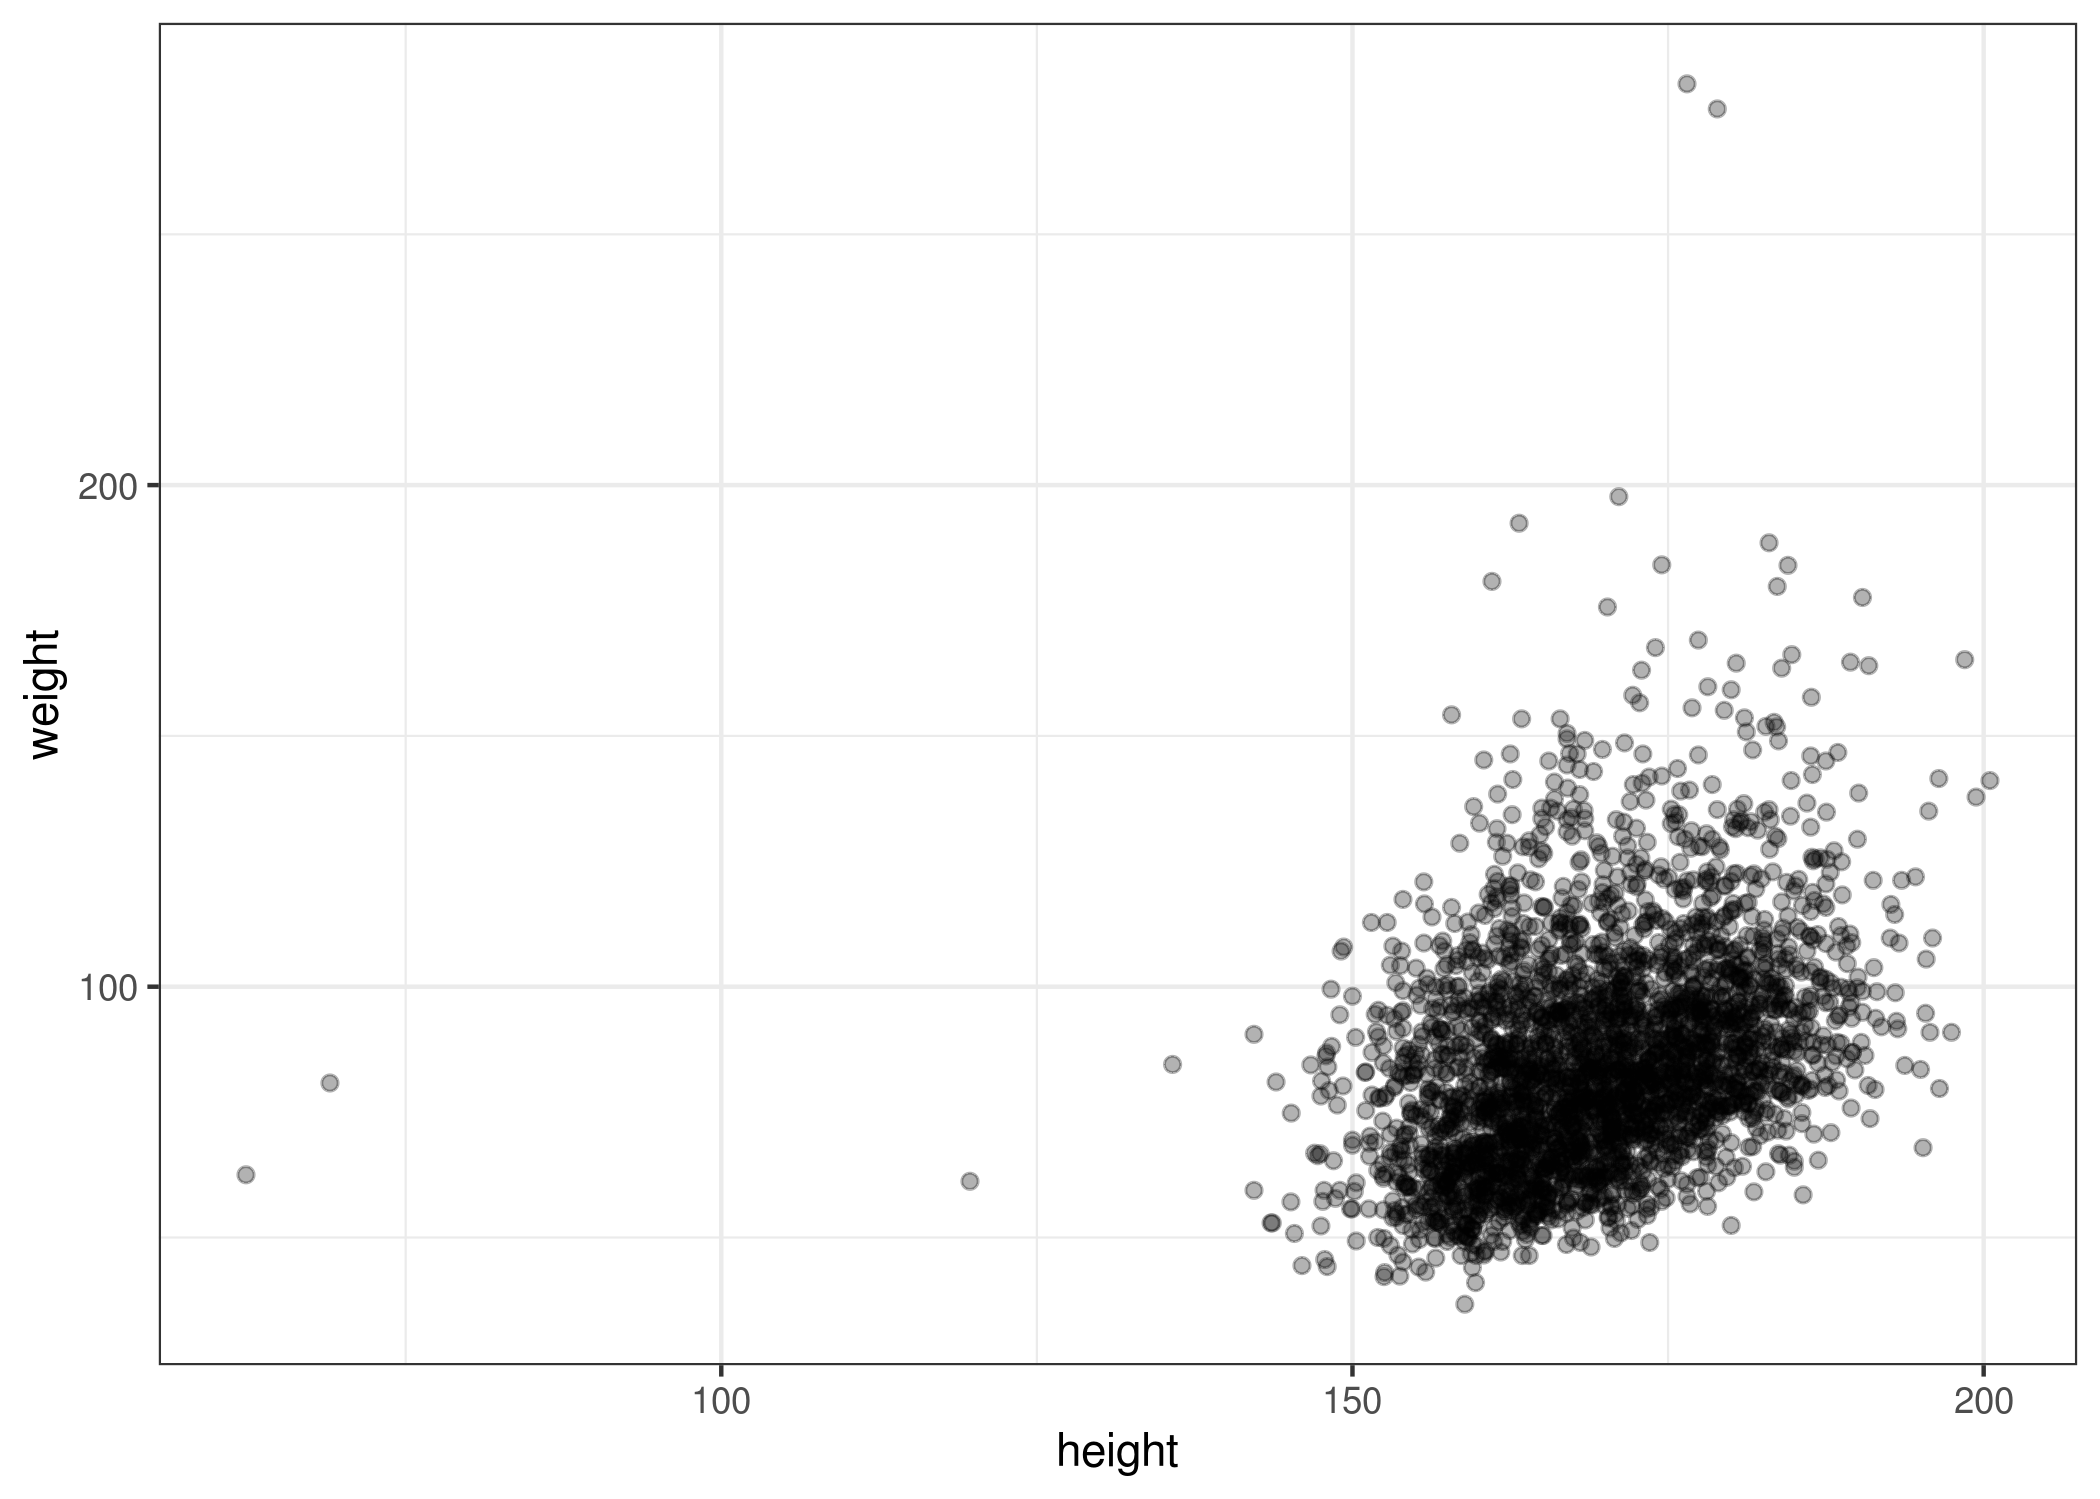
\includegraphics{figures/scatter_height_weight.png}

You can also utilize scatter plots when one of the variables is categorical. For example, we could be interested in the relationship between height and gender.

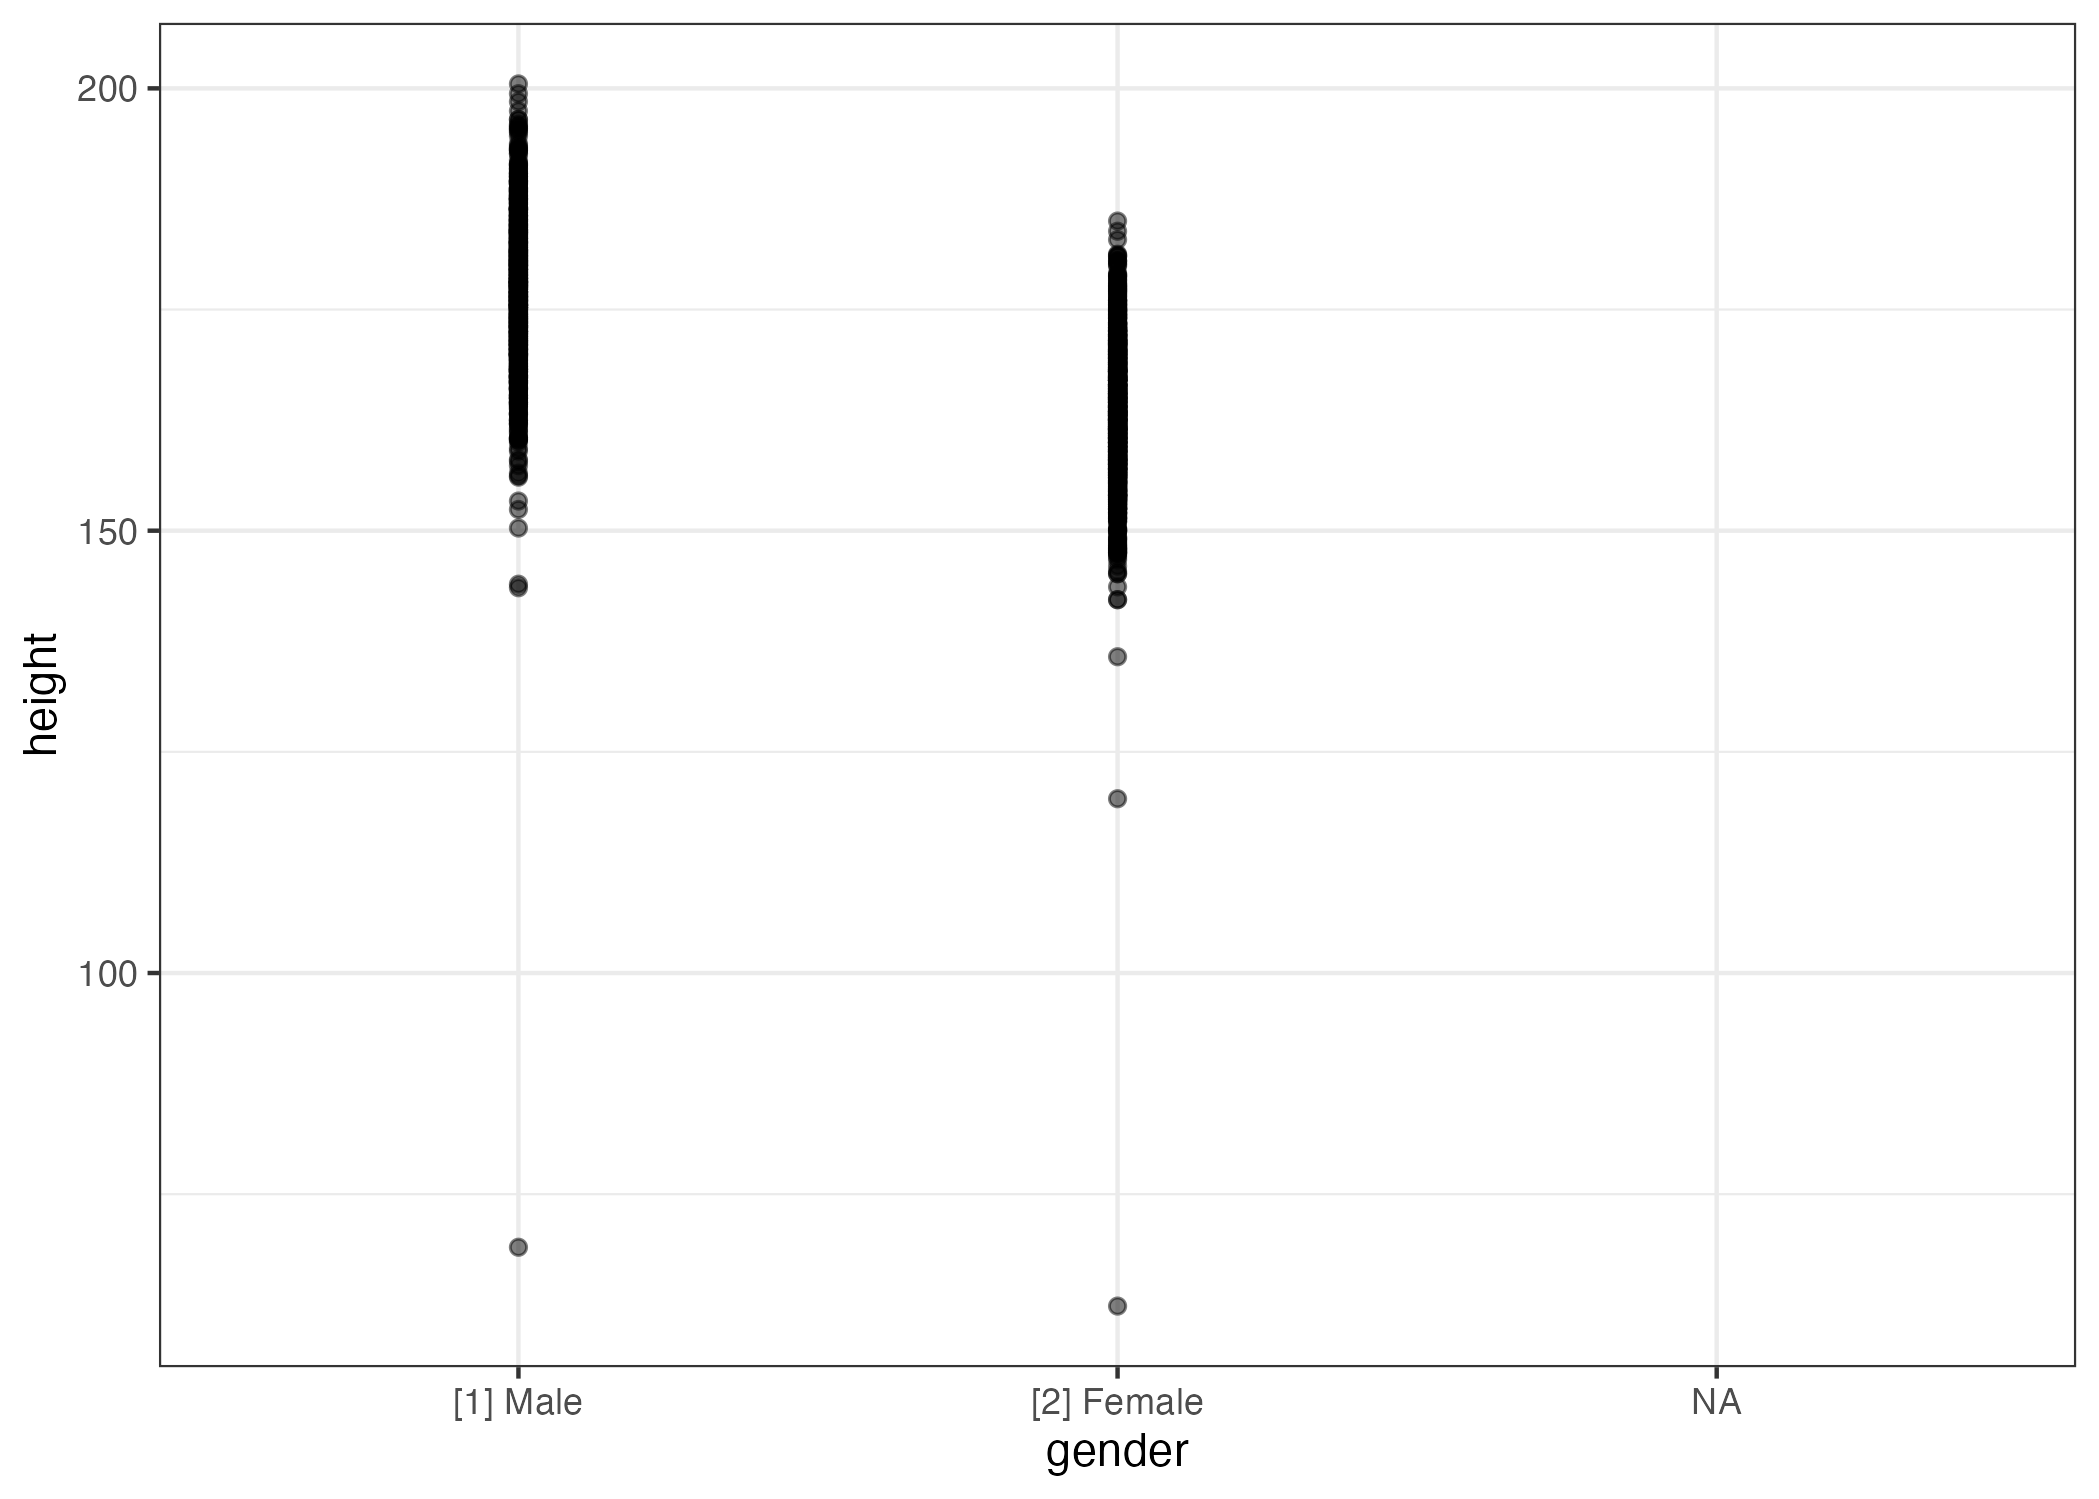
\includegraphics{figures/scatter_gender_height.png}

In this case, it can be beneficial to add a bit of jitter to the plot in the direction of the categorical variable.

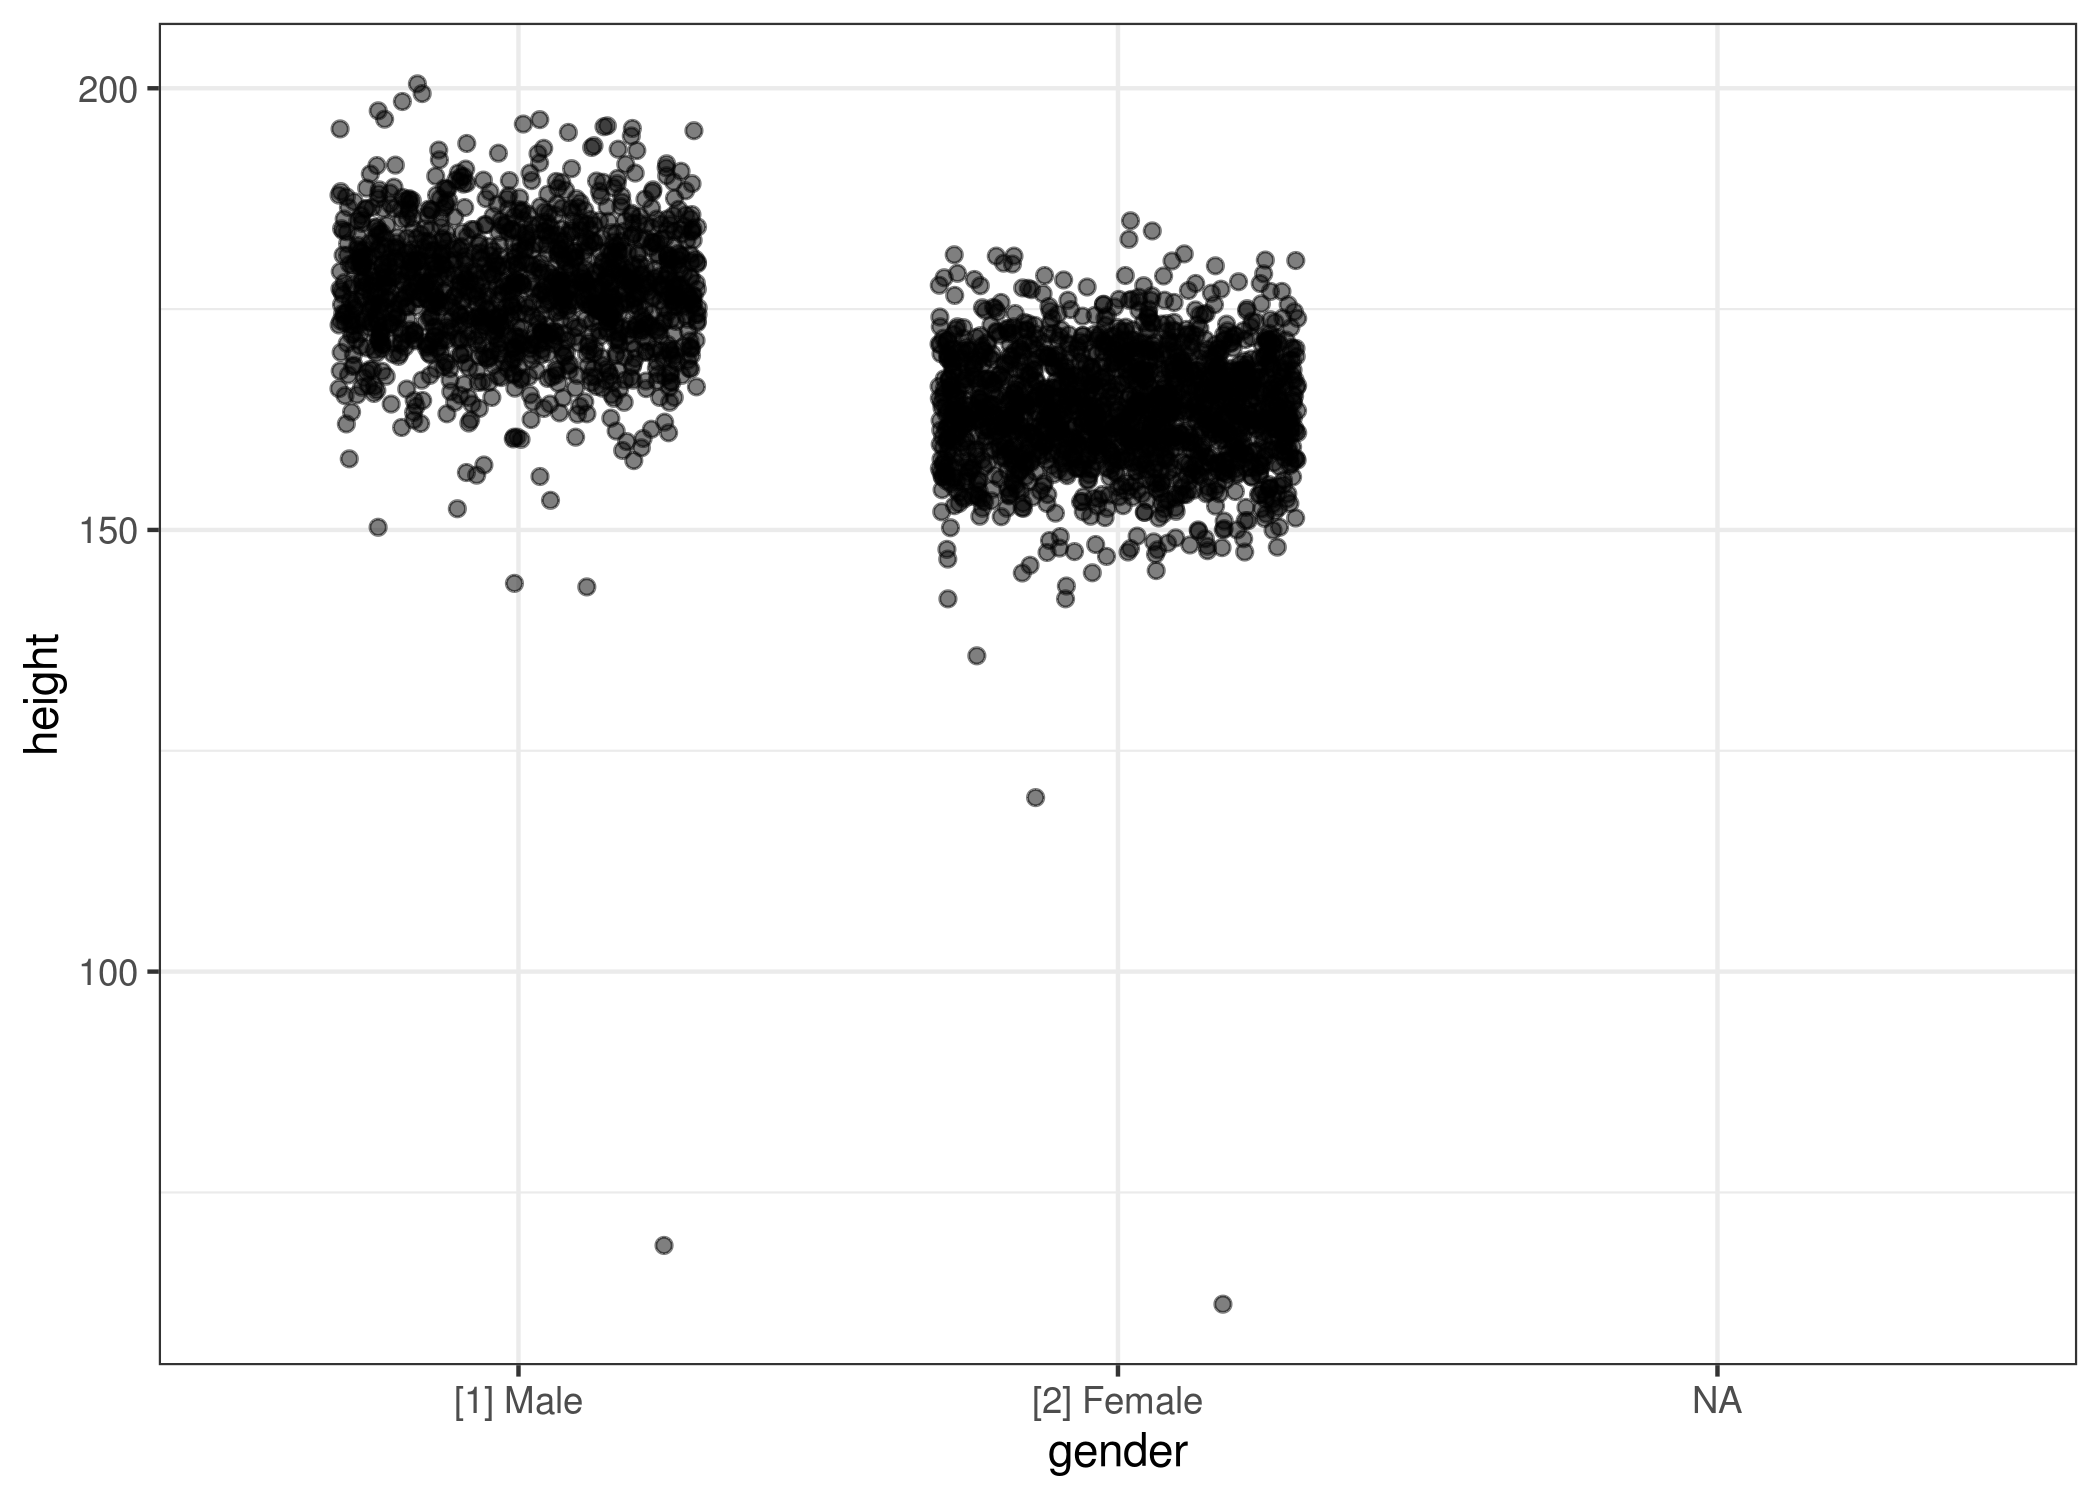
\includegraphics{figures/jitter_gender_height.png}

Even with a bit of jitter, it might be really hard to make anything of a scatter plot in this case, simply because we have ``too much'' data. In such a case, a boxplot might be a better choice.

\hypertarget{boxplots}{%
\subsection{Boxplots}\label{boxplots}}

Boxplots are great when you have a lot of data. They show the data through a set of summaries, namely the quartiles, and indicates if there are any \emph{outliers}. Below are boxplots for the height of the SHOW population by gender.

\includegraphics{figures/boxplot_gender_height.png}

You can use the figure below to decipher the box plot:

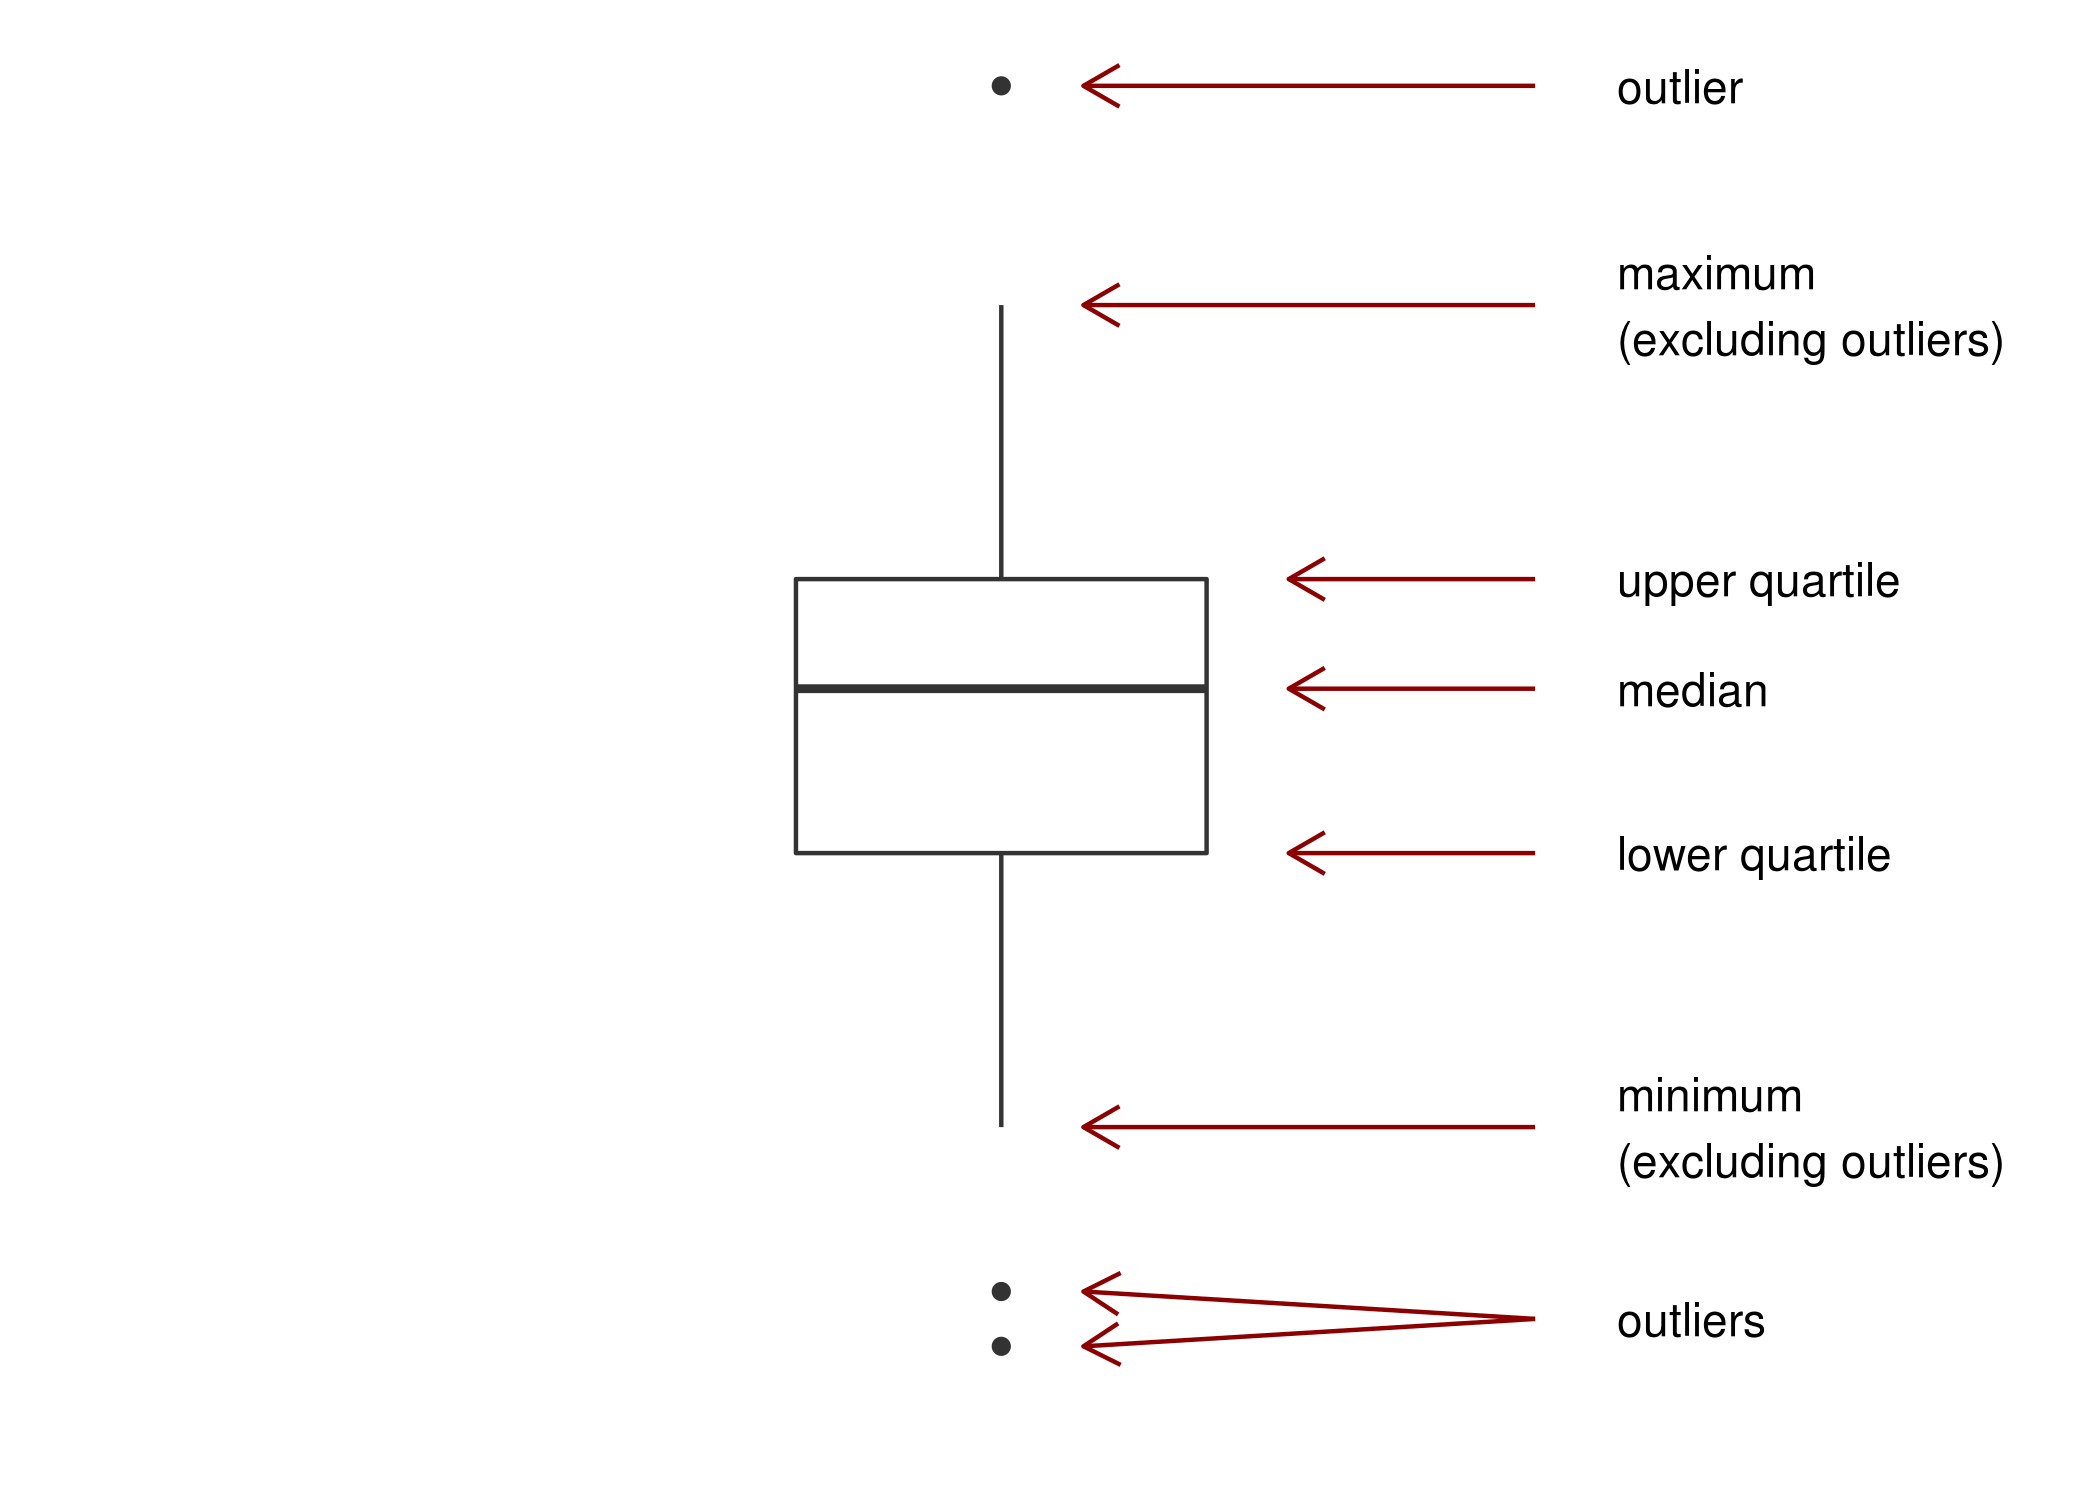
\includegraphics{figures/boxplot_explanation.png}

As you see on the boxplots of the SHOW data, it is a great tool to visualize continuous data when you have a lot of it. In a simple figure we can see that

\begin{itemize}
\tightlist
\item
  the median height is greater for men than women
\item
  there is generally a shift upwards for men compared to women
\item
  the 75\% tallest men are all taller than 75\% of women (compare the bottom of the box for men with the top of the box for women)
\end{itemize}

and much more.

One thing I haven't told you is the answer to a very important, very hard question: ``how do we decide if a data point is an outlier?'' We will simply adopt the practice that a data point is an outlier if it is more than 1.5 times the range of the box from the box. I.e. an observation is an outlier if it is greater than \(Q_3 + 1.5\cdot (Q_3 - Q_1)\) or less than \(Q_1 - 1.5\cdot (Q_3 - Q_1)\).

\hypertarget{histogram}{%
\subsection{Histogram}\label{histogram}}

At first, the \emph{histogram} looks a lot like a bar chart, but there are a few very important differences. Before we go into details, lets take a look at a histogram. Below is a histogram of the depression scores in the SHOW data set.

\includegraphics{figures/bmi_hist.png}

The main differences from a bar chart is that

\begin{enumerate}
\def\labelenumi{\arabic{enumi}.}
\tightlist
\item
  there are no gaps on the x-axis
\item
  the \emph{relative area} of a bar is the proportion of your sample that falls in the interval corresponding to that bar
\end{enumerate}

Later on, we will use the histogram to answer questions like ``what is the probability a randomly chosen individual from the SHOW population has a BMI greater than 40?'' or ``between 20 and 30?'' etc. This is simply done by dividing the area of the bars that are specified (for example all bars with BMI greater than 40) with the total area.

The histogram will be \textbf{super} important to us moving forward, so make sure you know how to decipher it!

\hypertarget{grey-areas}{%
\chapter{Grey areas}\label{grey-areas}}

An example of a variable that could easily be mistaken as categorical is age. Often when we think about age, we think about this in terms of years, or months, or even days. In that sense, age is a variable with a number of possible values that we could technically count -- start with 0, 1, 2, 3, \ldots, 55, 56, 57, \ldots{} . However, this is NOT the natural structure of the variable, but rather a limitation of the way it is measured and recorded. Technically, age is the time from birth till now, which if we could measure it with \emph{infinite} precision, could be any possible number\footnote{positive, real number, for those of you who want to be specific} you can think of.

Many other examples could be provided. In general, what's important to think about is the nature of the variable rather than what is measured. By nature, any measurement is going to be discrete, but some variables are continuous in nature.

\hypertarget{part-introduction-to-probability-random-variables}{%
\part{Introduction to Probability \& Random Variables}\label{part-introduction-to-probability-random-variables}}

Loosely based on \citet{ls} chapter 5.

\hypertarget{what-is-probability}{%
\chapter{What is ``probability''?}\label{what-is-probability}}

A \emph{probability} is a number between 0 and 1 that indicates how likely it is that a certain event happens. An event that has the probability of 1 \textbf{always} occurs, while an event with probability of 0 \textbf{never} occurs. Every number in between are a bit harder to interpret.

For example, an event with probability 0.5 supposedly happens every other time. This makes sense if you think about something that can be repeated, such as a coin flip, or the roll of a die, but how does that work if we consider an event that only occurs once? For example, how do we interpret a weather forecast that claims there's a 0.5 (i.e.~50\%) chance of rain tomorrow? We can only observe if it rains tomorrow once, so the probability surely must be 0 (it doesn't rain) or 1 (it rains), right?

\hypertarget{definitions}{%
\section{Definitions}\label{definitions}}

As hinted at above, the concept of ``probability'' can be a bit challenging to wrap your head around. There are generally two ways that the term is introduced. Though they are very similar once you understand the concepts, they can seem radically different at first.

\BeginKnitrBlock{definition}
\protect\hypertarget{def:prob-def-1}{}{\label{def:prob-def-1} }The probability of an event is the number of outcomes that ensure the event happens divided by the total number of possible outcomes, \textbf{IF} all outcomes are equally likely:

\[
  P(\text{event}) = \frac{\text{number of outcomes that result in event}}{\text{total number of possible outcomes}}.
\]
\EndKnitrBlock{definition}

We often refer to the numerator in this fraction as the number of favorable outcomes.

I want to take a second to draw your attention to that small, but incredibly important, final bit of the definition: ``IF all outcomes are equally likely''. We will later discuss what to do if this is not the case, but for now, this will be an underlying assumption.

The best way to become comfortable with this definition is by considering a few simple examples. The following two examples are the most commonly used, and (by far!!) most boring examples in the history of statistics. However, they are super useful for two reasons:

\begin{enumerate}
\def\labelenumi{\arabic{enumi}.}
\tightlist
\item
  They are so simple that it is possible to better grasp what's going on
\item
  A lot of more complicated examples can be simplified by comparing them to these two
\end{enumerate}

\hypertarget{examples-3}{%
\subsection{Examples}\label{examples-3}}

\hypertarget{coin-flip}{%
\subsubsection{Coin Flip}\label{coin-flip}}

We want to find the probability \(P(\text{coin comes up heads})\). A natural assumption is that when flipping a coin, heads and tails are the only outcomes\footnote{i.e.~it is NOT possible for the coin to land on the side}, and they are equally likely. Therefore,

\begin{align*}
  P(\text{coin comes up heads}) &= \frac{\text{number of possible outcomes that come up heads}}{\text{number of possible outcomes}} \\
  &= \frac{1}{2} \\
  &= 0.5.
\end{align*}

Similarly, one can find the probability that the coin comes up tails:

\begin{align}
  P(\text{coin comes up tails}) &= \frac{\text{number of possible outcomes that come up tails}}{\text{number of possible outcomes}} \\
  &= \frac{1}{2} \\
  &= 0.5.
\end{align}

\hypertarget{roll-of-a-die}{%
\subsubsection{Roll of a Die}\label{roll-of-a-die}}

Another classic example: calculate different probabilities when rolling a die. (Done in class -- see lecture notes.)

\begin{center}\rule{0.5\linewidth}{\linethickness}\end{center}

The two examples above show situations where all possible outcomes are equally likely. What if that is not the case?

\hypertarget{example-disease-status}{%
\subsection{Example: disease status}\label{example-disease-status}}

Let us consider the SHOW data set. We might be interested in the probability of a subject being obese. Now, there seems to be only two outcomes here: either the subject is obese, or the subject is not. So, using the same string of thoughts as above, one might conclude that the probability of a subject being obese if \(\frac{1}{2}\), i.e.~\(0.5\).

This is obviously not the case. The problem with this approach is that the two outcomes -- those being ``the subject is obese'', and ``the subject is NOT obese'' -- are not equally likely, so the simple approach of simply dividing the number of favorable outcomes by the number of possible outcomes is not doing us any good.

\begin{center}\rule{0.5\linewidth}{\linethickness}\end{center}

To find a more satisfying answer to the question asked in the last example, we need to consider a different approach to probabilities.

\BeginKnitrBlock{definition}
\protect\hypertarget{def:prob-def-2}{}{\label{def:prob-def-2} }The probability of a specific outcome from an experiment is the proportion of times the outcome occurs if the experiment is repeated an \emph{infinite number of times}.
\EndKnitrBlock{definition}

Repeating an experiment an infinite number of times is obviously not possible, so in practice ``an infinite number of times'' becomes ``a very large number of times''.

When introducing this different approach to probabilities, first we need to make sure it doesn't contradict our previous approach.

\hypertarget{example-coin-flip-revisited}{%
\subsection{Example: coin flip (revisited)}\label{example-coin-flip-revisited}}

We previously established that when flipping a coin, the probability of heads is \(0.5\). Hopefully this new definition will yield a similar answer.

To find out if that is actually the case, we would have to flip a coin ``an infinite number of times''. Obviously, this is not possible, so we will have to settle for ``a very large number of times''. So, imagine we flip a coin 100000 times. Every time it is flipped, we write down the result, and count how many times we've seen heads, and how many times we've seen tails so far. If the probability of seeing heads is \(0.5\), we should eventually see about as many heads as tails.

Below is an animation that shows the results of such an experiment. The bars show you the proportion of heads and tails, which in the end (by the definition above) will converge to the probability. The first 100 flips are all shown, then only the results after every 100 flips, and finally results after every 1000 flips are shown. Note how at the very end the two bars are both very close to \(0.5\).

\hypertarget{example-roll-of-a-die-revisited}{%
\subsection{Example: roll of a die (revisited)}\label{example-roll-of-a-die-revisited}}

Similarly to what we did above for the coin flip, we will do here for the roll of a die.

\hypertarget{example-disease-status-1}{%
\subsection{Example: disease status}\label{example-disease-status-1}}

Okay, so both when flipping a coin and rolling a die, the second definition agrees with the first one. But how can we use this way of thinking in the disease status example? What does it even mean to ``repeat the experiment'', let alone ``repeat an infinite number of times''?!

In such a situation, we make a (very crude, but very necessary) assumption: we assume that all the subjects in the cohort are ``similar enough'' that we can pretend that observing the disease status of multiple people constitutes multiple experiments. We then estimate the probability of having the disease as the proportion of subjects with the disease.

Let's consider the probability that a person from the SHOW population is mildly depressed. To estimate this, we simply divide the number of individuals in the population who are mildly depressed with the total number of people in the population.

Below are estimated probabilities for all depression severity levels. Note: \(P(\text{mildly depressed}) = \frac{454}{3381} \approx 0.134\).

\begin{longtable}[]{@{}ccc@{}}
\toprule
\begin{minipage}[b]{0.33\columnwidth}\centering
Depression Severity\strut
\end{minipage} & \begin{minipage}[b]{0.10\columnwidth}\centering
Count\strut
\end{minipage} & \begin{minipage}[b]{0.30\columnwidth}\centering
Estimated Probability\strut
\end{minipage}\tabularnewline
\midrule
\endhead
\begin{minipage}[t]{0.33\columnwidth}\centering
{[}1{]} No depression\strut
\end{minipage} & \begin{minipage}[t]{0.10\columnwidth}\centering
1629\strut
\end{minipage} & \begin{minipage}[t]{0.30\columnwidth}\centering
0.482\strut
\end{minipage}\tabularnewline
\begin{minipage}[t]{0.33\columnwidth}\centering
{[}2{]} Mild depression\strut
\end{minipage} & \begin{minipage}[t]{0.10\columnwidth}\centering
454\strut
\end{minipage} & \begin{minipage}[t]{0.30\columnwidth}\centering
0.134\strut
\end{minipage}\tabularnewline
\begin{minipage}[t]{0.33\columnwidth}\centering
{[}3{]} Moderate depression\strut
\end{minipage} & \begin{minipage}[t]{0.10\columnwidth}\centering
125\strut
\end{minipage} & \begin{minipage}[t]{0.30\columnwidth}\centering
0.037\strut
\end{minipage}\tabularnewline
\begin{minipage}[t]{0.33\columnwidth}\centering
{[}4{]} Moderately severe
depression\strut
\end{minipage} & \begin{minipage}[t]{0.10\columnwidth}\centering
52\strut
\end{minipage} & \begin{minipage}[t]{0.30\columnwidth}\centering
0.0154\strut
\end{minipage}\tabularnewline
\begin{minipage}[t]{0.33\columnwidth}\centering
{[}5{]} Severe depression\strut
\end{minipage} & \begin{minipage}[t]{0.10\columnwidth}\centering
15\strut
\end{minipage} & \begin{minipage}[t]{0.30\columnwidth}\centering
0.00444\strut
\end{minipage}\tabularnewline
\begin{minipage}[t]{0.33\columnwidth}\centering
NA\strut
\end{minipage} & \begin{minipage}[t]{0.10\columnwidth}\centering
1106\strut
\end{minipage} & \begin{minipage}[t]{0.30\columnwidth}\centering
0.327\strut
\end{minipage}\tabularnewline
\begin{minipage}[t]{0.33\columnwidth}\centering
Total\strut
\end{minipage} & \begin{minipage}[t]{0.10\columnwidth}\centering
3381\strut
\end{minipage} & \begin{minipage}[t]{0.30\columnwidth}\centering
1\strut
\end{minipage}\tabularnewline
\bottomrule
\end{longtable}

\hypertarget{conditional-probability}{%
\chapter{Conditional Probability}\label{conditional-probability}}

So far, we have talked about probabilities in a context where no additional information is available about the experiment. This is of course not always the case, and also not always what we are interested in.

A useful concept in these cases is the concept of \emph{conditional probabilities}. In a nutshell, conditional probabilities deal with the chances of something happening given something else has already happened. If we consider two events, \(A\) and \(B\), then we write \(P(A | B)\) for the conditional probability of \(A\) given that \(B\) has happened, and read it as ``the (conditional) probability of \(A\) given \(B\)''.

\hypertarget{example-roll-a-die}{%
\section{Example: roll a die}\label{example-roll-a-die}}

Previously, we considered the probabilities associated with the roll of a die. We found that the probability of rolling a six is \(\frac{1}{6}\). What if we somehow knew that the outcome turned out to be an even number, but simply didn't know which even number? Well, using this information, we know there are only three possible outcomes, namely \(2,4,6\). They are all equally likely, so using definition \ref{def:prob-def-1}, we find that the probability of rolling a six given the roll comes up even is

\[\left .P(\text{roll a } 6\ \right|\ \text{roll is even}) = \frac{1}{3}.\]

\hypertarget{example-disease-status-2}{%
\section{Example: disease status}\label{example-disease-status-2}}

In the last section we found \(P(\text{mild depression}) \approx 0.134\). Let us try to calculate the conditional probability of having a mild depression \emph{given} the subject is divorced. The way to do this is to first create the two way contingency table:

\begin{longtable}[]{@{}cccccccccc@{}}
\toprule
\begin{minipage}[b]{0.12\columnwidth}\centering
Depression Severity\strut
\end{minipage} & \begin{minipage}[b]{0.08\columnwidth}\centering
{[}.D{]} Don't know\strut
\end{minipage} & \begin{minipage}[b]{0.06\columnwidth}\centering
{[}1{]} Married\strut
\end{minipage} & \begin{minipage}[b]{0.06\columnwidth}\centering
{[}2{]} Widowed\strut
\end{minipage} & \begin{minipage}[b]{0.07\columnwidth}\centering
{[}3{]} Divorced\strut
\end{minipage} & \begin{minipage}[b]{0.07\columnwidth}\centering
{[}4{]} Separated\strut
\end{minipage} & \begin{minipage}[b]{0.09\columnwidth}\centering
{[}5{]} Never married\strut
\end{minipage} & \begin{minipage}[b]{0.12\columnwidth}\centering
{[}6{]} Living with partner\strut
\end{minipage} & \begin{minipage}[b]{0.03\columnwidth}\centering
NA\_\strut
\end{minipage} & \begin{minipage}[b]{0.04\columnwidth}\centering
Total\strut
\end{minipage}\tabularnewline
\midrule
\endhead
\begin{minipage}[t]{0.12\columnwidth}\centering
{[}1{]} No depression\strut
\end{minipage} & \begin{minipage}[t]{0.08\columnwidth}\centering
1\strut
\end{minipage} & \begin{minipage}[t]{0.06\columnwidth}\centering
1102\strut
\end{minipage} & \begin{minipage}[t]{0.06\columnwidth}\centering
57\strut
\end{minipage} & \begin{minipage}[t]{0.07\columnwidth}\centering
174\strut
\end{minipage} & \begin{minipage}[t]{0.07\columnwidth}\centering
12\strut
\end{minipage} & \begin{minipage}[t]{0.09\columnwidth}\centering
239\strut
\end{minipage} & \begin{minipage}[t]{0.12\columnwidth}\centering
43\strut
\end{minipage} & \begin{minipage}[t]{0.03\columnwidth}\centering
1\strut
\end{minipage} & \begin{minipage}[t]{0.04\columnwidth}\centering
1629\strut
\end{minipage}\tabularnewline
\begin{minipage}[t]{0.12\columnwidth}\centering
{[}2{]} Mild depression\strut
\end{minipage} & \begin{minipage}[t]{0.08\columnwidth}\centering
0\strut
\end{minipage} & \begin{minipage}[t]{0.06\columnwidth}\centering
253\strut
\end{minipage} & \begin{minipage}[t]{0.06\columnwidth}\centering
17\strut
\end{minipage} & \begin{minipage}[t]{0.07\columnwidth}\centering
76\strut
\end{minipage} & \begin{minipage}[t]{0.07\columnwidth}\centering
4\strut
\end{minipage} & \begin{minipage}[t]{0.09\columnwidth}\centering
84\strut
\end{minipage} & \begin{minipage}[t]{0.12\columnwidth}\centering
19\strut
\end{minipage} & \begin{minipage}[t]{0.03\columnwidth}\centering
1\strut
\end{minipage} & \begin{minipage}[t]{0.04\columnwidth}\centering
454\strut
\end{minipage}\tabularnewline
\begin{minipage}[t]{0.12\columnwidth}\centering
{[}3{]} Moderate depression\strut
\end{minipage} & \begin{minipage}[t]{0.08\columnwidth}\centering
0\strut
\end{minipage} & \begin{minipage}[t]{0.06\columnwidth}\centering
55\strut
\end{minipage} & \begin{minipage}[t]{0.06\columnwidth}\centering
1\strut
\end{minipage} & \begin{minipage}[t]{0.07\columnwidth}\centering
27\strut
\end{minipage} & \begin{minipage}[t]{0.07\columnwidth}\centering
3\strut
\end{minipage} & \begin{minipage}[t]{0.09\columnwidth}\centering
33\strut
\end{minipage} & \begin{minipage}[t]{0.12\columnwidth}\centering
6\strut
\end{minipage} & \begin{minipage}[t]{0.03\columnwidth}\centering
0\strut
\end{minipage} & \begin{minipage}[t]{0.04\columnwidth}\centering
125\strut
\end{minipage}\tabularnewline
\begin{minipage}[t]{0.12\columnwidth}\centering
{[}4{]} Moderately severe
depression\strut
\end{minipage} & \begin{minipage}[t]{0.08\columnwidth}\centering
0\strut
\end{minipage} & \begin{minipage}[t]{0.06\columnwidth}\centering
13\strut
\end{minipage} & \begin{minipage}[t]{0.06\columnwidth}\centering
4\strut
\end{minipage} & \begin{minipage}[t]{0.07\columnwidth}\centering
15\strut
\end{minipage} & \begin{minipage}[t]{0.07\columnwidth}\centering
1\strut
\end{minipage} & \begin{minipage}[t]{0.09\columnwidth}\centering
13\strut
\end{minipage} & \begin{minipage}[t]{0.12\columnwidth}\centering
6\strut
\end{minipage} & \begin{minipage}[t]{0.03\columnwidth}\centering
0\strut
\end{minipage} & \begin{minipage}[t]{0.04\columnwidth}\centering
52\strut
\end{minipage}\tabularnewline
\begin{minipage}[t]{0.12\columnwidth}\centering
{[}5{]} Severe depression\strut
\end{minipage} & \begin{minipage}[t]{0.08\columnwidth}\centering
0\strut
\end{minipage} & \begin{minipage}[t]{0.06\columnwidth}\centering
7\strut
\end{minipage} & \begin{minipage}[t]{0.06\columnwidth}\centering
1\strut
\end{minipage} & \begin{minipage}[t]{0.07\columnwidth}\centering
3\strut
\end{minipage} & \begin{minipage}[t]{0.07\columnwidth}\centering
1\strut
\end{minipage} & \begin{minipage}[t]{0.09\columnwidth}\centering
2\strut
\end{minipage} & \begin{minipage}[t]{0.12\columnwidth}\centering
1\strut
\end{minipage} & \begin{minipage}[t]{0.03\columnwidth}\centering
0\strut
\end{minipage} & \begin{minipage}[t]{0.04\columnwidth}\centering
15\strut
\end{minipage}\tabularnewline
\begin{minipage}[t]{0.12\columnwidth}\centering
NA\strut
\end{minipage} & \begin{minipage}[t]{0.08\columnwidth}\centering
1\strut
\end{minipage} & \begin{minipage}[t]{0.06\columnwidth}\centering
645\strut
\end{minipage} & \begin{minipage}[t]{0.06\columnwidth}\centering
33\strut
\end{minipage} & \begin{minipage}[t]{0.07\columnwidth}\centering
121\strut
\end{minipage} & \begin{minipage}[t]{0.07\columnwidth}\centering
20\strut
\end{minipage} & \begin{minipage}[t]{0.09\columnwidth}\centering
232\strut
\end{minipage} & \begin{minipage}[t]{0.12\columnwidth}\centering
51\strut
\end{minipage} & \begin{minipage}[t]{0.03\columnwidth}\centering
3\strut
\end{minipage} & \begin{minipage}[t]{0.04\columnwidth}\centering
1106\strut
\end{minipage}\tabularnewline
\begin{minipage}[t]{0.12\columnwidth}\centering
Total\strut
\end{minipage} & \begin{minipage}[t]{0.08\columnwidth}\centering
2\strut
\end{minipage} & \begin{minipage}[t]{0.06\columnwidth}\centering
2075\strut
\end{minipage} & \begin{minipage}[t]{0.06\columnwidth}\centering
113\strut
\end{minipage} & \begin{minipage}[t]{0.07\columnwidth}\centering
416\strut
\end{minipage} & \begin{minipage}[t]{0.07\columnwidth}\centering
41\strut
\end{minipage} & \begin{minipage}[t]{0.09\columnwidth}\centering
603\strut
\end{minipage} & \begin{minipage}[t]{0.12\columnwidth}\centering
126\strut
\end{minipage} & \begin{minipage}[t]{0.03\columnwidth}\centering
5\strut
\end{minipage} & \begin{minipage}[t]{0.04\columnwidth}\centering
3381\strut
\end{minipage}\tabularnewline
\bottomrule
\end{longtable}

To find the conditional probability, you basically narrow down the universe you operate in. Instead of asking ``how many individuals have mild depression out of all individuals?'' you ask ``how many individuals have mild depression out of \textbf{individuals that are divorced}?''. So, in other words, all you worry about is the column in the table corresponding to the divorced subjects. We estimate the conditional probability of having a mild depression given the subject is divorced as \(P(\text{mild depression} | \text{divorced}) = \frac{76}{416} \approx 0.183\).

\begin{longtable}[]{@{}cccccccccc@{}}
\toprule
\begin{minipage}[b]{0.12\columnwidth}\centering
Depression Severity\strut
\end{minipage} & \begin{minipage}[b]{0.08\columnwidth}\centering
{[}.D{]} Don't know\strut
\end{minipage} & \begin{minipage}[b]{0.06\columnwidth}\centering
{[}1{]} Married\strut
\end{minipage} & \begin{minipage}[b]{0.06\columnwidth}\centering
{[}2{]} Widowed\strut
\end{minipage} & \begin{minipage}[b]{0.07\columnwidth}\centering
{[}3{]} Divorced\strut
\end{minipage} & \begin{minipage}[b]{0.07\columnwidth}\centering
{[}4{]} Separated\strut
\end{minipage} & \begin{minipage}[b]{0.09\columnwidth}\centering
{[}5{]} Never married\strut
\end{minipage} & \begin{minipage}[b]{0.12\columnwidth}\centering
{[}6{]} Living with partner\strut
\end{minipage} & \begin{minipage}[b]{0.03\columnwidth}\centering
NA\_\strut
\end{minipage} & \begin{minipage}[b]{0.04\columnwidth}\centering
Total\strut
\end{minipage}\tabularnewline
\midrule
\endhead
\begin{minipage}[t]{0.12\columnwidth}\centering
{[}1{]} No depression\strut
\end{minipage} & \begin{minipage}[t]{0.08\columnwidth}\centering
1\strut
\end{minipage} & \begin{minipage}[t]{0.06\columnwidth}\centering
1102\strut
\end{minipage} & \begin{minipage}[t]{0.06\columnwidth}\centering
57\strut
\end{minipage} & \begin{minipage}[t]{0.07\columnwidth}\centering
\textbf{174}\strut
\end{minipage} & \begin{minipage}[t]{0.07\columnwidth}\centering
12\strut
\end{minipage} & \begin{minipage}[t]{0.09\columnwidth}\centering
239\strut
\end{minipage} & \begin{minipage}[t]{0.12\columnwidth}\centering
43\strut
\end{minipage} & \begin{minipage}[t]{0.03\columnwidth}\centering
1\strut
\end{minipage} & \begin{minipage}[t]{0.04\columnwidth}\centering
1629\strut
\end{minipage}\tabularnewline
\begin{minipage}[t]{0.12\columnwidth}\centering
{[}2{]} Mild depression\strut
\end{minipage} & \begin{minipage}[t]{0.08\columnwidth}\centering
0\strut
\end{minipage} & \begin{minipage}[t]{0.06\columnwidth}\centering
253\strut
\end{minipage} & \begin{minipage}[t]{0.06\columnwidth}\centering
17\strut
\end{minipage} & \begin{minipage}[t]{0.07\columnwidth}\centering
\textbf{76}\strut
\end{minipage} & \begin{minipage}[t]{0.07\columnwidth}\centering
4\strut
\end{minipage} & \begin{minipage}[t]{0.09\columnwidth}\centering
84\strut
\end{minipage} & \begin{minipage}[t]{0.12\columnwidth}\centering
19\strut
\end{minipage} & \begin{minipage}[t]{0.03\columnwidth}\centering
1\strut
\end{minipage} & \begin{minipage}[t]{0.04\columnwidth}\centering
454\strut
\end{minipage}\tabularnewline
\begin{minipage}[t]{0.12\columnwidth}\centering
{[}3{]} Moderate depression\strut
\end{minipage} & \begin{minipage}[t]{0.08\columnwidth}\centering
0\strut
\end{minipage} & \begin{minipage}[t]{0.06\columnwidth}\centering
55\strut
\end{minipage} & \begin{minipage}[t]{0.06\columnwidth}\centering
1\strut
\end{minipage} & \begin{minipage}[t]{0.07\columnwidth}\centering
\textbf{27}\strut
\end{minipage} & \begin{minipage}[t]{0.07\columnwidth}\centering
3\strut
\end{minipage} & \begin{minipage}[t]{0.09\columnwidth}\centering
33\strut
\end{minipage} & \begin{minipage}[t]{0.12\columnwidth}\centering
6\strut
\end{minipage} & \begin{minipage}[t]{0.03\columnwidth}\centering
0\strut
\end{minipage} & \begin{minipage}[t]{0.04\columnwidth}\centering
125\strut
\end{minipage}\tabularnewline
\begin{minipage}[t]{0.12\columnwidth}\centering
{[}4{]} Moderately severe
depression\strut
\end{minipage} & \begin{minipage}[t]{0.08\columnwidth}\centering
0\strut
\end{minipage} & \begin{minipage}[t]{0.06\columnwidth}\centering
13\strut
\end{minipage} & \begin{minipage}[t]{0.06\columnwidth}\centering
4\strut
\end{minipage} & \begin{minipage}[t]{0.07\columnwidth}\centering
\textbf{15}\strut
\end{minipage} & \begin{minipage}[t]{0.07\columnwidth}\centering
1\strut
\end{minipage} & \begin{minipage}[t]{0.09\columnwidth}\centering
13\strut
\end{minipage} & \begin{minipage}[t]{0.12\columnwidth}\centering
6\strut
\end{minipage} & \begin{minipage}[t]{0.03\columnwidth}\centering
0\strut
\end{minipage} & \begin{minipage}[t]{0.04\columnwidth}\centering
52\strut
\end{minipage}\tabularnewline
\begin{minipage}[t]{0.12\columnwidth}\centering
{[}5{]} Severe depression\strut
\end{minipage} & \begin{minipage}[t]{0.08\columnwidth}\centering
0\strut
\end{minipage} & \begin{minipage}[t]{0.06\columnwidth}\centering
7\strut
\end{minipage} & \begin{minipage}[t]{0.06\columnwidth}\centering
1\strut
\end{minipage} & \begin{minipage}[t]{0.07\columnwidth}\centering
\textbf{3}\strut
\end{minipage} & \begin{minipage}[t]{0.07\columnwidth}\centering
1\strut
\end{minipage} & \begin{minipage}[t]{0.09\columnwidth}\centering
2\strut
\end{minipage} & \begin{minipage}[t]{0.12\columnwidth}\centering
1\strut
\end{minipage} & \begin{minipage}[t]{0.03\columnwidth}\centering
0\strut
\end{minipage} & \begin{minipage}[t]{0.04\columnwidth}\centering
15\strut
\end{minipage}\tabularnewline
\begin{minipage}[t]{0.12\columnwidth}\centering
NA\strut
\end{minipage} & \begin{minipage}[t]{0.08\columnwidth}\centering
1\strut
\end{minipage} & \begin{minipage}[t]{0.06\columnwidth}\centering
645\strut
\end{minipage} & \begin{minipage}[t]{0.06\columnwidth}\centering
33\strut
\end{minipage} & \begin{minipage}[t]{0.07\columnwidth}\centering
\textbf{121}\strut
\end{minipage} & \begin{minipage}[t]{0.07\columnwidth}\centering
20\strut
\end{minipage} & \begin{minipage}[t]{0.09\columnwidth}\centering
232\strut
\end{minipage} & \begin{minipage}[t]{0.12\columnwidth}\centering
51\strut
\end{minipage} & \begin{minipage}[t]{0.03\columnwidth}\centering
3\strut
\end{minipage} & \begin{minipage}[t]{0.04\columnwidth}\centering
1106\strut
\end{minipage}\tabularnewline
\begin{minipage}[t]{0.12\columnwidth}\centering
Total\strut
\end{minipage} & \begin{minipage}[t]{0.08\columnwidth}\centering
2\strut
\end{minipage} & \begin{minipage}[t]{0.06\columnwidth}\centering
2075\strut
\end{minipage} & \begin{minipage}[t]{0.06\columnwidth}\centering
113\strut
\end{minipage} & \begin{minipage}[t]{0.07\columnwidth}\centering
\textbf{416}\strut
\end{minipage} & \begin{minipage}[t]{0.07\columnwidth}\centering
41\strut
\end{minipage} & \begin{minipage}[t]{0.09\columnwidth}\centering
603\strut
\end{minipage} & \begin{minipage}[t]{0.12\columnwidth}\centering
126\strut
\end{minipage} & \begin{minipage}[t]{0.03\columnwidth}\centering
5\strut
\end{minipage} & \begin{minipage}[t]{0.04\columnwidth}\centering
3381\strut
\end{minipage}\tabularnewline
\bottomrule
\end{longtable}

\hypertarget{example-sensitivityspecificity}{%
\section{Example: Sensitivity/specificity}\label{example-sensitivityspecificity}}

Two important examples of conditional probabilities are the so-called sensitivity and specificity. These are particularly useful when discussing the accuracy of screening tests.

The \emph{sensitivity} of a test is the \emph{true positive rate} (or fraction). That is, out of the tests performed on individuals with the disease of interest, how many come out positive. I.e. \(\text{sensitivity} = P(\text{test positive}\ |\ \text{individual diseased})\).

Similarly, the \emph{specificity} of a test is the \emph{true negative rate} (or fraction), i.e.~the proportion of tests performed on healthy individuals that come out negative: \(\text{specificity} = P(\text{test negative}\ |\ \text{individual healthy})\).

It is also often useful to consider the \emph{false positive rate} (FPR) and \emph{false negative rate} (FNR). These are defined as follows:

\begin{align*}
  \text{FPR} &= P(\text{test positive}\ |\ \text{individual healthy}), \\
  \text{FNR} &= P(\text{test negative}\ |\ \text{individual diseased}). \\
\end{align*}

Let's consider a concrete example. Below is table 5-5 from \citet{ls}. This table shows the results of screenings of 4810 pregnant women to assess if their fetus is likely to have Down Syndrome. After birth, it is determined if the child actually has Down Syndrome, provided a ground truth that we can check our screening method against. Ideally, the test is positive for all kids with Down Syndrome, and negative for alld kids without Down Syndrome.

\hypertarget{htmlwidget-c618f2bd1060fb3dd51e}{}

Let us calculate the specificity, sensitivity, FNR, and FPR:

\begin{align*}
  \text{specificity} &= P(\text{test negative}\ |\ \text{child healthy}) \\
                     &= \frac{\text{number of negative tests among healthy children}}{\text{number of healthy children}} \\
                     &= \frac{4449}{4800} = 0.927 \\
                     & \\
  \text{sensitivity} &= P(\text{test positive}\ |\ \text{child has Down Syndrome}) \\
                     &= \frac{\text{number of positive tests among children with Down Syndrome}}{\text{number of children with Down Syndrome}} \\
                     &= \frac{9}{10} = 0.9 \\
                     & \\
  \text{FPR} &= P(\text{test positive}\ |\ \text{individual healthy}) \\
             &= \frac{\text{number of positive tests among healthy children}}{\text{number of healthy children}} \\
             &= \frac{351}{4800} = 0.073 \\
             & \\
  \text{FNR} &= P(\text{test negative}\ |\ \text{individual diseased}) \\
             &= \frac{\text{number of negative tests among children with Down Syndrome}}{\text{number of children with Down Syndrome}} \\
             &= \frac{1}{10} = 0.1.
\end{align*}

We see that the test has some very desirable attributes, in high specificity AND high sensitivity. At this point, some might stop and wonder for a second: the end goal is to determine if the test is accurate, so why don't we just calculate the accuracy of the test? I.e. what's wrong at simply looking at the number of corret test results out of the total number of tests? Let's take a look.

\begin{align*}
  \text{test accuracy} &= \frac{\text{number of correct results}}{\text{number of tests performed}} \\
                       &= \frac{9 + 4449}{4810} \\
                       &= \frac{4458}{4810} = 0.927
\end{align*}

That's pretty impressive. The test has an accuracy rate of almost \(93\%\), i.e.~almost \(93\%\) of tests yield the correct result. Now, let us consider a different test for the same disease. Tested on the same 4810 women, and pretend it yields the following results:

\hypertarget{htmlwidget-17ea6fb7bd90fbb45135}{}

Now, the accuracy rate of this test is \(\frac{1 + 4449}{4810} = 0.925\), i.e.~almost the same as the first test. That's, again, really impressive! But upon further investigation, something is off. The sensitivity is way off. Out of 10 children with Down Syndrome, the test only came back positive for 1, which yields a sensitivity of only only \(0.1\). In other words, if a fetus actually is a affected, the test only has a \(10\%\) chance of detecting it. That's not very comforting.

This is a common problem with rare diseases. Since by far most individuals will not be diseased, a test that is good at predicting healthy individuals, but awful at predicting diseased individuals, will have a high accuracy, but such a test is not very desirable. Consider this last test for Down Syndrome: no test is performed, and we just always say the fetus is unaffected. Since 4800 out of 4810 fetuses were unaffected, we have an accuracy of \(\frac{4800}{4810} = 0.998\). Pretty impressive accuracy rate, absolutely useless test\ldots{}

\hypertarget{example-positivenegative-predictive-value}{%
\section{Example: positive/negative predictive value}\label{example-positivenegative-predictive-value}}

The specificity is the answer to the question ``what is the probability the test will be correct when the patient is actually healthy?'' This is of course a very important thing to know, and if this probability is very low, the test might not be particularly useful. However, a just as important, and sometimes more relevant, measure is the \emph{negative predictive value}. This relates to the question ``what is the probability the patient is actually healthy when the test comes back negative?''

Similarly, we can talk about the \emph{positive predictive value}. Where the sensitivity is the probability that the test is positive if the patient has the disease, the positive predictive value is the probability that a patient has the disease if the test comes back positive.

Let us again consider the Down Syndrome data. Since the positive predictive value is the probability a child has Down Syndrome given the test is positive, it is calculated as the proportion of children with positive tests that actually had the disease. So,

\begin{align*}
  \text{Positive Predictive Value} &= P(\text{child diseased } | \text{ test positive}) \\
                                   &= \frac{9}{360} \\
                                   &= 0.025.
\end{align*}

Similarly, the negative predictive value is the probability a child is healthy given the test was negative. This is calculated as the proportion of children with negative tests that actually are healthy. So,

\begin{align*}
  \text{Negative Predictive Value} &= P(\text{child healthy } | \text{ test negative}) \\
                                   &= \frac{4449}{4450} \\
                                   &= 0.999.
\end{align*}

\hypertarget{bayes-theorem}{%
\section{Bayes' Theorem}\label{bayes-theorem}}

We have seen a few examples of some very useful and meaningful quantities that are actually conditional probabilities. We've seen how we, in general, calculate these conditional probabilities, but only in a setting where we know everything. The following theorem\footnote{to those who are not familiar with the math jargon: theorem = very big and important result} provides a powerful way of finding conditional probabilities, and it also provides a very useful connection between conditional probabilities, and marginal probabilities (i.e.~probabilities that are not conditional).

\BeginKnitrBlock{theorem}[Bayes' Theorem]
\protect\hypertarget{thm:bayes}{}{\label{thm:bayes} \iffalse (Bayes' Theorem) \fi{} }Bayes' Theorem simply states that

\[
P(A | B) = \frac{P(A \text{ and } B)}{P(B)} \label{eq:bayes1},
\]

or equivalently

\[
P(A | B) = \frac{P(B | A)P(A)}{P(B)} \label{eq:bayes2}
\]
\EndKnitrBlock{theorem}

Since \(P(A \text{ and } B) = P(B \text{ and } A)\), equation \eqref{eq:bayes1} gives us that \(P(B | A)P(A) = P(A \text{ and } B)\), and so equation \eqref{eq:bayes2} follows by plugging this into the numerator in equation \eqref{eq:bayes1}.

Especially the latter formulation is very powerful, as we shall see in this next example.

\hypertarget{example-5.8-in-ls-positive-predictive-value-from-sensitivity}{%
\subsection{\texorpdfstring{Example (5.8 in \citet{ls}): positive predictive value from sensitivity}{Example (5.8 in @ls): positive predictive value from sensitivity}}\label{example-5.8-in-ls-positive-predictive-value-from-sensitivity}}

Bayes' Theorem allows us to calculate the positive predictive value using the sensitivity of a test, the prevalence of the disease we're testing for, and how often the test itself is positive (regardless of patient status).

Consider a situation where a disease is really rare with a prevalence of \(0.2\%\) (i.e.~\(2\) in \(1000\) individuals have the disease). A screening test for this disease has a reported sensitivity of \(85\%\), comes back positive \(8\%\) of the time, and negative \(92\%\) of the time.

We would like to know what the positive predictive value is, i.e.~\(P(\text{patient has the disease} | \text{screen positive})\). Using Bayes' rule, we know

\begin{align*}
  &P(\text{patient has the disease} | \text{screen positive}) = \\
  &\hspace{2cm} \frac{P(\text{screen positive} | \text{patient has the disease}) \cdot P(\text{patient has the disease})}{P(\text{screen positive})}
\end{align*}

Notice: \(P(\text{screen positive} | \text{patient has the disease})\) is exactly the sensitivity, \(P(\text{patient has the disease})\) is the prevalence, and \(P(\text{screen positive})\) is the probability the screening test comes back positive. We know all these probabilities, and so we can calculate the positive predictive value.

\begin{align*}
  \text{PPV} &= P(\text{patient has the disease} | \text{screen positive}) \\
             &= \frac{P(\text{screen positive} | \text{patient has the disease}) \cdot P(\text{patient has the disease})}{P(\text{screen positive})} \\
             &= \frac{0.85 \cdot 0.002}{0.08} \approx 0.021
\end{align*}

\hypertarget{independence}{%
\section{Independence}\label{independence}}

One of the big concepts in statistics in general is the concept of independence. When things are independent, all the math simplifies a great deal, which is the main reason why a lot of the methods we will consider later on are based on the assumption that observations are independent of one another.

Loosely speaking, two events are said to be \emph{independent} if knowledge about one of the events does not provide any information about the other. I.e. if I ask you what the probabilitity of event A before and after I tell you whether event B happened or not, your answers should be the same.

\hypertarget{example-independent-events}{%
\subsection{Example: independent events}\label{example-independent-events}}

Event A: I walk around Madison one day, stop a random stranger, and ask: ``are you taller than 6ft?''

Event B: I flip a coin, and it comes up tails.

Events A and B are independent. The probability that a random person is taller than 6ft is not altered by the fact that a coin flip comes up tails.

\hypertarget{example-dependent-events}{%
\subsection{Example: dependent events}\label{example-dependent-events}}

Event A: I walk around Madison one day, stop a random stranger, and ask: ``are you taller than 6ft?''

Event B: The random stranger I stop is male.

Events A and B are NOT independent. The probability a random stranger is taller than 6ft is about 0.16 if the person is male, but less than 0.01 if the person is female.\footnote{loosely based on data from \url{https://dqydj.com/height-percentile-calculator-for-men-and-women/}} So the probability of event A being `yes' depends on the outcome of event B. Therefore, they are not independent.

\begin{center}\rule{0.5\linewidth}{\linethickness}\end{center}

We will work with two definitions of independence. (Fortunately, they are equivalent, i.e.~if one holds, the other holds.)

\BeginKnitrBlock{definition}
\protect\hypertarget{def:ind1}{}{\label{def:ind1} }Two events are independent if and only if \(P(A \text{ and } B) = P(A) P(B)\).
\EndKnitrBlock{definition}

\BeginKnitrBlock{definition}
\protect\hypertarget{def:ind2}{}{\label{def:ind2} }Two events are independent if and only if \(P(A | B) = P(A)\) \textbf{AND} \(P(B | A) = P(B)\).
\EndKnitrBlock{definition}

\hypertarget{example-are-depression-severity-mild-depression-and-marital-status-divorced-independent}{%
\subsection{Example: are ``depression severity = mild depression'' and ``marital status = divorced'' independent?}\label{example-are-depression-severity-mild-depression-and-marital-status-divorced-independent}}

Let's say that \(A = \text{subject is divorced}\) and \(B = \text{subject is mildly depressed}\). For simplicity, we only consider subjects for which we know both marital status and depression severity, i.e.~any subjects with missing data in one of the two variables have been removed.

The contingency table:

\begin{longtable}[]{@{}cccc@{}}
\toprule
\begin{minipage}[b]{0.27\columnwidth}\centering
Depression Severity\strut
\end{minipage} & \begin{minipage}[b]{0.14\columnwidth}\centering
Divorced\strut
\end{minipage} & \begin{minipage}[b]{0.18\columnwidth}\centering
Not divorced\strut
\end{minipage} & \begin{minipage}[b]{0.10\columnwidth}\centering
Total\strut
\end{minipage}\tabularnewline
\midrule
\endhead
\begin{minipage}[t]{0.27\columnwidth}\centering
mild depression\strut
\end{minipage} & \begin{minipage}[t]{0.14\columnwidth}\centering
76\strut
\end{minipage} & \begin{minipage}[t]{0.18\columnwidth}\centering
377\strut
\end{minipage} & \begin{minipage}[t]{0.10\columnwidth}\centering
453\strut
\end{minipage}\tabularnewline
\begin{minipage}[t]{0.27\columnwidth}\centering
not mild depression\strut
\end{minipage} & \begin{minipage}[t]{0.14\columnwidth}\centering
219\strut
\end{minipage} & \begin{minipage}[t]{0.18\columnwidth}\centering
1601\strut
\end{minipage} & \begin{minipage}[t]{0.10\columnwidth}\centering
1820\strut
\end{minipage}\tabularnewline
\begin{minipage}[t]{0.27\columnwidth}\centering
Total\strut
\end{minipage} & \begin{minipage}[t]{0.14\columnwidth}\centering
295\strut
\end{minipage} & \begin{minipage}[t]{0.18\columnwidth}\centering
1978\strut
\end{minipage} & \begin{minipage}[t]{0.10\columnwidth}\centering
2273\strut
\end{minipage}\tabularnewline
\bottomrule
\end{longtable}

Now, we can test for independence in two different ways: either using definition \ref{def:ind1} or definition \ref{def:ind2}. Let's do both.

Using definition \ref{def:ind1}, we need to calculate three probabilities:

\begin{align*}
  P(A \text{ and } B) &= P(\text{divorced and mildly depressed}) = \frac{76}{2273} \approx 0.0334 \\
  & \\
  P(A) &= P(\text{divorced}) = \frac{295}{2273} \approx 0.1298 \\
  & \\
  P(B) &= P(\text{mild depression}) = \frac{453}{2273} \approx 0.1993
\end{align*}

Since \(P(A)\cdot P(B) \approx 0.1298 \cdot 0.1993 \approx 0.0258691\), which is NOT the same as \(P(A \text{ and } B) = 0.0334\), these two events are not independent of each other.

Using definition \ref{def:ind2}, we need to calculate four probabilities. Two of them, \(P(A)\) and \(P(B)\), we already calculated. Let's calculate the remaining two:

\begin{align*}
  P(A | B) &= P(\text{divorced} | \text{mildly depressed}) = \frac{76}{453} \approx 0.1678\\
  & \\
  P(B | A) &= P(\text{mildly depressed} | \text{divorced}) = \frac{76}{295} \approx 0.2576
\end{align*}

As you can see, \(P(A | B) \neq P(A)\) and \(P(B | A) \neq P(B)\), so again, the conclusion is that the two events are not independent of one another.

What if we instead let \(A = \text{subject is male}\) and \(B = \text{subject is married}\)? The contingency table:

\begin{longtable}[]{@{}ccccccccc@{}}
\toprule
\begin{minipage}[b]{0.07\columnwidth}\centering
gender\strut
\end{minipage} & \begin{minipage}[b]{0.10\columnwidth}\centering
{[}.D{]} Don't know\strut
\end{minipage} & \begin{minipage}[b]{0.07\columnwidth}\centering
{[}1{]} Married\strut
\end{minipage} & \begin{minipage}[b]{0.07\columnwidth}\centering
{[}2{]} Widowed\strut
\end{minipage} & \begin{minipage}[b]{0.08\columnwidth}\centering
{[}3{]} Divorced\strut
\end{minipage} & \begin{minipage}[b]{0.08\columnwidth}\centering
{[}4{]} Separated\strut
\end{minipage} & \begin{minipage}[b]{0.11\columnwidth}\centering
{[}5{]} Never married\strut
\end{minipage} & \begin{minipage}[b]{0.14\columnwidth}\centering
{[}6{]} Living with partner\strut
\end{minipage} & \begin{minipage}[b]{0.04\columnwidth}\centering
Total\strut
\end{minipage}\tabularnewline
\midrule
\endhead
\begin{minipage}[t]{0.07\columnwidth}\centering
{[}1{]} Male\strut
\end{minipage} & \begin{minipage}[t]{0.10\columnwidth}\centering
1\strut
\end{minipage} & \begin{minipage}[t]{0.07\columnwidth}\centering
928\strut
\end{minipage} & \begin{minipage}[t]{0.07\columnwidth}\centering
31\strut
\end{minipage} & \begin{minipage}[t]{0.08\columnwidth}\centering
153\strut
\end{minipage} & \begin{minipage}[t]{0.08\columnwidth}\centering
8\strut
\end{minipage} & \begin{minipage}[t]{0.11\columnwidth}\centering
303\strut
\end{minipage} & \begin{minipage}[t]{0.14\columnwidth}\centering
53\strut
\end{minipage} & \begin{minipage}[t]{0.04\columnwidth}\centering
1477\strut
\end{minipage}\tabularnewline
\begin{minipage}[t]{0.07\columnwidth}\centering
{[}2{]} Female\strut
\end{minipage} & \begin{minipage}[t]{0.10\columnwidth}\centering
1\strut
\end{minipage} & \begin{minipage}[t]{0.07\columnwidth}\centering
1147\strut
\end{minipage} & \begin{minipage}[t]{0.07\columnwidth}\centering
82\strut
\end{minipage} & \begin{minipage}[t]{0.08\columnwidth}\centering
263\strut
\end{minipage} & \begin{minipage}[t]{0.08\columnwidth}\centering
33\strut
\end{minipage} & \begin{minipage}[t]{0.11\columnwidth}\centering
300\strut
\end{minipage} & \begin{minipage}[t]{0.14\columnwidth}\centering
73\strut
\end{minipage} & \begin{minipage}[t]{0.04\columnwidth}\centering
1899\strut
\end{minipage}\tabularnewline
\begin{minipage}[t]{0.07\columnwidth}\centering
Total\strut
\end{minipage} & \begin{minipage}[t]{0.10\columnwidth}\centering
2\strut
\end{minipage} & \begin{minipage}[t]{0.07\columnwidth}\centering
2075\strut
\end{minipage} & \begin{minipage}[t]{0.07\columnwidth}\centering
113\strut
\end{minipage} & \begin{minipage}[t]{0.08\columnwidth}\centering
416\strut
\end{minipage} & \begin{minipage}[t]{0.08\columnwidth}\centering
41\strut
\end{minipage} & \begin{minipage}[t]{0.11\columnwidth}\centering
603\strut
\end{minipage} & \begin{minipage}[t]{0.14\columnwidth}\centering
126\strut
\end{minipage} & \begin{minipage}[t]{0.04\columnwidth}\centering
3376\strut
\end{minipage}\tabularnewline
\bottomrule
\end{longtable}

Let us just check using definition \ref{def:ind1}:

\begin{align*}
  P(A \text{ and } B) &= P(\text{male and married}) = \frac{928}{3376} \approx 0.2749 \\
  & \\
  P(A) &= P(\text{male}) = \frac{1477}{3376} \approx 0.4375 \\
  & \\
  P(B) &= P(\text{married}) = \frac{2075}{3376} \approx 0.6146
\end{align*}

So \(P(A)\cdot P(B) \approx 0.2689\), which is not very different from \(P(A \text{ and } B)\). Seems reasonable to say that these events indeed are independent.

\begin{center}\rule{0.5\linewidth}{\linethickness}\end{center}

While definition \ref{def:ind1} is very useful when doing math, it might not make a whole lot of sense intuitively. Definition \ref{def:ind2}, on the other hand, aligns with our intuitive understanding of independence.

Intuitively, two events, \(A\) and \(B\), are independent if \(A\) provides no information about \(B\), and vice versa. Now, if \(A\) provides no information about \(B\), then what would the difference between \(P(B)\) and \(P(B|A)\) be? Remember, the latter is basically the probability of \(B\) if \(A\) happens. But if \(A\) and \(B\) are independent, \(A\) provides no information about \(B\), so the probability of \(B\) doesn't change if \(A\) happens.

\hypertarget{random-variables-and-distributions}{%
\chapter{Random Variables and Distributions}\label{random-variables-and-distributions}}

So far in this section, we've talked about probabilities, different ways of thinking about probabilities, and a bit about how to work with probabilities. In this section we will introduce a more formal framework for how to think about and handle uncertain events. By making a few assumptions about how things behave, we can calculate probabilities of events without observing them.

\hypertarget{random-variables}{%
\section{Random Variables}\label{random-variables}}

A \emph{random variable} is a variable where the value is not guarenteed in advance, but can take different values.

\hypertarget{examples-random-variables}{%
\subsection{Examples: random variables}\label{examples-random-variables}}

Define a variable \(X\) to be the outcome of a coin flip. Now, before we flip the coin, we do not know what value \(X\) will take on -- it could be ``heads'' or it could be ``tails''. Once we flip the coin and observe the outcome, we say that we have a \emph{realization} of the random variable \(X\).

Another example would be if we let \(Y\) be the height of a randomly chosen US adult. We don't know exactly what value it is, but we do know a few things about it. For example, it is much more likely to be around 5.5ft than it is to be around 7ft or below 4ft. When we do finally randomly select a US adult, and measure their height, we get a realization of this random variable.

A third example is if we let \(Z\) denote the diabetes status of a randomly chosen US adult. This could take the values healthy, type I, or type II, and each will happen with some probability.

\hypertarget{distributions}{%
\section{Distributions}\label{distributions}}

As the example above was meant to illustrate, a random variable can really be anything you'd like. Whenever we talk about a random variable, we also talk about the probability of certain outcomes. If we can define a way to calculate probabilities of different outcomes of the random variable, we call this the \emph{distribution} of the random variable.

Recall previously we talked about two kinds of variables: \protect\hyperlink{discrete}{discrete} and \protect\hyperlink{continuous}{continuous} variables. Likewise, we can consider both discrete and continuous \emph{random} variables. Depending on the kind of random variable we're discussing, defining it's distribution is handled slightly differently.

The distribution of a random variable is super important for one reason: if you know the distribution, you know everything! The distribution allows you to calculate any probability you could ever be interested in, and therefore a lot of what follows has to do with specifying the distributions of different random variables.

\hypertarget{discrete-distributions}{%
\subsection{Discrete Distributions}\label{discrete-distributions}}

When we consider discrete random variables, its distribution is defined by specifying the probability of every single possible outcome. There are two things that are important to remember:

\begin{enumerate}
\def\labelenumi{\arabic{enumi}.}
\tightlist
\item
  all probabilities must be between \(0\) and \(1\),
\item
  the sum of all probabilities must add up to \(1\).
\end{enumerate}

The second point above is important, and is sometimes super handy when trying to calculate probabilities of certain complicated events. The intuition behind it is pretty simple: something must happen. So the probability that something happens is \(1\).

\hypertarget{examples-4}{%
\subsubsection{Examples:}\label{examples-4}}

Let \(X\) be a disrete random variables that can attain the values \(1,2,3,4,5\).

One possible distribution \(X\) could follow is given in the table below:

\begin{longtable}[]{@{}cc@{}}
\toprule
\begin{minipage}[b]{0.05\columnwidth}\centering
x\strut
\end{minipage} & \begin{minipage}[b]{0.14\columnwidth}\centering
P(X = x)\strut
\end{minipage}\tabularnewline
\midrule
\endhead
\begin{minipage}[t]{0.05\columnwidth}\centering
1\strut
\end{minipage} & \begin{minipage}[t]{0.14\columnwidth}\centering
0.2\strut
\end{minipage}\tabularnewline
\begin{minipage}[t]{0.05\columnwidth}\centering
2\strut
\end{minipage} & \begin{minipage}[t]{0.14\columnwidth}\centering
0.5\strut
\end{minipage}\tabularnewline
\begin{minipage}[t]{0.05\columnwidth}\centering
3\strut
\end{minipage} & \begin{minipage}[t]{0.14\columnwidth}\centering
0.1\strut
\end{minipage}\tabularnewline
\begin{minipage}[t]{0.05\columnwidth}\centering
4\strut
\end{minipage} & \begin{minipage}[t]{0.14\columnwidth}\centering
0.05\strut
\end{minipage}\tabularnewline
\begin{minipage}[t]{0.05\columnwidth}\centering
5\strut
\end{minipage} & \begin{minipage}[t]{0.14\columnwidth}\centering
0.15\strut
\end{minipage}\tabularnewline
\bottomrule
\end{longtable}

Another possible distribution is

\begin{longtable}[]{@{}cc@{}}
\toprule
\begin{minipage}[b]{0.05\columnwidth}\centering
x\strut
\end{minipage} & \begin{minipage}[b]{0.14\columnwidth}\centering
P(X = x)\strut
\end{minipage}\tabularnewline
\midrule
\endhead
\begin{minipage}[t]{0.05\columnwidth}\centering
1\strut
\end{minipage} & \begin{minipage}[t]{0.14\columnwidth}\centering
0.9\strut
\end{minipage}\tabularnewline
\begin{minipage}[t]{0.05\columnwidth}\centering
2\strut
\end{minipage} & \begin{minipage}[t]{0.14\columnwidth}\centering
0.025\strut
\end{minipage}\tabularnewline
\begin{minipage}[t]{0.05\columnwidth}\centering
3\strut
\end{minipage} & \begin{minipage}[t]{0.14\columnwidth}\centering
0.025\strut
\end{minipage}\tabularnewline
\begin{minipage}[t]{0.05\columnwidth}\centering
4\strut
\end{minipage} & \begin{minipage}[t]{0.14\columnwidth}\centering
0.025\strut
\end{minipage}\tabularnewline
\begin{minipage}[t]{0.05\columnwidth}\centering
5\strut
\end{minipage} & \begin{minipage}[t]{0.14\columnwidth}\centering
0.025\strut
\end{minipage}\tabularnewline
\bottomrule
\end{longtable}

Note that in both cases 1) we have specified the probabilities of all possible outcomes, 2) all probabilities are between \(0\) and \(1\), and 3) the probabilities add up to \(1\).

Using the latter distribution, we can calculate all sorts of probabilities:

\begin{align*}
  P(X = 3 \text{ or } X = 4) &= 0.025 + 0.025 = 0.05 \\
  & \\
  P(X < 3) &= 0.9 + 0.025 = 0.925 \\
  & \\
  P(3 < X < 5) &= 0.025 \\
  & \\
  P(X = 2 \text{ and } X = 5) &= 0
\end{align*}

\hypertarget{continuous-distributions}{%
\subsection{Continuous distributions}\label{continuous-distributions}}

The distribution of a continuous variable is specified by a curve that covers all possible values of the variable. Where for a discrete distribution the sum of all probabilities must add up to \(1\), for a continuous distribution the area under the curve must be \(1\).

Recall that the distribution of a random variable allows us to calculate probabilities of any possible events related to the random variable.

There are two questions we need to answer:

\begin{enumerate}
\def\labelenumi{\arabic{enumi}.}
\tightlist
\item
  How do we figure out what the curve looks like if we don't know the distributions?
\item
  How do we use the curve to calculate probabilities?
\end{enumerate}

Let's start with the first question.

Remember how we interpret probabilities per definition \ref{def:prob-def-2} (``the long run proportion of times an event happens''), and how we noticed how proportions could be found using a \protect\hyperlink{histogram}{histogram} (as the area of bars corresponding to the event divided by the total area). To find the distribution of a random variable, we would (if we could\ldots) in some sense combine the two: observe the outcome of the random variable many, many, many times, then create a histogram with very narrow bars.

The animation below illustrates this. Here we pretend that we observe the outcome of a random variable \(X\) many, many times. We continuously draw a histogram of the values we've seen so far.

Notice how as we get more observations, we make the bars more and more narrow. In the end, it is not hard to imagine a curve where we once had bars. This ``curve'' is what is formally known as the \emph{density} of the distribution of the random variable \(X\). Below is the histogram of all \(1,000,000\) observations shown with an exponential distribution with rate parameter 2 overlaid. This is actually the distribution I used to create the outcomes of \(X\). This justifies this way of thining about the creation of a distribution.

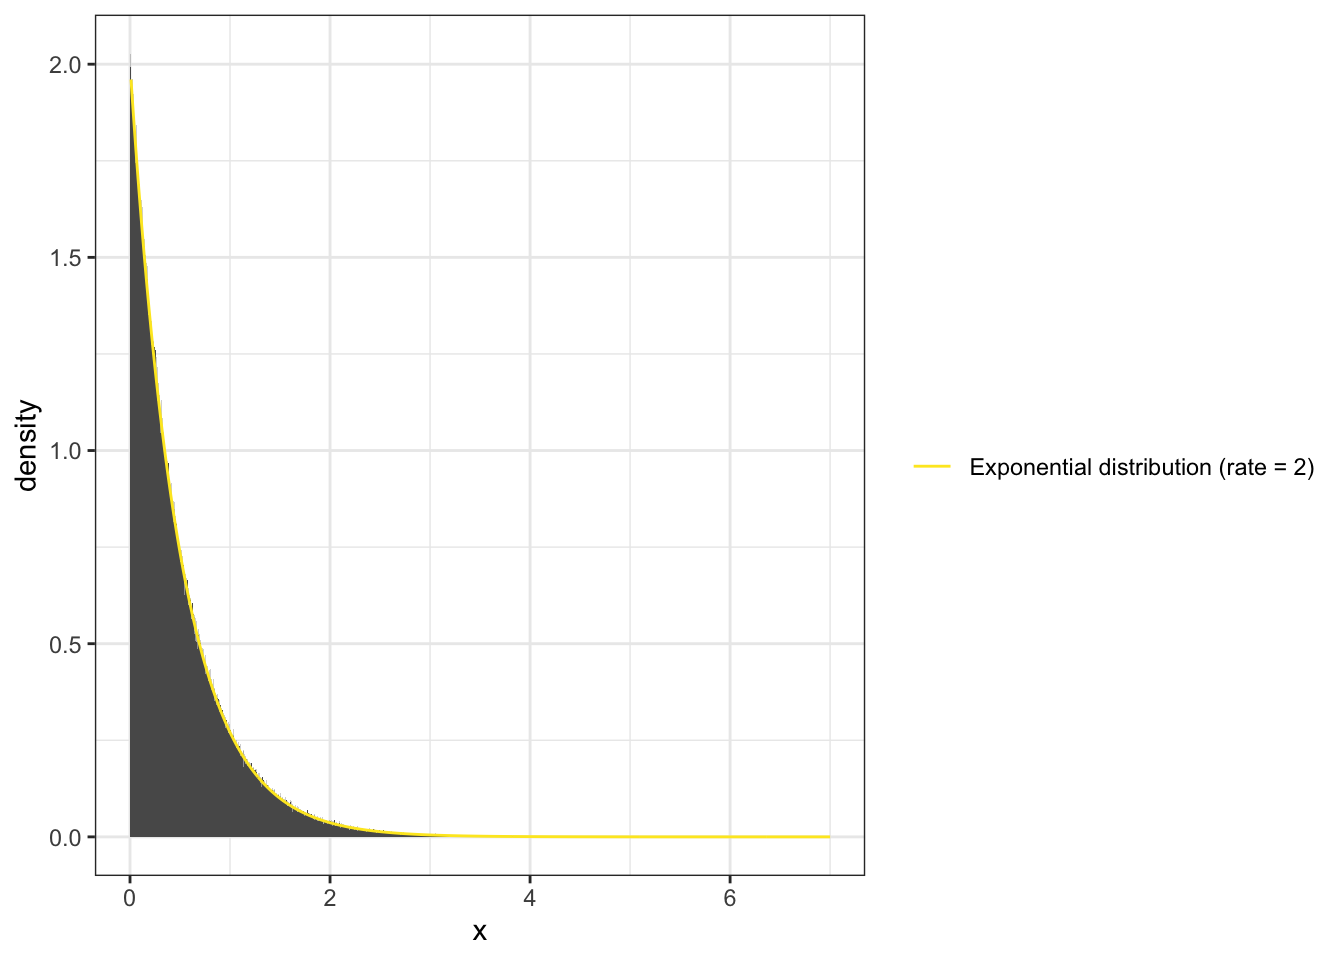
\includegraphics{783_biostats_files/figure-latex/unnamed-chunk-28-1.pdf}

We have now seen how we can, at least theoretically, find the distribution of a random variable. You can imagine doing the same thing with real data, except we cannot observe the outcome as many times as we'd like. Below is the distribution of the height of participants in the show data.

\hypertarget{htmlwidget-4ba537f5e22a1317c3f2}{}

As we go along, the line between the ``distribution'' of a random variable, and the ``histogram'' of the observations will probably be blurred. That's okay. As we just saw, the histogram turns into the distribution with enough observations. In many ways, the histogram is our best guess to the distribution of a random variable (unless we're willing to make some assumption, as we'll see later). This is exactly why I like the histogram to display continuous data -- when you know the distribution, you know everything, and the histogram is the closest we can get to the distribution!

So how do we use this information to calculate probabilities? Areas under the curve. Let's pretend the height of SHOW participants follows the distribution depicted below:

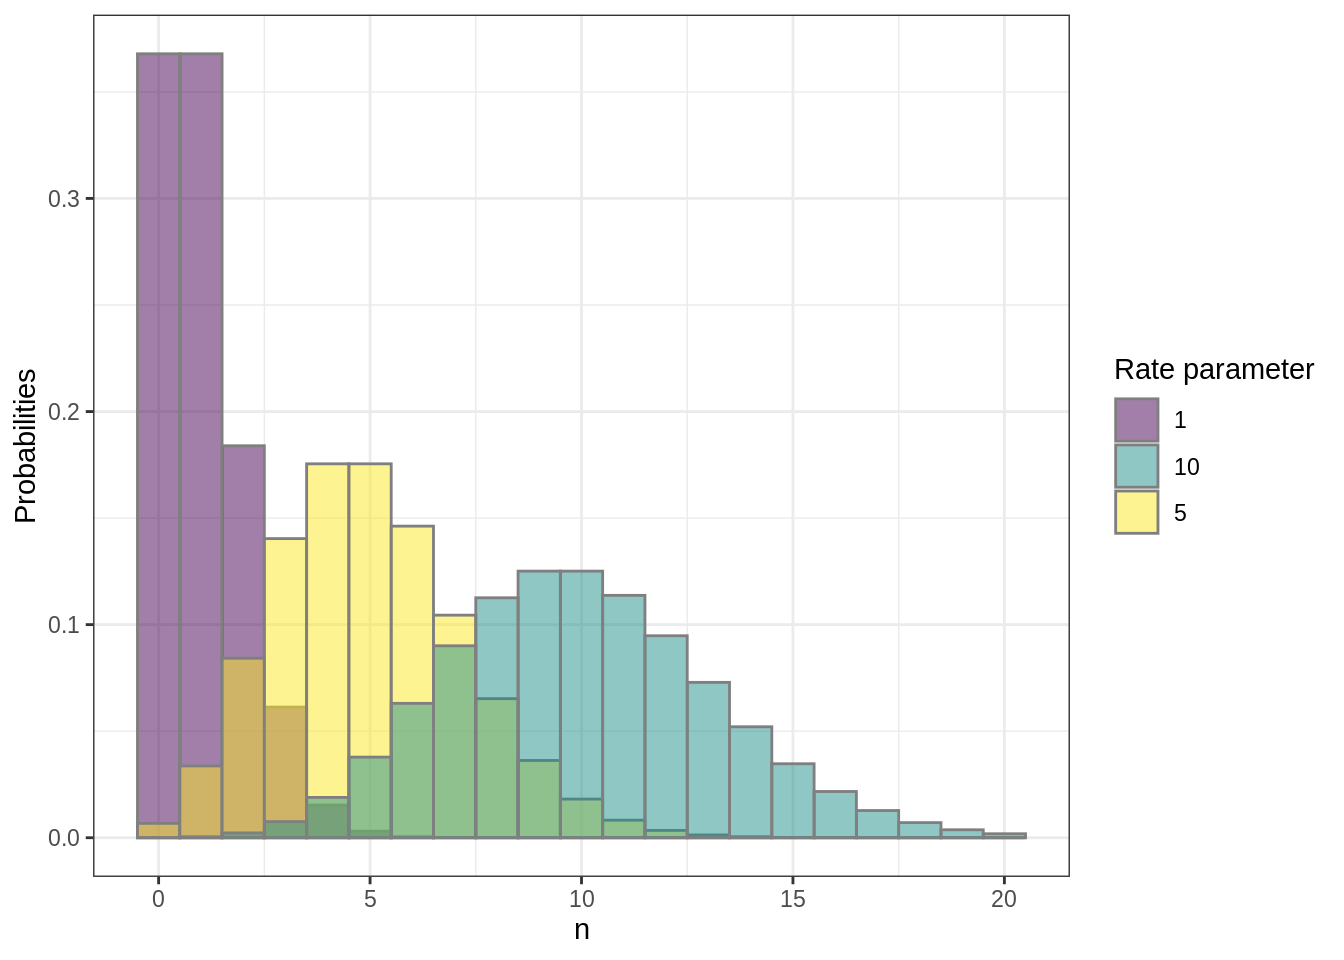
\includegraphics{783_biostats_files/figure-latex/unnamed-chunk-30-1.pdf}

This seems to be an okay estimate for a distribution of the heights (compare it to the histogram above). Say we want to find the probability that \(X\) the height of a randomly chosen participant is between \(178\) cm and \(190\) cm. We would do that by finding the area under the curve above.

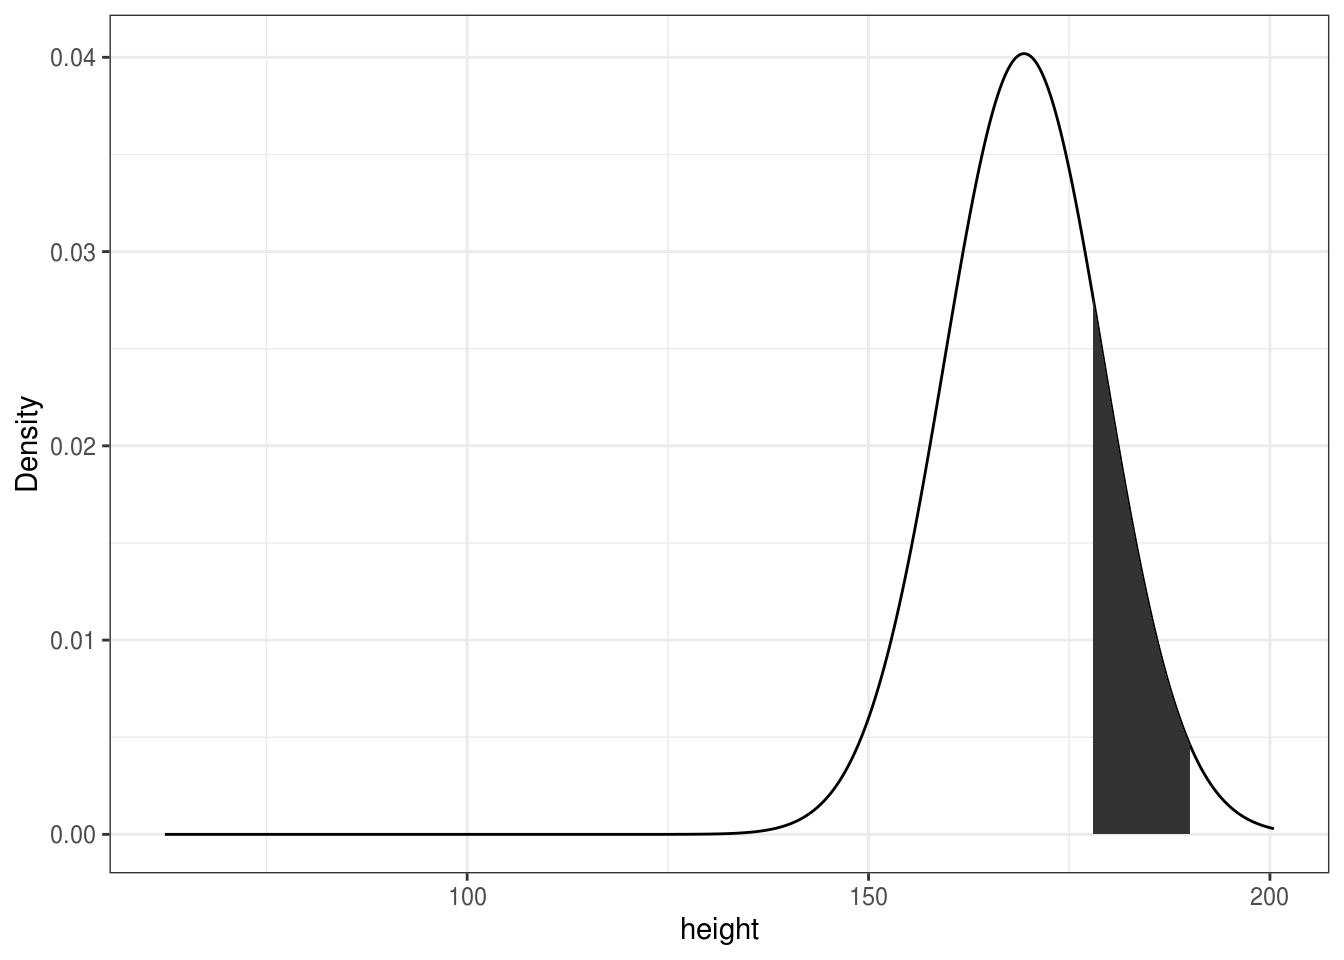
\includegraphics{783_biostats_files/figure-latex/unnamed-chunk-31-1.pdf}

This is not easy to do for us mortals (in this particular case, no closed form for the area exists!). Fortunately, some very smart people came up with some very smart ways to do this numerically -- that is, approximate the area with great precision. We'll simply let computers do this for us. In this particular case, the area is 0.174, or just about 17.4\%.

(\textbf{NOTE}: the rest of this subsection (\#random-variables) is not crucial for us, but is included for completeness. DO NOT panic if this seems super weird.)

There is one more thing we need to wrap our heads around: the probability of a continuous random variable being any single number is \(0\), no matter what number you choose. This might seem a weird -- how can the probability of observing a height of 6ft be \(0\) when we actually observe people that are 6ft tall?! I'll try to provide to explanations: an ``intuitive'' explanation, and one based on math. Run with whichever makes more sense to you (or just take my word for it!)

Remember when we first introduced the notion of continuous variables. We said that a \protect\hyperlink{continuous}{continuous variable} is a variable that can take an infinite (and actually uncountable) number of values. In the case of height, we also argued that even though it can technically be any value between 0ft and \href{https://www.guinnessworldrecords.com/world-records/tallest-man-ever}{8ft 11.1in}, we won't ever be able to measure it with \(100\%\) accuracy. So even though it \emph{seems} like we observe an individual that is 6ft tall that is not the exact height of said individual. Now, we could measure their height with greater accuracy, but no matter how accurate our tools are, we never get \(100\%\) accuracy.

From a mathematical point of view, consider a random variable \(X\) that follows the following distribution:

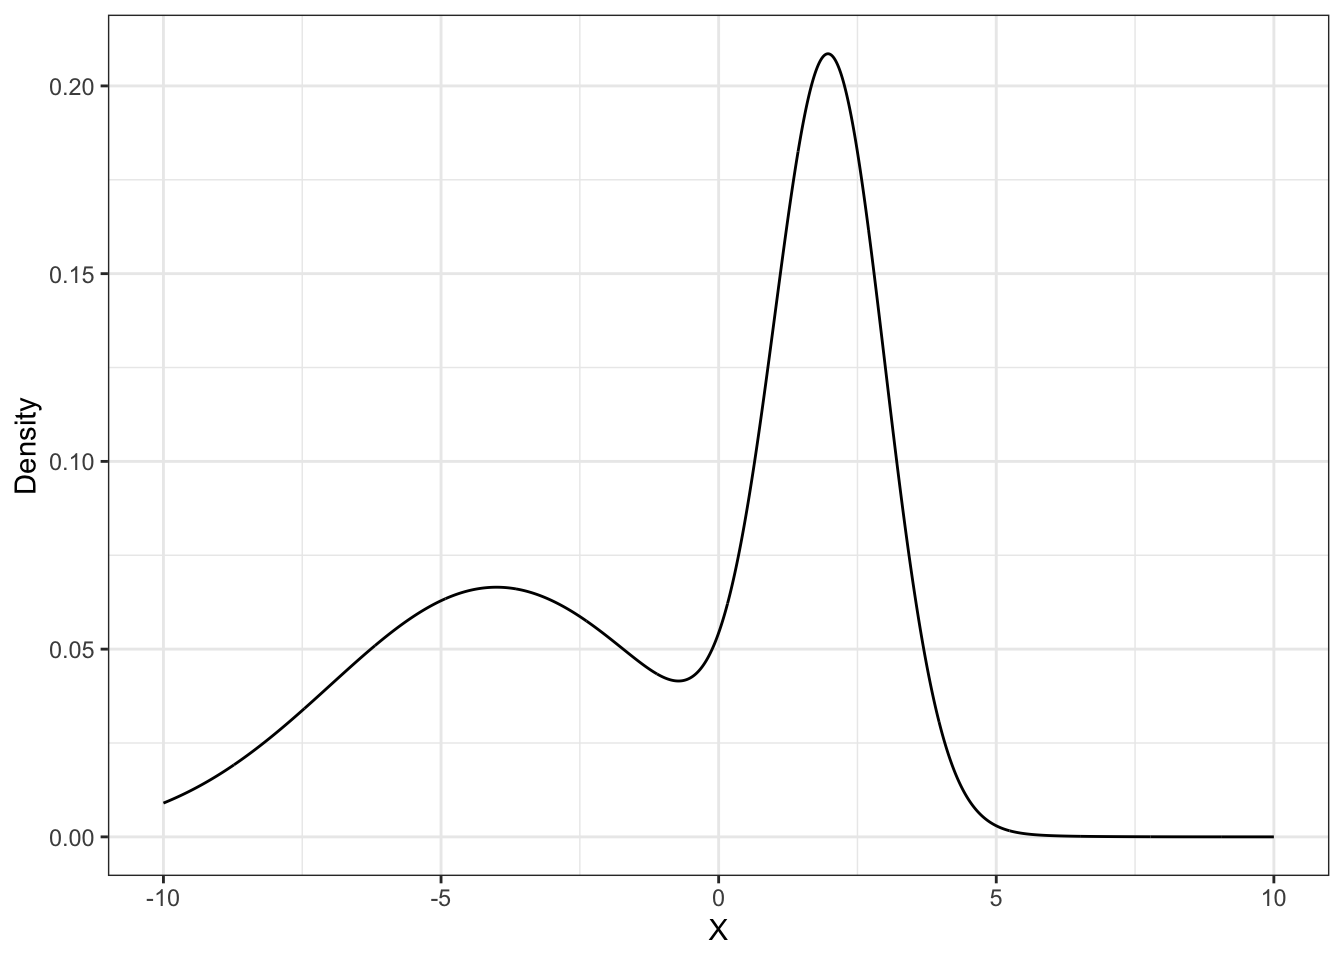
\includegraphics{783_biostats_files/figure-latex/unnamed-chunk-32-1.pdf}

Say we want to find the probability of \(X\) being between \(-1\) and \(2\). We would find that as the shaded area below, which turns out to be 0.317.

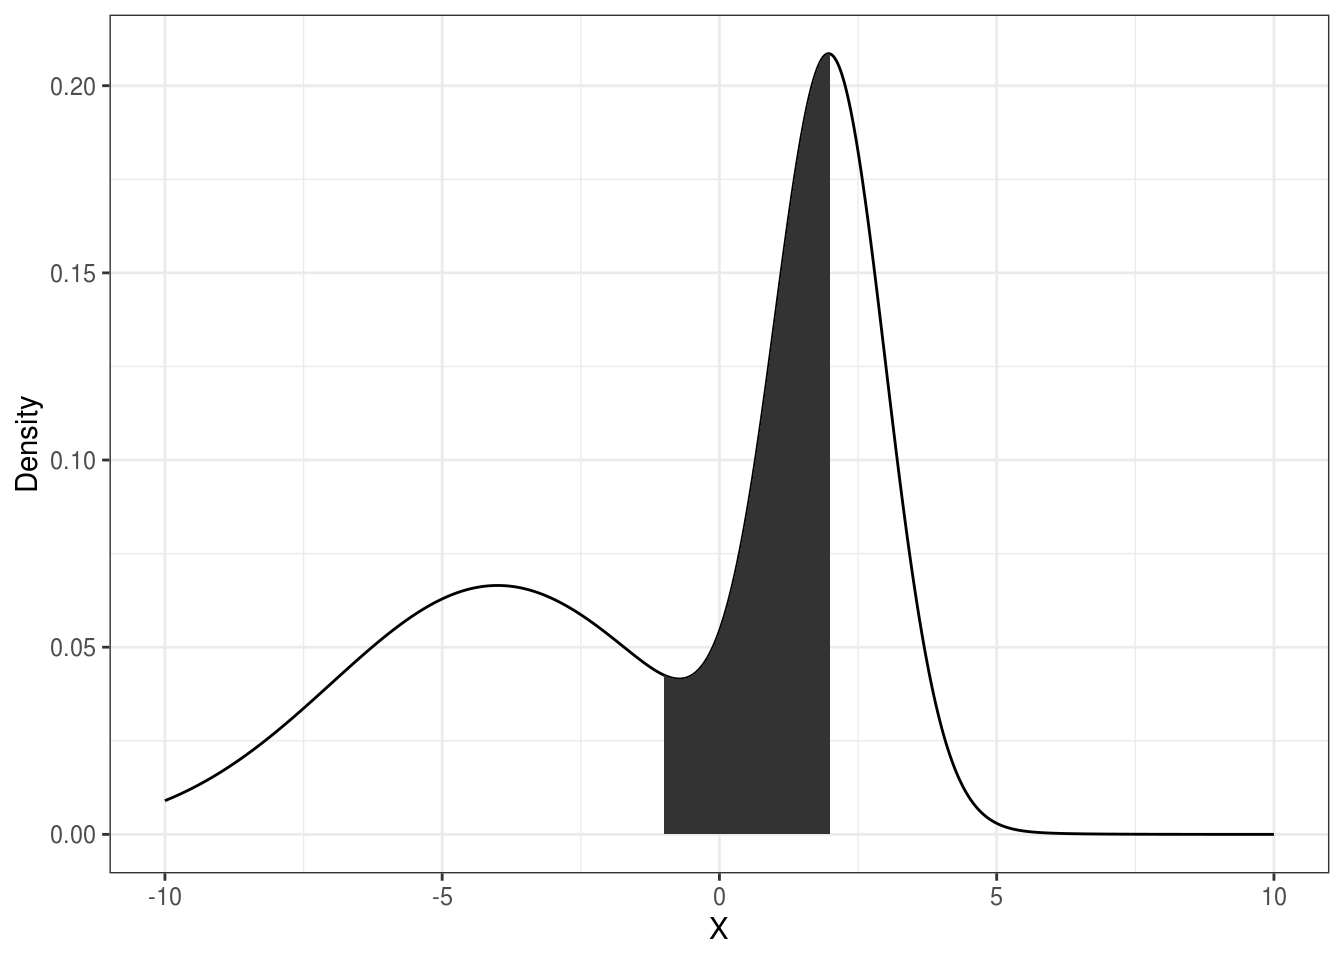
\includegraphics{783_biostats_files/figure-latex/unnamed-chunk-33-1.pdf}

Now imagine we want to find the area of \(X\) being between \(0\) and \(2\). This would be the shaded area below, which is 0.273

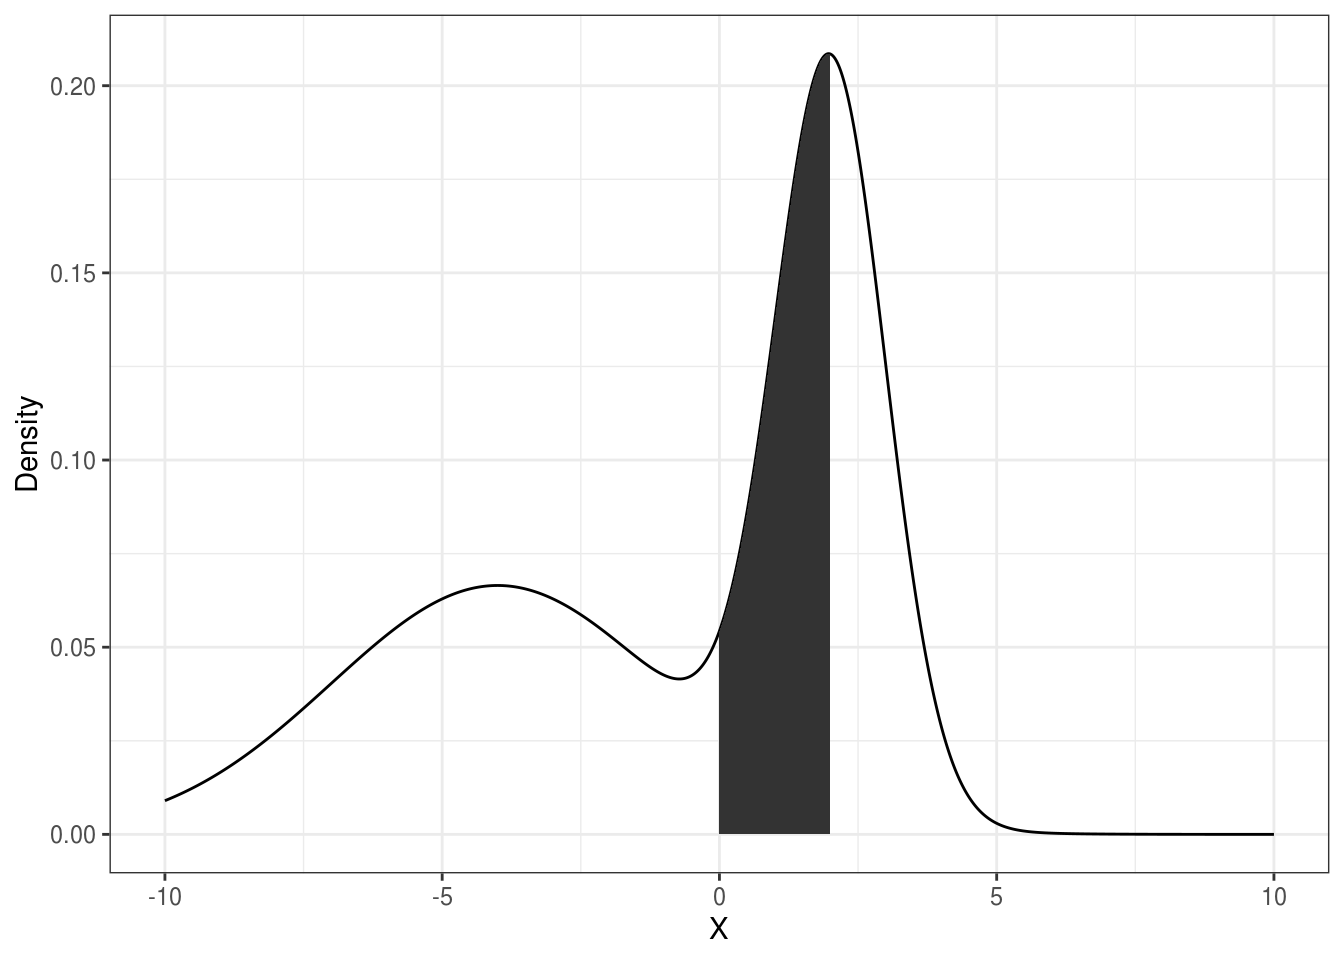
\includegraphics{783_biostats_files/figure-latex/unnamed-chunk-34-1.pdf}

How about the area between \(1\) and \(2\)? This is 0.183. Between \(1.5\) and \(2\): 0.101. Between \(1.9\) and \(2\): 0.021. Between \(1.995\) and \(2\): 0.001. As you can see, the closer we get to the ``interval'' \(2\) to \(2\), the smaller the area. In fact, if you take the limit, the area is \(0\).

\hypertarget{prop-of-RVs}{%
\section{Properties of Random Variables}\label{prop-of-RVs}}

When we talk about random variables, there is a great deal of uncertainty involved, since (by design) we do not know exactly what values the random variables will take after a conducted experiment. Similarly, we cannot be sure that repeating an experiment results in the same outcomes of the random variables simply since they are, as the name strongly implies, random. However, if we have some information about the random variable we're interested in, we can talk about some very important features of the random variable. The two we will talk about here are the \emph{expected value} and \emph{variance/standard deviation} of random variables.

These two concepts can be a bit hard to wrap ones head around at first, but as we talk about them over and over agian, hopefully you will realize that they are not as abstract as they might first seem.

\hypertarget{expected-values-of-random-variables}{%
\subsection{Expected Values of Random Variables}\label{expected-values-of-random-variables}}

The expected value of a random variable is, intuitively, the long run average. I.e. if we repeat an experiment \textbf{an infinite number of times}, we can determine the expected value of a random variable as the average of all the realizations of said random variable. As an example, if we consider the random variable \(X\) that is \(0\) if a coin flip comes up heads, and \(1\) if it comes up tails, we can imagine flipping a coin an infinite number of times, and calculating the average. The result would be that the expected value of \(X\) is \(0.5\). We write \(E(X) = 0.5\).

Note: the expected value is also often referred to as the \emph{mean} value.

For any discrete random variable where we know the distribution, we can find the expected value in the following way: \(E(X) = x_1 \cdot P(X = x_1) + ... + x_n P(X = x_n) = \sum_{i=1}^n x_i P(X = x_i)\).\footnote{\textbf{Note}: the symbol \(\sum\) simply means ``sum''. So, when we write \(\sum_{i=1}^n ...\) it simply means ``take the expression \ldots, plug in the value when \(i=1,2,3,...,n\), and then add them up''. Example: \(\sum_{i=1}^5 i = 1 + 2 + 3 + 4 + 5 = 15\). Example 2: if \(x_1 = 1, x_2 = 6, x_3 = -2.9\), then \(\sum_{i = 1}^3 x_i = 1 + 6 - 2.9 = 4.1\).}

\hypertarget{example-expected-value-of-discrete-random-variable}{%
\subsubsection{Example: expected value of discrete random variable}\label{example-expected-value-of-discrete-random-variable}}

Let \(X\) be a discrete random variable that can take the values \(1,2,6\), and \(12\). Let the probabilities of each outcome be as follows:

\begin{longtable}[]{@{}cc@{}}
\toprule
\begin{minipage}[b]{0.07\columnwidth}\centering
x\strut
\end{minipage} & \begin{minipage}[b]{0.14\columnwidth}\centering
P(X = x)\strut
\end{minipage}\tabularnewline
\midrule
\endhead
\begin{minipage}[t]{0.07\columnwidth}\centering
1\strut
\end{minipage} & \begin{minipage}[t]{0.14\columnwidth}\centering
0.2\strut
\end{minipage}\tabularnewline
\begin{minipage}[t]{0.07\columnwidth}\centering
2\strut
\end{minipage} & \begin{minipage}[t]{0.14\columnwidth}\centering
0.1\strut
\end{minipage}\tabularnewline
\begin{minipage}[t]{0.07\columnwidth}\centering
6\strut
\end{minipage} & \begin{minipage}[t]{0.14\columnwidth}\centering
0.6\strut
\end{minipage}\tabularnewline
\begin{minipage}[t]{0.07\columnwidth}\centering
12\strut
\end{minipage} & \begin{minipage}[t]{0.14\columnwidth}\centering
0.1\strut
\end{minipage}\tabularnewline
\bottomrule
\end{longtable}

Then we can calculate the expected value of \(X\):

\begin{align*}
  E(X) &= \sum_{i = 1}^4 x_i P(X = x_i) \\
       &= 1 \cdot P(X = 1) + 2 \cdot P(X = 2) + 6 \cdot P(X = 6) + 12 \cdot P(X = 12) \\
       &= 1\cdot 0.2 + 2\cdot 0.1 + 6 \cdot 0.6 + 12 \cdot 0.1 \\
       &= 5.2.
\end{align*}

So what does this mean? It means that if we perform an experiment that results in a realization of the random variable \(X\) many, many, many times, the average of all outcomes is going to be close to \(5.2\).

\begin{center}\rule{0.5\linewidth}{\linethickness}\end{center}

\hypertarget{example-expected-value-of-a-continuous-random-variable}{%
\subsubsection{Example: expected value of a continuous random variable}\label{example-expected-value-of-a-continuous-random-variable}}

In the continuous case, actually calculating the expected value isn't as easy as in the discrete case. Remember, when we specify a discrete distribution, we specify the probability of each possible outcome. When we specify a continuous distribution, we specify a curve over all the possible outcomes, and probabilities of specific events correspond to areas under the curve. This also means that it is impossible to use a formula like the one introduced for the discrete case above. Fortunately, the intuition is the same. The expected value is the long run average.

\begin{center}\rule{0.5\linewidth}{\linethickness}\end{center}

\hypertarget{rules-for-working-with-expected-values}{%
\subsubsection{Rules for working with expected values}\label{rules-for-working-with-expected-values}}

Sometimes, it is very beneficial to be able to transform a random variable, or combine several random variables, into a new one, and work with that new random variable. Fortunately, dealing with the expected value of a large number of such transformations is pretty simple.

First, let's imagine we have a random variable \(X\) with mean \(E(X)\), and another random variable \(Y\) with mean \(E(Y)\). Perhaps we are interested in the sum of the two, so we construct a new random variable \(Z = X + Y\).\footnote{Example: maybe we sent out a survey to a bunch of households asking for the income of each adult in the household (\(X\) and \(Y\)), and now we want to combine the two into a single total household income (\(Z = X + Y\)).} Finding the expected value of \(Z\) is really simple: \(E(Z) = E(X + Y) = E(X) + E(Y)\). In words: the expected value of a sum of random variables is simply the sum of expected values.

Another example: maybe we want to scale the outcome of the random variable \(X\) by a constant \(a\), and then consider the new random variable \(Y = a\cdot X\).\footnote{Example: maybe \(X\) is the total household income found from a survey in Europe where the currency is Euro. We want to compare this to our study of household incomes in the U.S., but to do so we have to convert from Euro to US Dollars. Here, \(X\) is the household income in Euro, \(a\) the exchange rate from Euro to US Dollars, and \(Y\) the household income in US Dollars.} Again, finding the expected value of the new random variable \(Y\) is really simple: \(E(Y) = E(aX) = a\cdot E(X)\).

One final thing I want to mention here: the expected value of a constant will always be the constant itself. Hopefully, this doesn't come as too much of a shock. The expected value is what we would \emph{expect} from a random variable. If something is constant, it means it never changes, so we \emph{expect} it to stay the same. So, if \(a\) is a constant, \(E(a) = a\). This can be combined with the first rule we talked about to give us that \(E(X + a) = E(X) + E(a) = E(X) + a\).

\hypertarget{variancestandard-deviation-of-random-variables}{%
\subsection{Variance/Standard Deviation of Random Variables}\label{variancestandard-deviation-of-random-variables}}

Where the expected value of a random variable tells us something about where the outcomes of the random variable tend to be located, the next measures we'll be looking at tell us something about how spread out the outcomes will be around the expected value.

\textbf{Note}: most textbooks handle the variance and standard deviations as two distinct things. I don't like that. They are virtually two sides of the same coin, and I will deliberately handle the two at the same time. My reasoning for this is that, at least in my head, these two measures try to convey the same message, but to two different audiences. I will elaborate on this later, but try to keep in mind that these two measures are almost the same.

The \emph{variance} of a random variable is a measure that tells us how much we expect the outcome of said random variable to vary from the expected value. As with the expected value, it is relatively simple to calculate this when we are dealing with simple discrete random variables. Let \(X\) be a discrete random variable with possible outcomes \(x_1, ..., x_n\), and the probability of \(x_i\) is \(P(X = x_i)\). Then the variance of \(X\) is \(\text{Var}(X) = \sum_{i=1}^n P(X = x_i)(x_i - E(X))^2\). At first glance, this can look a bit intimidating, so let's try to break it down to better understand what's going on:

\begin{enumerate}
\def\labelenumi{\arabic{enumi}.}
\tightlist
\item
  It actually has the form of an expected value, i.e.~it is a sum where each term is the product of the value of an outcome and the probability of that outcome. So, intuitively, this is not much different than an expected value, it's just an expected value of something else.
\item
  That ``something else'' is \((x_i - E(X))^2\). This is representative of the distance from the outcome \(x_i\) to the expected value\ldots{}
\item
  \ldots{} except, we square the distance. We do this because we want this measure to be representative of the variation of the data, and so we cannot allow positive and negative differences to cancel. Example: if we didn't square the differences, a random variable with possible outcomes \(1,2,3\) each with probability \(1/3\) would have variance \(0\), but clearly there is some variation in the potential outcomes -- not all observations are the same.
\end{enumerate}

So, loosely speaking, the variance is ``a measure of expected distances from observations to the expected value''.

\hypertarget{rules-for-working-with-variance}{%
\subsubsection{Rules for working with variance}\label{rules-for-working-with-variance}}

Working with the variance of random variables is not quite as simple as working with the expected value. This is due to the fact that the expected value is a simple average, whereas the variance is an average of squared differences. The result is the following set of rules: if \(X\) and \(Y\) are random variables, and \(a\) is some fixed constant, then

\begin{enumerate}
\def\labelenumi{\arabic{enumi}.}
\tightlist
\item
  \(\text{Var}(a\cdot X) = a^2 \text{Var}(X)\),
\item
  \(\text{Var}(a) = 0\),
\item
  if \(X\) and \(Y\) are independent: \(\text{Var}(X+Y) = \text{Var}(X) + \text{Var}(Y)\).
\end{enumerate}

Combining (1) and (3) above tells us that, if \(X\) and \(Y\) are independent, then

\begin{align*}
\text{Var}(X - Y) &= \text{Var}(X + (-Y)) \\
            &= \text{Var}(X) + \text{Var}(-Y) \\
            &= \text{Var}(X) + (-1)^2 \text{Var}(Y) \\
            &= \text{Var}(X) + \text{Var}(Y).
\end{align*}

Don't forget this!!

\hypertarget{so-what-about-that-standard-deviation}{%
\subsubsection{So what about that standard deviation?}\label{so-what-about-that-standard-deviation}}

So far we've talked about the variance, a bit about how to interpret it, and how to work with it for multiple random variables. But what about that other thing mentioned above, the standard deviation?

The standard deviation of a random variable is simply the square root of the variance: \(\text{SD}(X) = \sqrt{\text{Var}(X)}\). As we saw above, the variance has some nice mathematical properties, such as the fact that it is basically an expected value, and that (when \(X\) and \(Y\) are independent) \(\text{Var}(X + Y) = \text{Var}(X) + \text{Var}(Y)\). Neither hold for the standard deviation. We lose both because of the square root. However, it is also because of the square root that we like using the standard deviation in certain situation.

As mentioned, the variance is nice mathematically, but as soon as we make our way back from the beautiful haven that is the Land of Mathematics, and want to communicate our findings to collaborators or the rest of the world, the variance isn't great. Since we square all the differences, the unit of the variance is whatever unit your original measure was squared. Example: we might wish to estimate the height of adults in the SHOW data, and report it with some measure of uncertainty. We find that the average height is 66.06 inches, and the variance is 14.99\ldots{} \textsuperscript{inches}? This is hard to really grasp, and the number itself doesn't mean much to us. Is 22 inches\textsuperscript{2} a lot? We can't even really compare it to the mean because of the different units! The standard deviation fixes just that. It is still a measure of the ``expected'' variation, but it is measure on the original scale by taking the square root. So when we report a mean height of 66.06 inches with a standard deviation of 3.87 inches, this all of a sudden makes much more sense intuitively.

The moral of the story: both the variance and the standard deviation have a role in the world of statistics, but at different stages. The variance is very useful in the more mathematical parts of the field, while the standard deviation is easier to interpret. Luckily, going from one to the other is simple: \(\text{Var}(X) = \text{SD}(X)^2\) and \(\text{SD}(X) = \sqrt{\text{Var}(X)}\). Therefore, if you ever have one, you practically have both. Don't forget this, as it is a common mistake to plug in the variance to equations where it should have been the standard deviation, and vice versa.

\hypertarget{things-to-remember-when-working-with-random-variables}{%
\subsection{Things to remember when working with random variables}\label{things-to-remember-when-working-with-random-variables}}

When working with random variables, \(X\) and \(Y\), these are the important rules:

\begin{enumerate}
\def\labelenumi{\arabic{enumi}.}
\tightlist
\item
  \(E(X + Y) = E(X) + E(Y)\),
\item
  if \(a\) is some fixed number, \(E(a\cdot X) = a\cdot E(X)\),
\item
  if \(a\) is some fixed number, \(\text{Var}(a \cdot X) = a^2 \text{Var}(X)\),
\item
  \textbf{IF} \(X\) and \(Y\) are independent, \(\text{Var}(X + Y) = \text{Var}(X) + \text{Var}(Y)\),
\item
  \textbf{IF} \(X\) and \(Y\) are independent, \(\text{Var}(X - Y) = \text{Var}(X) + \text{Var}(Y)\).
\end{enumerate}

Things people often forget:

\begin{enumerate}
\def\labelenumi{\arabic{enumi}.}
\tightlist
\item
  \(E(X\cdot Y) \neq E(X)E(Y)\),
\item
  \(E\left(\frac{X}{Y}\right) \neq \frac{E(X)}{E(Y)}\),
\item
  \(\text{Var}(X+Y) \neq \text{Var}(X) + \text{Var}(Y)\) if \(X\) and \(Y\) are not independent,
\item
  \(\text{Var}(X - Y) \neq \text{Var}(X) - \text{Var}(Y)\),
\item
  \(\text{SD}(X + Y) \neq \text{SD}(X) + \text{SD}(Y)\), even when \(X\) and \(Y\) are independent.
\end{enumerate}

\hypertarget{a-few-important-distributions}{%
\section{A Few Important Distributions}\label{a-few-important-distributions}}

\hypertarget{the-bernoulli-distribution}{%
\subsection{The Bernoulli Distribution}\label{the-bernoulli-distribution}}

In example \ref{examples-random-variables} above, we consider flipping a coin. Such an experiment, i.e.~one with only two possible outcomes, is often referred to as a \emph{Bernoulli experiment}, and the random variable \(X\) is referred to as a \emph{Bernoulli random variable}. The ``probability of success'' (you get to pick your favorite outcome as a success) is often denoted \(p\). As a shorthand for such a random variable, we write \(X \sim \text{Bernoulli}(p)\), which is read as ``\(X\) follows a Bernoulli distribution with probability parameter \(p\)'' or ``\(X\) is Bernoulli distributed with parameter \(p\)''. Phrases like these can sometimes sound scary and complex, but all it means is that the random variable \(X\) can only take on two different outcomes, and the probability of \(X\) being one of the two outcomes is \(p\), the probability of it being the other is \(1-p\). (Important note: remember that the sum of all probabilities has to be \(1\), so if the probability of one outcome is \(p\), and there are only two possible outcomes, then the probability of the other outcome must be \(1-p\). This way of thinking is something we will use over and over again.)

Using the properties discussed in section \ref{prop-of-RVs}, we can calculate the expected value and variance of a Bernoulli random variable. Simply using the definitions, we see that

\[
  E(X) = \sum_{i=1}^2 x_i \cdot P(X = x_i) = 0 \cdot P(X = 0) + 1 \cdot P(X = 1) = p,
\]

and

\begin{align*}
  \text{Var}(X) &= \sum_{i=1}^2 P(X = x_i) \cdot (x_i - E(X))^2 \\
          &= P(X = 0)\cdot (0 - p)^2 + P(X = 1)\cdot (1 - p)^2 \\
          &= (1 - p)\cdot p^2 + p\cdot (1 - p)^2 \\
          &= (1-p)\cdot(p^2 + p\cdot(1-p)) \\
          &= (1-p)\cdot(p^2 + p - p^2) \\
          &= (1-p)\cdot p.
\end{align*}

So it is actually rather simple to find the expected value and variance of a Bernoulli random variable, if we know the probability of success (\(p\)).

\hypertarget{the-binomial-distribution}{%
\subsection{The Binomial Distribution}\label{the-binomial-distribution}}

Often times we are interested in things that can be viewed as a sum of Bernoulli random variables. Let's say we have \(n\) independent (i.e.~the outcome of one doesn't say anything about the rest) Bernoulli random variables (\(X_1\), \(X_2\), \ldots, \(X_n\)), all with probability of success \(p\), and are interested in the sum of those \(n\) variables \(Y = X_1 + X_2 + ... + X_n\). For this to make sense, we let \(X_i\) be \(1\) if the corresponding ``experiment'' is a success, and \(0\) if it is a failure. Now, we can think of the random variable \(Y\) as either (1) the sum of independent Bernoulli random variables, or (2) the number of successes among \(n\) independent trials with binary outcomes. It is this latter interpretation that makes the random variable \(Y\) interesting.

When a random variable is the sum of \(n\) independent Bernoulli random variables all with probability of success \(p\), we say that \(Y\) follows a Binomial distribution with size \(n\) and probability of success \(p\). We write \(Y \sim \text{Binomial}(n,p)\).

Let's think for a second about what possible values \(Y\) can take. If all \(n\) Bernoulli experiments happen to come out as failures, then all \(X_i\)'s are \(0\)'s, and so \(Y\) will also be \(0\). The other extreme is if all \(n\) Bernoulli experiments are successes, then all \(X_i\)'s are \(1\)'s, and \(Y\) will be the sum of \(n\) \(1\)'s, so \(Y\) will be \(n\). These are simply the two extremes - any number of the \(X_i\)'s can be \(1\)'s, so \(Y\) can end up being any integer between \(0\) and \(n\), both included. The most likely scenarios are the integers closest to the middle.

Since \(Y\) is simply a sum of very simple random variables, namely Bernoulli random variables, we can with very simple tools dive deeper, and try to explore what the distribution of a Binomial random variable looks like. We can find the expected value and variance, and the probability of all possible outcomes. There are two ways of doing this: (1) do the math, or (2) flip \(n\) coins an infinite number of times and see how often the number of heads is each of the possible outcomes. Let's start with the latter.

Since it's impossible to flip \(n\) coins (for what is \(n\)?), we have to pick a real integer. Let's pick \(10\). Similarly, it's impossible to flip \(10\) coins an infinite number of times, so let's just do it a bunch of times (i.e.~\(`r `\)). What we are about to do is repeat an experiment (flip \(10\) coins) many, many (\(50000\)) times. The first time we perform this experiment, we see T,H,H,T,H,T,T,H,H,H. When we translate this to \(0\) and \(1\), it looks like 0,1,1,0,1,0,0,1,1,1. So, the value of the binomial variable \(Y\) is 6, since this is the number of heads. Rinse and repeat. The results of all \(10\) experiments are shown in the table below.

\hypertarget{htmlwidget-114adde79a5d99c64891}{}

Now we can get a pretty good estimate of the distribution of \(Y\). Recall, the distribution of a random variable is simply the probabilities of each possible outcome. The probability of a particular outcome, say \(Y = 2\), is the long run proportion of experiments that result in that outcome. So, \(P(Y = 2) = \frac{\text{number of experiments with } Y = 2}{\text{number of experiments}} = \frac{2252}{\ensuremath{5\times 10^{4}}} = 0.04504\). If we do this for every possible value of \(Y\), we get something that looks like the following:

\begin{longtable}[]{@{}ccc@{}}
\toprule
\begin{minipage}[b]{0.06\columnwidth}\centering
y\strut
\end{minipage} & \begin{minipage}[b]{0.34\columnwidth}\centering
\# experiments with Y = y\strut
\end{minipage} & \begin{minipage}[b]{0.30\columnwidth}\centering
Estimated Probability\strut
\end{minipage}\tabularnewline
\midrule
\endhead
\begin{minipage}[t]{0.06\columnwidth}\centering
0\strut
\end{minipage} & \begin{minipage}[t]{0.34\columnwidth}\centering
56\strut
\end{minipage} & \begin{minipage}[t]{0.30\columnwidth}\centering
0.00112\strut
\end{minipage}\tabularnewline
\begin{minipage}[t]{0.06\columnwidth}\centering
1\strut
\end{minipage} & \begin{minipage}[t]{0.34\columnwidth}\centering
460\strut
\end{minipage} & \begin{minipage}[t]{0.30\columnwidth}\centering
0.0092\strut
\end{minipage}\tabularnewline
\begin{minipage}[t]{0.06\columnwidth}\centering
2\strut
\end{minipage} & \begin{minipage}[t]{0.34\columnwidth}\centering
2252\strut
\end{minipage} & \begin{minipage}[t]{0.30\columnwidth}\centering
0.045\strut
\end{minipage}\tabularnewline
\begin{minipage}[t]{0.06\columnwidth}\centering
3\strut
\end{minipage} & \begin{minipage}[t]{0.34\columnwidth}\centering
5928\strut
\end{minipage} & \begin{minipage}[t]{0.30\columnwidth}\centering
0.119\strut
\end{minipage}\tabularnewline
\begin{minipage}[t]{0.06\columnwidth}\centering
4\strut
\end{minipage} & \begin{minipage}[t]{0.34\columnwidth}\centering
10267\strut
\end{minipage} & \begin{minipage}[t]{0.30\columnwidth}\centering
0.205\strut
\end{minipage}\tabularnewline
\begin{minipage}[t]{0.06\columnwidth}\centering
5\strut
\end{minipage} & \begin{minipage}[t]{0.34\columnwidth}\centering
12396\strut
\end{minipage} & \begin{minipage}[t]{0.30\columnwidth}\centering
0.248\strut
\end{minipage}\tabularnewline
\begin{minipage}[t]{0.06\columnwidth}\centering
6\strut
\end{minipage} & \begin{minipage}[t]{0.34\columnwidth}\centering
10214\strut
\end{minipage} & \begin{minipage}[t]{0.30\columnwidth}\centering
0.204\strut
\end{minipage}\tabularnewline
\begin{minipage}[t]{0.06\columnwidth}\centering
7\strut
\end{minipage} & \begin{minipage}[t]{0.34\columnwidth}\centering
5820\strut
\end{minipage} & \begin{minipage}[t]{0.30\columnwidth}\centering
0.116\strut
\end{minipage}\tabularnewline
\begin{minipage}[t]{0.06\columnwidth}\centering
8\strut
\end{minipage} & \begin{minipage}[t]{0.34\columnwidth}\centering
2089\strut
\end{minipage} & \begin{minipage}[t]{0.30\columnwidth}\centering
0.0418\strut
\end{minipage}\tabularnewline
\begin{minipage}[t]{0.06\columnwidth}\centering
9\strut
\end{minipage} & \begin{minipage}[t]{0.34\columnwidth}\centering
464\strut
\end{minipage} & \begin{minipage}[t]{0.30\columnwidth}\centering
0.00928\strut
\end{minipage}\tabularnewline
\begin{minipage}[t]{0.06\columnwidth}\centering
10\strut
\end{minipage} & \begin{minipage}[t]{0.34\columnwidth}\centering
54\strut
\end{minipage} & \begin{minipage}[t]{0.30\columnwidth}\centering
0.00108\strut
\end{minipage}\tabularnewline
\bottomrule
\end{longtable}

We see that the most probable outcomes are around the middle (4,5,6) with proportions above 0.20.

We can display this using a histogram. Even though this is actually a discrete random variable, the histogram can still be used to display the distribution, just make sure the binwidths are adjusted appropriately (in this case, width of \(1\) is good since that ensures each bar corresponds to one possible outcome).

\hypertarget{htmlwidget-628b959b19de1aaa1209}{}

When viewing this, the probability of a given outcome can be interpreted as the area of the corresponding bar divided by the total area.

As mentioned earlier, the distribution of a binomial random variable can also be calculated mathematically. We won't go into the details here, but I will leave you with the formulat: \(P(Y = k) = {n \choose k}p^k (1-p)^{n-k}\)\footnote{\({n \choose k}\) is read as ``n choose k'' and is the number of ways you can choose \(k\) elements from \(n\) elements. For example, the number of ways you can pick \(2\) balls out of a basked of \(3\) different balls is \({3 \choose 2}\). It can be calculated as \({n \choose k} = \frac{n!}{k!(n-k)!}\), where \(n!\) (``\(n\) factorial'') is \(n\cdot (n-1) \cdot (n-2) \cdot ... \cdot 2 \cdot 1\). By definition, \(0! = 1\).}. Take a look at the calculated probabilities below, and compare them to the estimates we got by flipping \(10\) coins \(50000\) times.

As mentioned earlier, the distribution of a binomial random variable can also be calculated mathematically. We won't go into the details here, but I will leave you with the formula: \(P(Y = k) = {n \choose k}p^k (1-p)^{n-k}\)\footnote{\({n \choose k}\) is read as ``n choose k'' and is the number of ways you can choose \(k\) elements from \(n\) elements. For example, the number of ways you can pick \(2\) balls out of a basked of \(3\) different balls is \({3 \choose 2}\). It can be calculated as \({n \choose k} = \frac{n!}{k!(n-k)!}\), where \(n!\) (``\(n\) factorial'') is \(n\cdot (n-1) \cdot (n-2) \cdot ... \cdot 2 \cdot 1\). By definition, \(0! = 1\).}. Take a look at the calculated probabilities below, and compare them to the estimates we got by flipping \(10\) coins \(50000\) times.

\hypertarget{htmlwidget-b11304a5a5b59d838d47}{}

Pretty close!

As mentioned, the expected value is basically the long run average. So, if we calculate the average of all outcomes of \(Y\) we get a good estimate of what the expected value of \(Y\) is. Similarly, the variance of the outcomes is a good estimate of the variance of the random variable \(Y\). From the data, \(\bar{y} = 4.98496\) and \(s_Y^2 = 2.4813434\). Remember those two numbers.

If we use the rules of expectation and variance from the previous section, we can find the exact expected value and variance of a binomial random variable with size \(n\) and probability of success \(p\). Since \(Y \sim \text{Binomial}(n,p)\) if \(Y = X_1 + ... + X_n\), where \(X_i \sim \text{Bernoulli}(p)\) and all \(X_i\)'s are independent, we have that

\begin{align*}
  E(Y) &= E(X_1 + ... + X_n) && \\
       &= E(X_1) + ... + E(X_n) && \\
       &= p + ... p && (E(X_i) = p \text{ since } X_i \sim \text{Bernoulli}(p)) \\
       &= n\cdot p, &&
\end{align*}

and

\begin{align*}
  \text{Var}(Y) &= \text{Var}(X_1 + ... + X_n) && \\
          &= \text{Var}(X_1) + ... + \text{Var}(X_n) && (\text{since all } X_i's \text{ are independent}) \\
          &= p\cdot(1-p) + ... + p\cdot(1-p) && (\text{since } X_i \sim \text{Bernoulli}(p)) \\
          &= n\cdot p \cdot (1-p). &&
\end{align*}

These two equations really emphasize that a Binomial random variable is really just \(n\) Bernoulli's: notice how both the expected value and the variance is \(n\) times that of a single Bernoulli random variable!

Now let's calculate the expected value and variance of our little experiment. We flip a coin \(10\) times. The probability of success is \(0.5\). So, \(Y \sim \text{Binomial}(10, 0.5)\), and therefore \(E(Y) = 10 \cdot 0.5 = 5\), and \(\text{Var}(Y) = 10 \cdot 0.5 \cdot (1-0.5) = 2.5\). Remember what we got for the expected value and variance? Numbers very close to these.

\hypertarget{normal-distribution}{%
\subsection{Normal Distribution}\label{normal-distribution}}

The normal distribution is most definitely the most important distribution we will discuss in this class for one reason: The Central Limit Theorem. We'll get back to what this is later, but first let's try to become familiar with the normal distribution.

In contrast to the Bernoulli and Binomial distributions, the normal distribution is a continuous distribution, and therefore it is specified by a curve.

The normal distribution density is specified by two parameters. The first specifies the mean of the distribution (and is therefore called the \emph{mean} or \emph{location} paramater). We often use \(\mu\) to denote the mean of a normal distribution, or \(\mu_X\) if we want to really stress that we are talking about the mean of the random variable \(X\)\footnote{very useful when we are working with multiple random variables, as we will see in a second}. The second parameter specifies the variance of the distribution. We often use \(\sigma^2\) to denote this, or \(\sigma_X^2\). This is rather convenient, as when we then talk about the standard deviation, it is simply \(\sigma\). The mean parameter can really be any real number, while the variance has to be positive. If \(X\) follows a normal distribution with mean \(\mu\) and variance \(\sigma^2\), we write \(X \sim N(\mu, \sigma^2)\).

So what does this curve actually look like? It's a bell curve that is centered at the mean \(\mu\) and the shape/width is controlled by the variance \(\sigma^2\). Below are a few examples. The first figure shows varying means, the second varying variances.

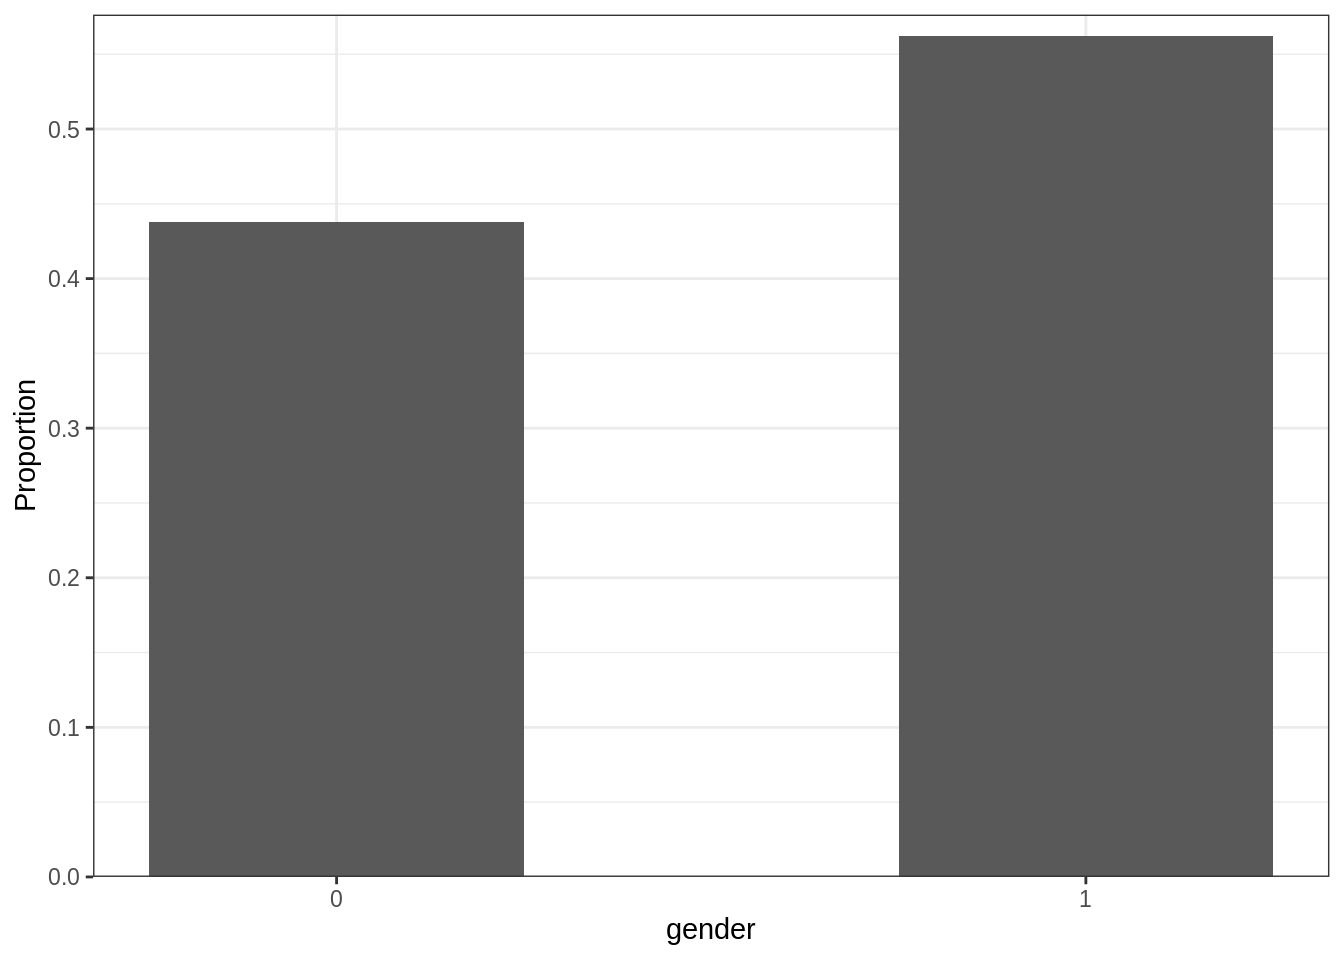
\includegraphics{783_biostats_files/figure-latex/unnamed-chunk-40-1.pdf}

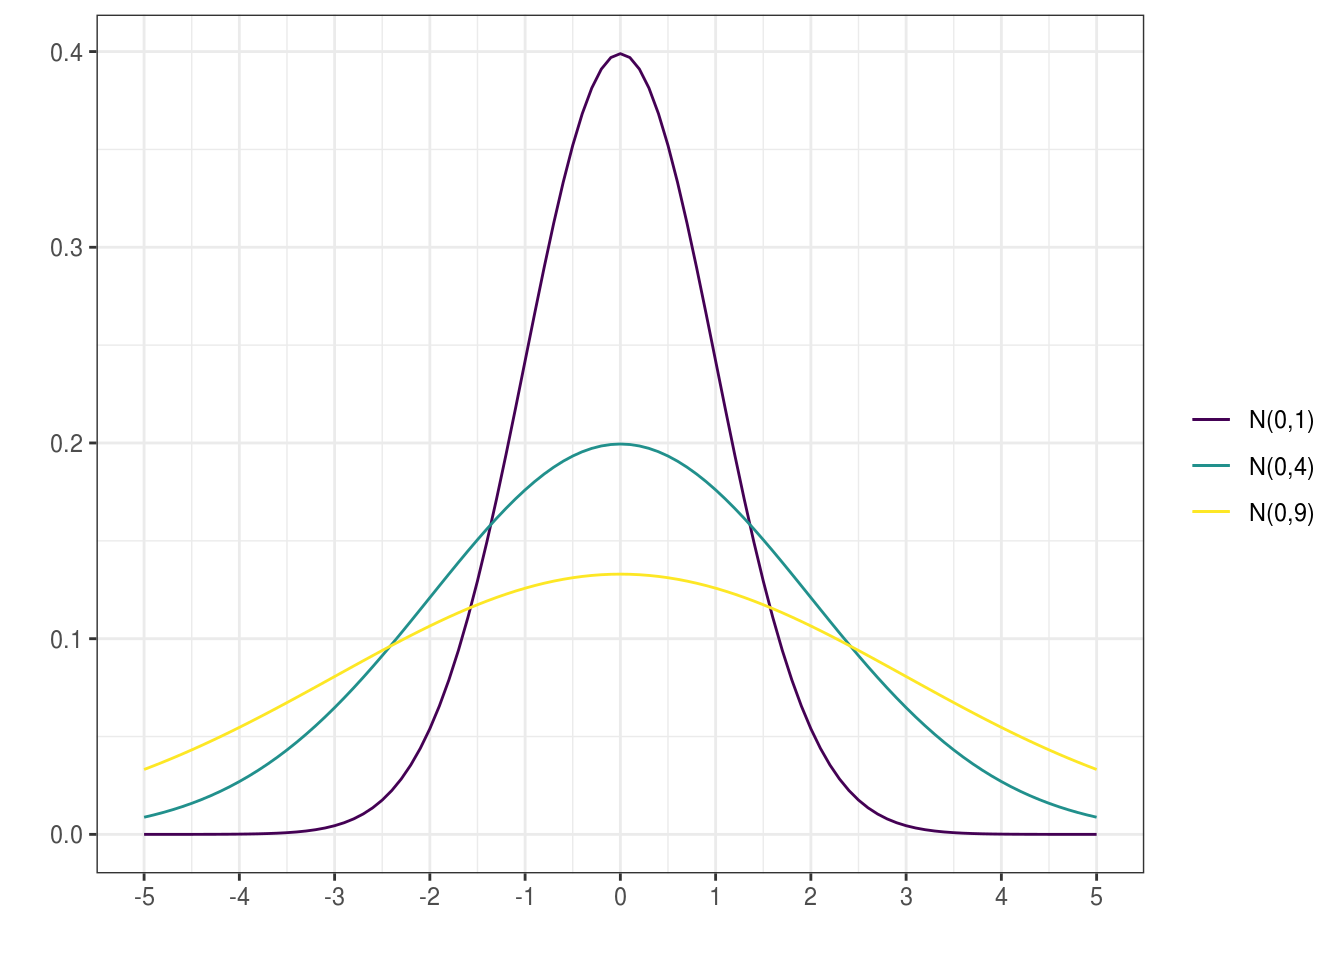
\includegraphics{783_biostats_files/figure-latex/unnamed-chunk-41-1.pdf}

As the names of the parameters suggest, the actual expected value and variance of a random variable that is normally distributed, \(X \sim N(\mu, \sigma^2)\), is simply \(\mu\) and \(\sigma^2\), respectively.

\hypertarget{lin-comb-normals}{%
\subsubsection{Linear Combination of Normal with Constants}\label{lin-comb-normals}}

One really neat property of the normal distribution is that if you add a constant number, \(a\), to a random variable you again get something that is normally distributed. Similarly, if you multiply by a constant you get back something that is still normally distributed. The exact normal distribution can easily be specified (recall: to specify a normal distribution, we need to find the mean and variance). For completeness, let's do this. If \(X \sim N(\mu, \sigma^2)\), then \(Y_1 = X+a\) and \(Y_2 = a\cdot X\) are also normally distributed. Using the properties of expected value and variance from section \ref{prop-of-RVs}, we get that

\begin{align*}
  E(Y_1) &= E(X+a) = E(X) + a = \mu + a, \\
  E(Y_2) &= E(a\cdot X) = a E(X) = a\cdot \mu,
\end{align*}

and

\begin{align*}
  \text{Var}(Y_1) &= \text{Var}(X+a) = \text{Var}(X) = \sigma^2, \\
  \text{Var}(Y_2) &= \text{Var}(a\cdot X) = a^2 \text{Var}(X) = a^2 \sigma^2.
\end{align*}

So \(X + a \sim N(\mu + a, \sigma^2)\), and \(a\cdot X \sim N(a\cdot \mu, a^2 \sigma^2)\).

One particular case of the normal distribution plays an important role in much of statistics, and is therefore been named the Standard Normal Distribution. For historic reasons, we often use \(Z\) to denote the standard normal distribution, which is simply a normal distribution with mean \(0\) and variance \(1\). I.e. \(Z \sim N(0,1)\). One reason why this is important is that it provides sort of a baseline that we can always revert to. Whenever you are working with a normal distribution, you can use the rules above to get the standard normal. If \(X \sim N(\mu, \sigma^2)\), then \(\frac{X-\mu}{\sigma} = Z \sim N(0,1)\). Why? As we just discussed, adding a constant to a normal random variable results in something normal. \(X-\mu\) is simply adding \(-\mu\) to \(X\), so this is still normal. We also saw that multiplying by a constant is still normal, so since \(\frac{X-\mu}{\sigma}\) is simply multiplying \(X-\mu\) by \(\frac{1}{\sigma}\), we have that \(\frac{X-\mu}{\sigma}\) is a normal random variable. We can find it's mean and variance using the rules we've learned, and get that \(E\left(\frac{X - \mu}{\sigma}\right) = \frac{E(X) - \mu}{\sigma} = 0\), and \(\text{Var}\left(\frac{X - \mu}{\sigma}\right) = \frac{\text{Var}(X)}{\sigma^2} = 1\), so \(\frac{X-\mu}{\sigma} = Z \sim N(0,1)\).

I want to reiterate the procedure of standardizing. Take a Normally distributed random variable, subtract its mean, and divide by the standard deviation will result in a new random variable that follows the standard normal distribution: \(\frac{X - E(X)}{\text{SD}(X)} \sim N(0,1)\).

\hypertarget{sum-of-independent-normals}{%
\subsubsection{Sum of (Independent) Normals}\label{sum-of-independent-normals}}

Another really important and useful property of the normal distribution is that if you have two normally distributed variables, \(X \sim N(\mu_X, \sigma_X^2)\) and \(Y \sim N(\mu_Y, \sigma_Y^2)\), then the sum of the two, \(X + Y\), is also a normally distributed random variable.

The mean parameter of this newly created random variable is always easy to find: \(E(X + Y) = E(X) + E(Y) = \mu_X + \mu_Y\). The variance is, in general a bit harder, except if the two are independent of each other. In this case \(\text{Var}(X + Y) = \text{Var}(X) + \text{Var}(Y) = \sigma_X^2 + \sigma_Y^2\). So, if \(X\) and \(Y\) are independent, then \(X + Y \sim N(\mu_X + \mu_Y, \sigma_X^2 + \sigma_Y^2)\).

Combining this with the rules stated above, we get that \(X - Y\) is normally distributed as well, since \(X - Y = X + (-Y)\), and both \(X\) and \(-Y\) are normally distributed. More applications of the rules give us \(X - Y \sim N(\mu_X - \mu_Y, \sigma_X^2 + \sigma_Y^2)\). (\textbf{NOTE}: we DO NOT subtract the variances.)

\hypertarget{some-exploration-through-simulations}{%
\subsubsection{Some Exploration through Simulations}\label{some-exploration-through-simulations}}

To illustrate the properties presented in the two previous sections, let us take a look at some simulated data. Let \(X \sim N(-0.5, 1)\) and \(Y \sim N(1, 1.5)\). I.e. \(X\) and \(Y\) follow these two distributions:

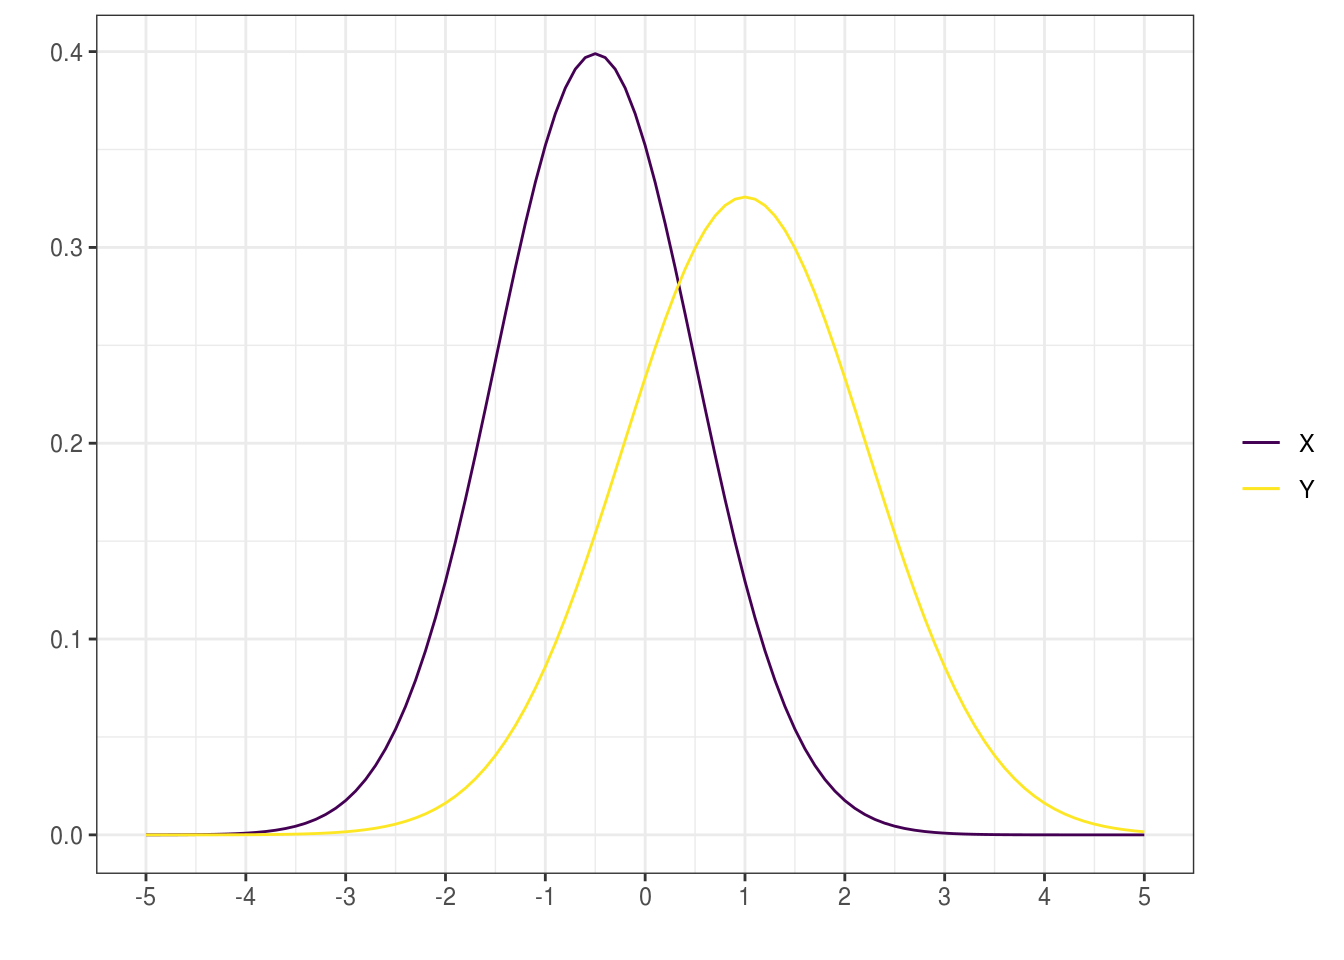
\includegraphics{783_biostats_files/figure-latex/unnamed-chunk-43-1.pdf}

Now, let's say we're actually interested in \(W = X - Y\). That is, we perform an experiment, observe a realization of \(X\) and \(Y\), and then create a realization of \(W\) as \(w = x - y\). The first experiment results in \(x = 1.5653, y = 0.7306\), and so \(w = x - y = 0.8347\). We repeat this experiment many, many (\(\ensuremath{10^{4}}\)) times. This enables us to take a look at histograms of the outcomes of \(X\), \(Y\), and \(W\), and we calculate the observed averages and variances so that we can compare with our theoretical expectations.

So, first of all: do \(X\) and \(Y\) actually match the distributions we wanted them to come from? Below are histograms of the outcomes with the distributions overlayed. Notice how closely the histograms follow the curves. It definitely seems that the outcomes of \(X\) and \(Y\) indeed come from the respective normal distributions.

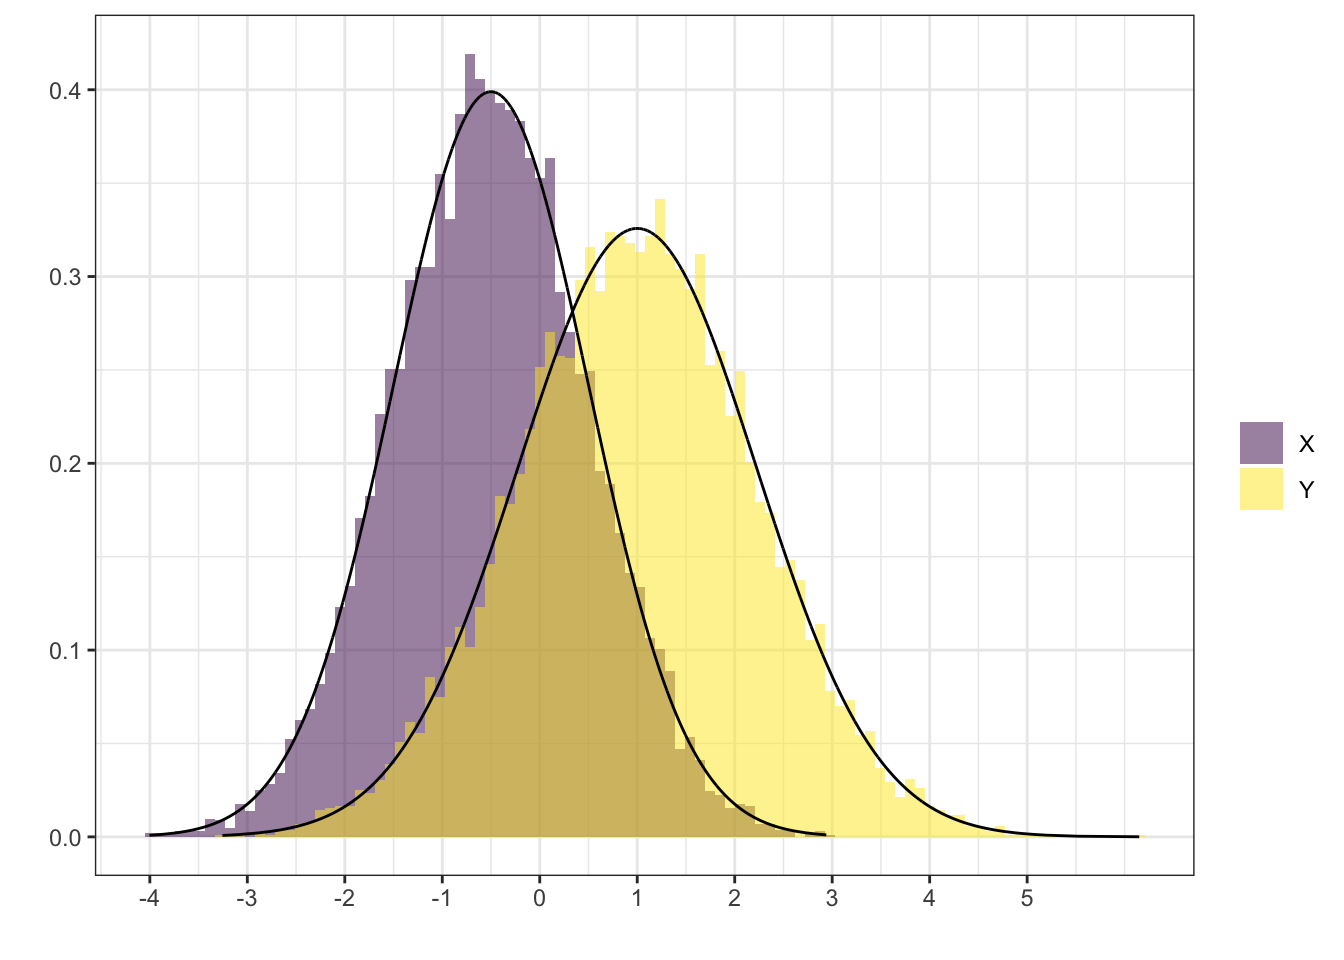
\includegraphics{783_biostats_files/figure-latex/unnamed-chunk-44-1.pdf}

Now, let us take a look at the difference between the two, i.e.~\(W\).

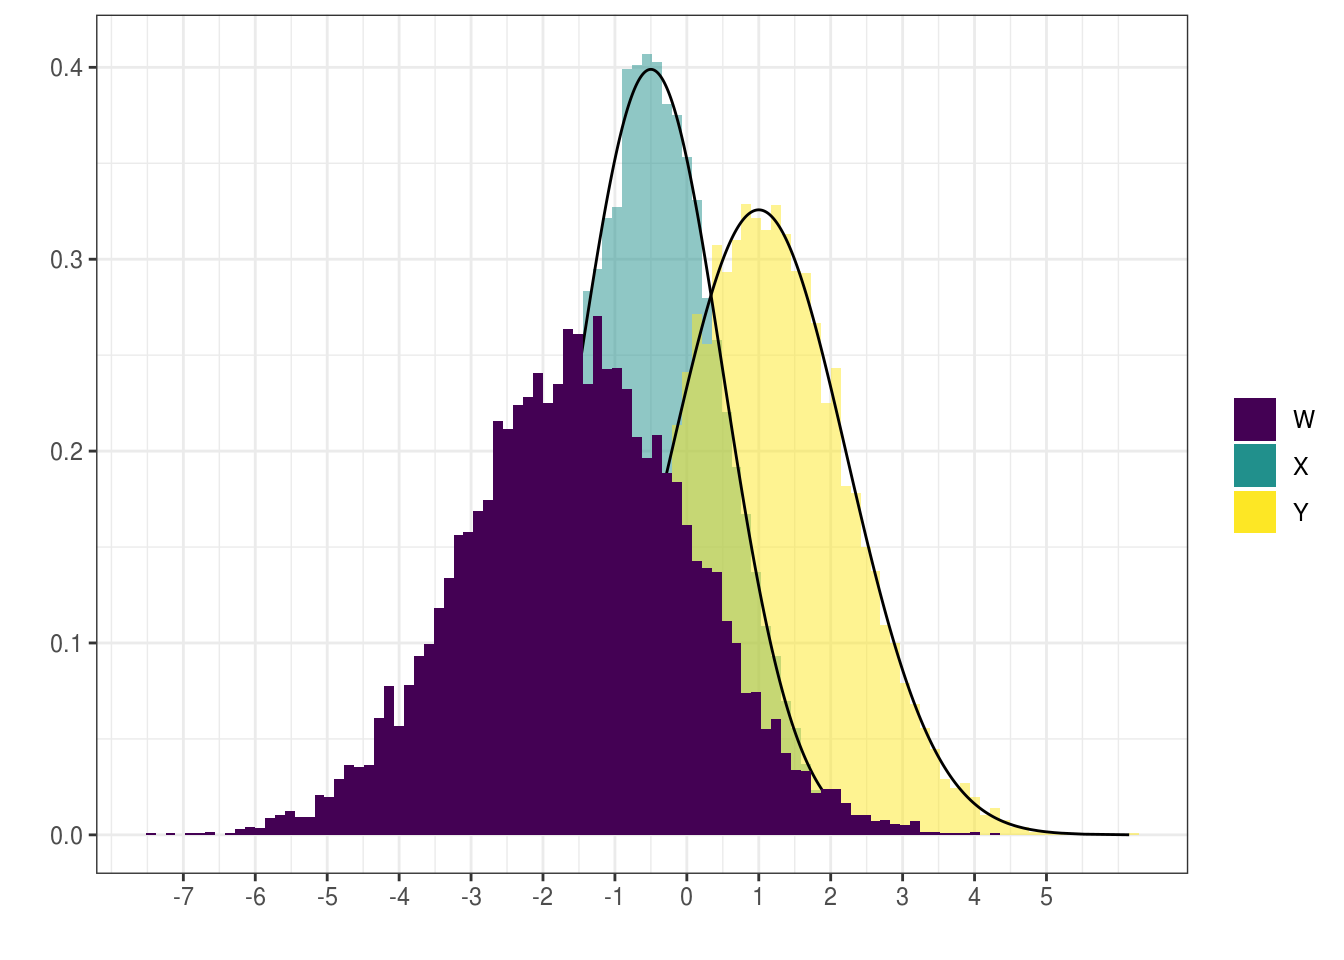
\includegraphics{783_biostats_files/figure-latex/unnamed-chunk-45-1.pdf}

A few things to notice:

\begin{enumerate}
\def\labelenumi{\arabic{enumi}.}
\tightlist
\item
  it most definitely looks like a new normal distribution
\item
  it seems to be centered not far from \(-1.5\)
\item
  it seems to be wider than both of the other curves
\end{enumerate}

So, do these observations match what we would expect?

\begin{enumerate}
\def\labelenumi{\arabic{enumi}.}
\tightlist
\item
  We know that the difference of two normally distributed variables should again be normally distributed
\item
  Our rules tell us that \(E(W) = E(X - Y) = E(X) - E(Y) = -0.5 - 1 = -1.5\), so that also checks out
\item
  The rules stated above also tell us that \(\text{Var}(W) = \text{Var}(X - Y) = \text{Var}(X) + \text{Var}(Y) = 1 + 1.5 = 2.5\), so we do expect the new curve to be wider than both of the old ones.
\end{enumerate}

Finally, we can check that the averages and variances we observe are close to what the theory tells us:

\begin{tabular}{l|r|r|r|r}
\hline
Variable & Average & Observed Variance & Mean & Variance\\
\hline
X & -0.5061716 & 0.9892788 & -0.5 & 1.0\\
\hline
Y & 0.9963078 & 1.5060952 & 1.0 & 1.5\\
\hline
W & -1.5024794 & 2.4628971 & -1.5 & 2.5\\
\hline
\end{tabular}

Again, only small differences between the observed and the expected.

\hypertarget{t-distribution}{%
\subsection{t-distribution}\label{t-distribution}}

The t-distribution is very similar to the normal distribution in that the curve also resembles a bell. Unlike the normal distribution, it only depends on one parameter, which is called the degrees of freedom, or \(df\). We use the notation \(t_{df}\) for a t-distribution with \(df\) degrees of freedom.

The t-distribution is always centered around \(0\), which is also its mean, but the variance depends on the degrees of freedom: if \(X \sim t_{df}\), then \(\text{Var}{X} = \frac{df}{df-2}\) if \(df > 2\), \(\text{Var}{X} = \infty\) if \(1 < df < 2\), and the variance of \(X\) is actually undefined if \(df < 1\).

Below are a few examples of the t-distribution with different degrees of freedom. For comparison, the standard normal is also included. Notice how similar the t-distributions with more than 9 degrees of freedom look, and how they keep getting closer and closer to the standard normal distribution. It can actually be shown that if we had an infinite number of degrees of freedom, then the t-distribution is identical to the standard normal distribution.

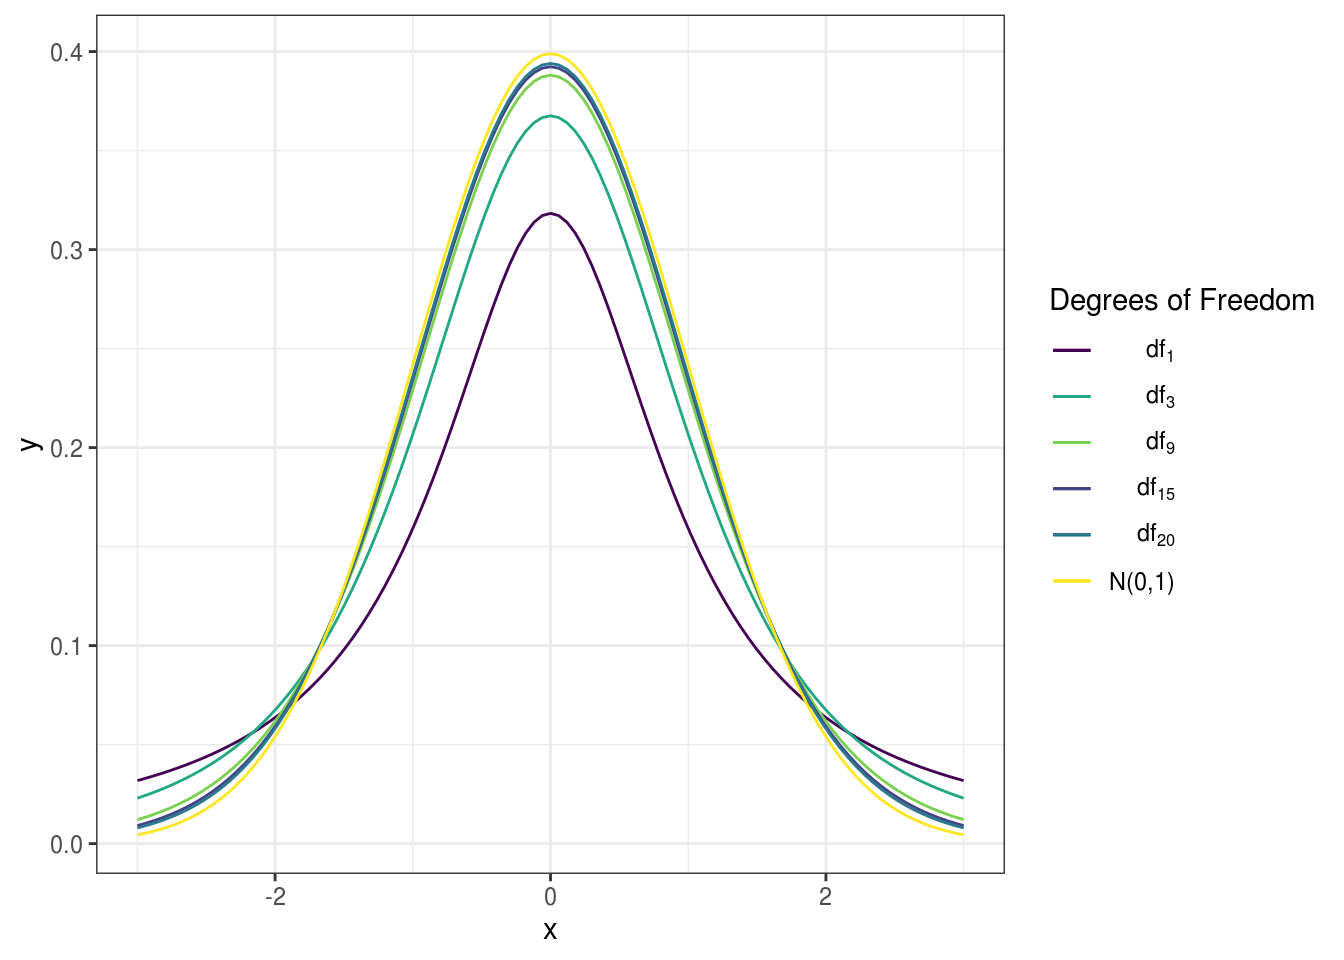
\includegraphics{783_biostats_files/figure-latex/unnamed-chunk-47-1.pdf}

\hypertarget{other-distribution}{%
\subsection{Other Distribution}\label{other-distribution}}

The four distributions above are the ones we'll consider, but there are many, many more out there. Here are a few examples.

\hypertarget{poisson-distribution}{%
\subsubsection{Poisson Distribution}\label{poisson-distribution}}

The Poisson distribution is often used for counting things, such as the number of patients showing up in a clinic during a specified time period. It is a discrete distribution that only returns integer values. It depends on only one parameter which is often referred to as the rate parameter. It is displayed below with a few different values of the rate.

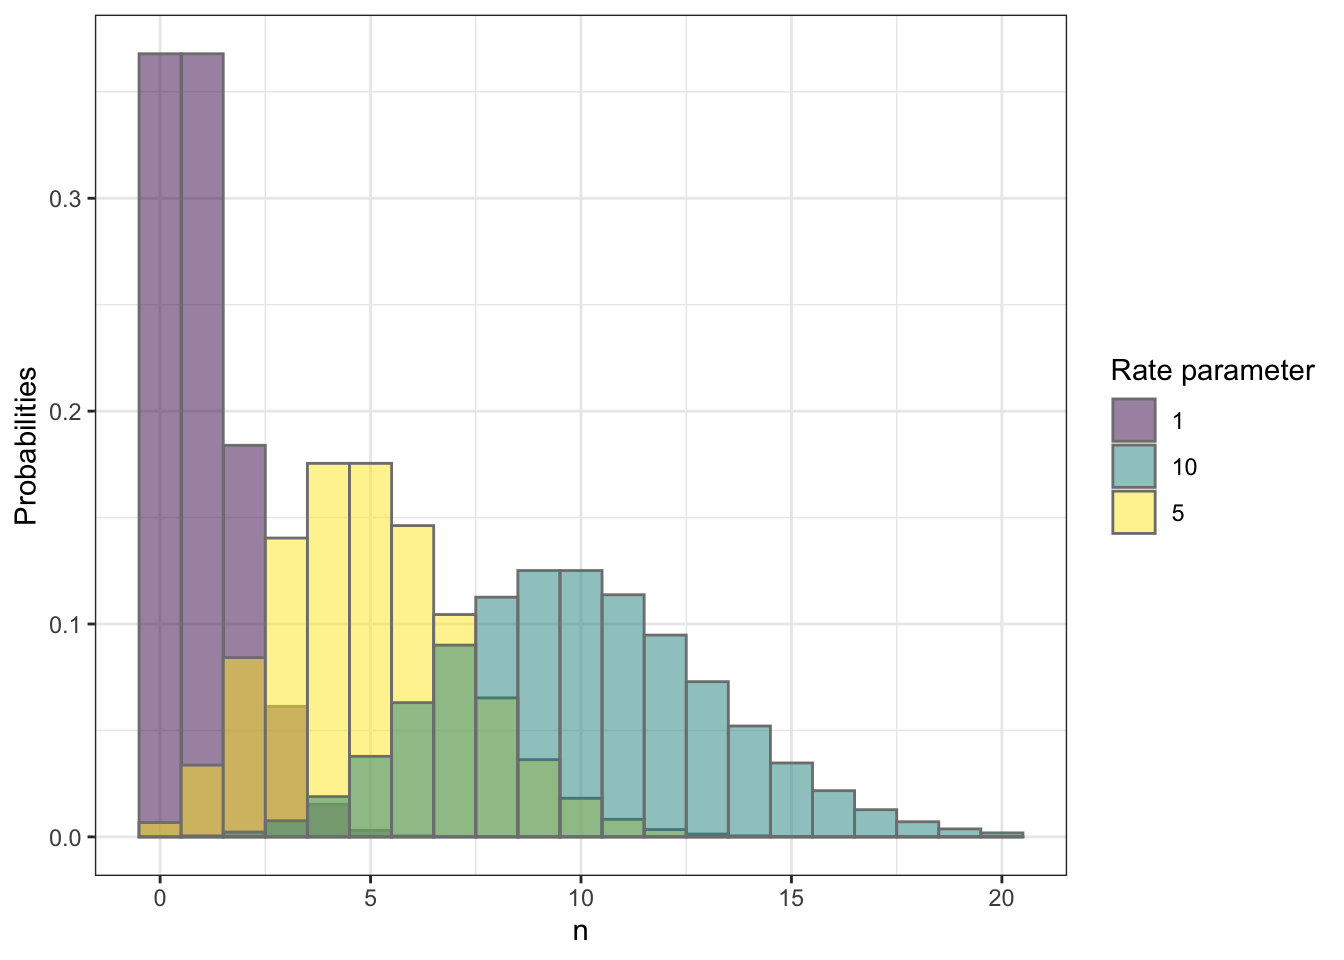
\includegraphics{783_biostats_files/figure-latex/unnamed-chunk-48-1.pdf}

For a Poisson distributed random variable with rate parameter \(\lambda\), \(X \sim \text{Poisson}(\lambda)\), it holds that \(E(X) = \text{Var}(X) = \lambda\).

\hypertarget{exponential-distribution}{%
\subsubsection{Exponential Distribution}\label{exponential-distribution}}

The exponential distribution is often used for wait times. This can be useful if you want to model the wait times in an emergency room, for example. It is a continuous distribution that depends on a single parameter, which is also called the rate parameter.

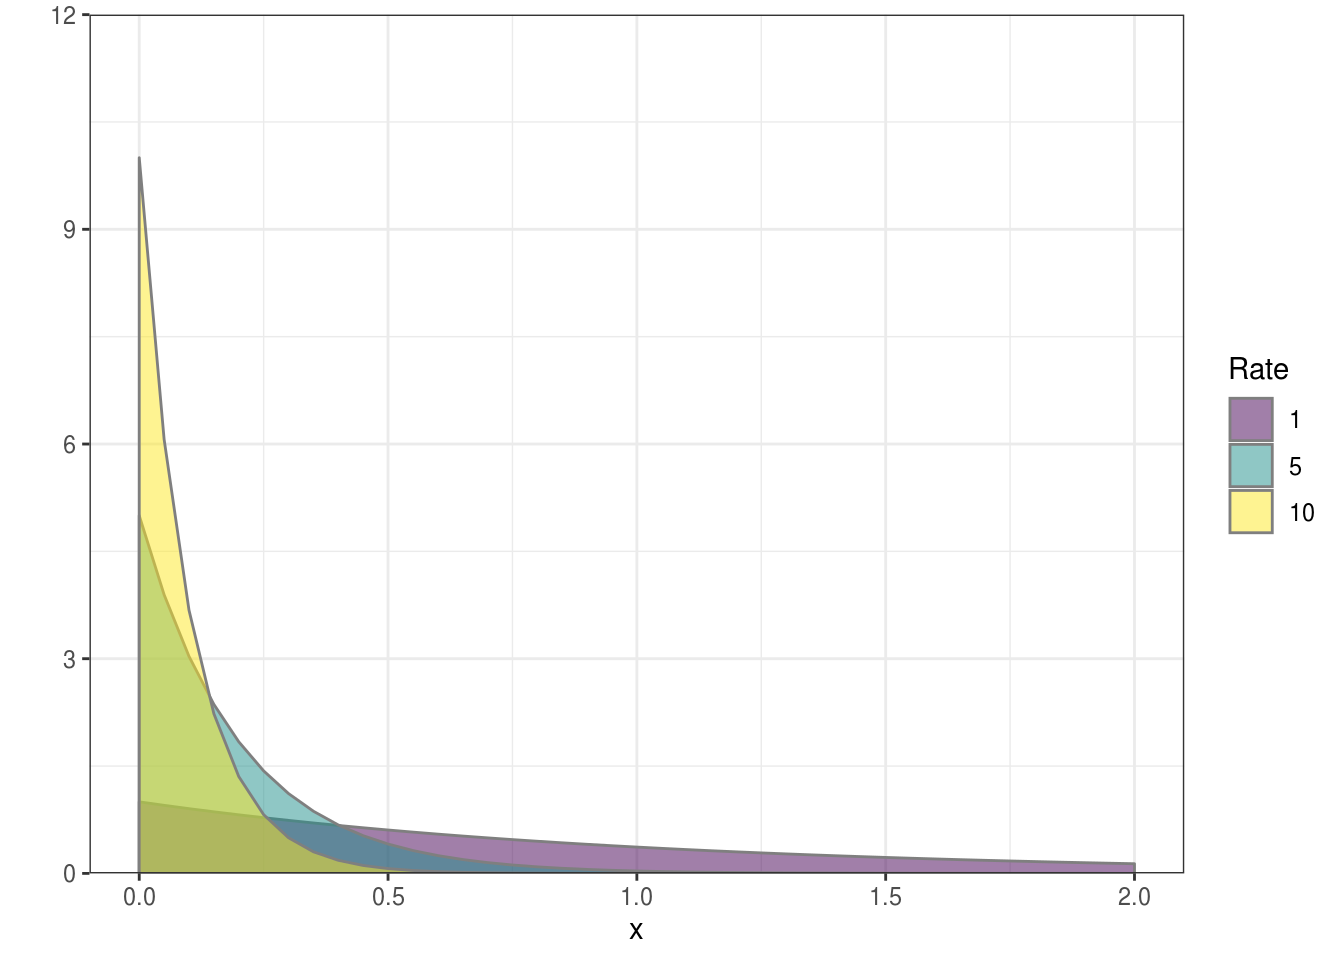
\includegraphics{783_biostats_files/figure-latex/unnamed-chunk-49-1.pdf}

For a random variable that is exponentially distributed with rate parameter \(\lambda\), \(X \sim \text{Exp}(\lambda)\), it holds that \(E(X) = \frac{1}{\lambda}\), and \(\text{Var}(X) = \frac{1}{\lambda^2}\).

\hypertarget{estimators-and-their-distributions}{%
\chapter{Estimators and their distributions}\label{estimators-and-their-distributions}}

In \protect\hyperlink{discrete}{Part I}, we discussed how we can describe and summarize collected data. Different research questions lead you to collect different types of data, and depending on the type of data, there are different ways to present it.

So far in this part, we've talked about these super abstract concepts, such as \protect\hyperlink{what-is-probability}{probabilities}, \protect\hyperlink{random-variables}{random variables} and \protect\hyperlink{a-few-important-distributions}{distributions} that at first seem to have nothing to do with the real world. So why even bother?!

In this section, we will see how random variables and distributions can help us answer questions about the data we collect in the real world. With a few assumptions we will be able to talk about probabilities of real world events, and later on we will use these probabilities to answer questions such as ``is it likely that the mean heights of adult men and women in the US are the same?''

\hypertarget{what-is-an-estimator}{%
\section{What is an Estimator?}\label{what-is-an-estimator}}

Recall the setup: on one hand, we have a population that we are interested in. In this population, there's some feature that we would like to learn more about. This could be either a continuous measurement (such as height, blood pressure, glucose level, etc), or discrete (marital status, disease status, etc). If we could go out and simply inspect every individual in this population, we could learn the truth. We could find out exactly what proportion of the population have a certain disease, what is the mean glucose level among non-diabetics, and so on. Unfortunately, this is not feasible.

What we do instead is we get a sample of individuals from the population. We do this in a way that ensures that this sample is representative of the population, meaning things we might observe in the sample are close to what we would observe in the population, if we had the chance.

After collecting a representative sample, we think for a second about what \emph{parameter} of the population is of interest to us, and then we pick ``something'' we can actually calculate based on our sample that is close to the parameter of interest. This ``something'' is what we call the \emph{estimator} -- it is our best guess of what the parameter is based on a sample. More often than not, the estimator we will use is very natural.

An important thing to realize here is that \textbf{an estimator is a random variable}. The specific value of it depends on the sample we get, which by nature is random. Therefore, repeating the experiment leads to a different value of the estimator. The hope is that the estimator doesn't vary too much when repeating the experiment, and that the estimator is actually close to the true value of the population parameter.

Since an estimator is a random variable, we can talk about the distribution of an estimator. This plays a crucial role when creating confidence intervals and testing hypotheses, as we will see later on in the course. To find the distribution of an estimator, one can take two routes:

\begin{enumerate}
\def\labelenumi{\arabic{enumi}.}
\tightlist
\item
  perform the experiment over and over and over and over again, each time calculating the observed value of the estimator, then drawing a histogram, which in the end will give you the distribution of the estimator,
\item
  make some assumptions, do some math.
\end{enumerate}

The first strategy, as stated here, is not super useful -- we can't possibly afford to repeat a single experiment enough times to get enough observed values of the estimator to actually draw a histogram that provides any insight. However, we can do this for made up data, or using a big data set as a population. As a bonus, this strategy can actually be tweaked a tiny bit to make it not only useful in practice, but super powerful.

The second strategy, although it sounds scary and really hard, turns out to be very useful in a large handful of settings using nothing more complicated than the rules we derived in section \ref{prop-of-RVs} and THE coolest theorem we will see in this class, namely the Central Limit Theorem.

The rest of this section will proceed as follows: first, we'll see a few examples of common estimators. Then, we will explore the distributions of those estimators through simulations where we'll use the SHOW data set as our population. Then we will take a look at the Central Limit Theorem, and how we can apply that to back up the distributions we found for different estimators through simulations.

Before we get started, a small comment on notation. Going forward, we will use greek letters to denote the true parameters (i.e.~the values in the population that we will never really know), and latin letters to denote estimators, and observed values of estimators.

\hypertarget{common-estimators}{%
\section{Common Estimators}\label{common-estimators}}

Some things we are often interested in and their estimators:

\begin{longtable}[]{@{}ccc@{}}
\toprule
\begin{minipage}[b]{0.35\columnwidth}\centering
Parameter of Interest (most commonly used symbol)\strut
\end{minipage} & \begin{minipage}[b]{0.21\columnwidth}\centering
Estimator Name\strut
\end{minipage} & \begin{minipage}[b]{0.35\columnwidth}\centering
Notation and Formula\strut
\end{minipage}\tabularnewline
\midrule
\endhead
\begin{minipage}[t]{0.35\columnwidth}\centering
Mean of a feature (\(\mu\))\strut
\end{minipage} & \begin{minipage}[t]{0.21\columnwidth}\centering
Sample average\strut
\end{minipage} & \begin{minipage}[t]{0.35\columnwidth}\centering
\(\bar{X} = \frac{1}{n} \sum_{i=1}^n X_i\)\strut
\end{minipage}\tabularnewline
\begin{minipage}[t]{0.35\columnwidth}\centering
Variance of a feature (\(\sigma^2\))\strut
\end{minipage} & \begin{minipage}[t]{0.21\columnwidth}\centering
Sample variance\strut
\end{minipage} & \begin{minipage}[t]{0.35\columnwidth}\centering
\(S^2 = \frac{1}{n-1} \sum_{i=1}^n (X_i - \bar{X})^2\)\strut
\end{minipage}\tabularnewline
\begin{minipage}[t]{0.35\columnwidth}\centering
Standard deviation (\(\sigma\))\strut
\end{minipage} & \begin{minipage}[t]{0.21\columnwidth}\centering
Sample standard deviation\strut
\end{minipage} & \begin{minipage}[t]{0.35\columnwidth}\centering
\(S = \sqrt{\frac{1}{n-1} \sum_{i=1}^n (X_i - \bar{X})^2}\)\strut
\end{minipage}\tabularnewline
\begin{minipage}[t]{0.35\columnwidth}\centering
Probability of random individual having a disease (\(\pi\))\strut
\end{minipage} & \begin{minipage}[t]{0.21\columnwidth}\centering
Proportion in sample with disease\strut
\end{minipage} & \begin{minipage}[t]{0.35\columnwidth}\centering
\(P = \frac{1}{n}\sum_{i=1}^n X_i\)\strut
\end{minipage}\tabularnewline
\begin{minipage}[t]{0.35\columnwidth}\centering
Proportion of individuals with disease (\(\pi\))\strut
\end{minipage} & \begin{minipage}[t]{0.21\columnwidth}\centering
Proportion in sample with disease\strut
\end{minipage} & \begin{minipage}[t]{0.35\columnwidth}\centering
\(P = \frac{1}{n}\sum_{i=1}^n X_i\)\strut
\end{minipage}\tabularnewline
\bottomrule
\end{longtable}

As you can see in the table above, most of the estimators we will consider here are pretty much what you would expect. If you are interested in the mean of the population, you look at the average (or \emph{mean}) of the sample. Interested in the proportion of individuals with a disease in the population? Consider the proportion with that disease in your sample.

\hypertarget{examples-5}{%
\subsection{Examples}\label{examples-5}}

In the following examples, we'll play a game of pretend: pretend that the SHOW cohort is the \emph{entire} population, and that we would like to estimate different things in this population.

\hypertarget{estimating-mean-height}{%
\subsubsection*{Estimating Mean Height}\label{estimating-mean-height}}
\addcontentsline{toc}{subsubsection}{Estimating Mean Height}

Say I ask you to estimate the mean height of the subjects in the SHOW population. I won't show you the entire population, but I will let you pick a simple random sample of size 20 from the population. You do just that, and you get the following sample.

\hypertarget{htmlwidget-f60428f63ee038fbf512}{}

Based on this sample, what would be your best guess as to what the true mean height of the entire population is? Since the sample is a simple random sample, you would probably go with the average: 168.5925. But how certain are you that your estimate is a good? What's to say that it's not super far from the true population mean height?

One way to answer this question is by thinking about the distribution of the average of 20 samples. If we can get an idea of what the distribution of this is compared to the true population mean height (which we know in this case, since the SHOW cohort is the entire population), then we can maybe say something about how likely we are to be ``close'' to the population mean. To get a better idea of what the distribution of the sample average is, we can create many, many samples of size 20 from the population, calculate the average height for each of them, and then create a histogram. Since we have the entire population available, we can also calculate the true population mean height, and then see how the distribution of the sample average compares.

So, let us do just that. First of all, the true population mean height is 169.3721876, which is simply the average of ALL subjects in the population. Furthermore, we can consider the distribution of the individual heights:

\begin{figure}
\centering
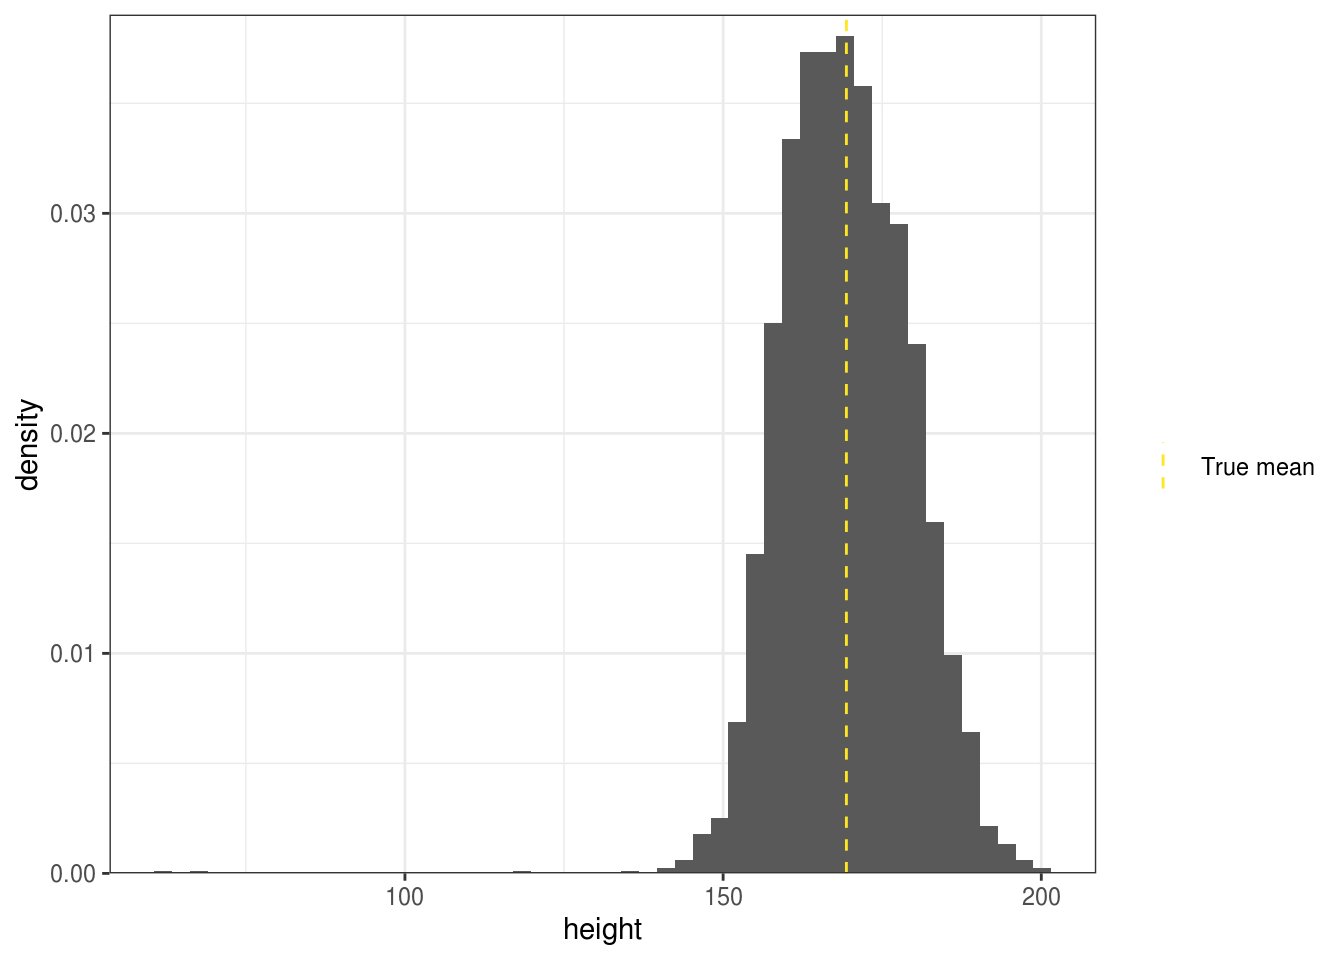
\includegraphics{783_biostats_files/figure-latex/pop-dist-height-1.pdf}
\caption{\label{fig:pop-dist-height}Population distribution of height}
\end{figure}

Now, the first sample we got gave us an average of 168.5925. We sample from the population one more time, and this time end up with this sample:

\hypertarget{htmlwidget-08479c68cbb6859f9bdd}{}

As you can see, in this sample we have different subjects (i.e.~different id's), as we would expect when sampling only 20 subjects out of a total of 2934. From this new sample, we get a sample average of 170.46. As you can see, this is indeed different than the average height of the first sample. Now, we do this over and over and over again, a total of \ensuremath{10^{4}} times. So, in the end, we have \ensuremath{10^{4}} samples, and for each sample, we calculate an average. All of these averages can be used to create a histogram, which gives us a great approximation of the distribution of the sample average (with n = 20):

\begin{figure}
\centering
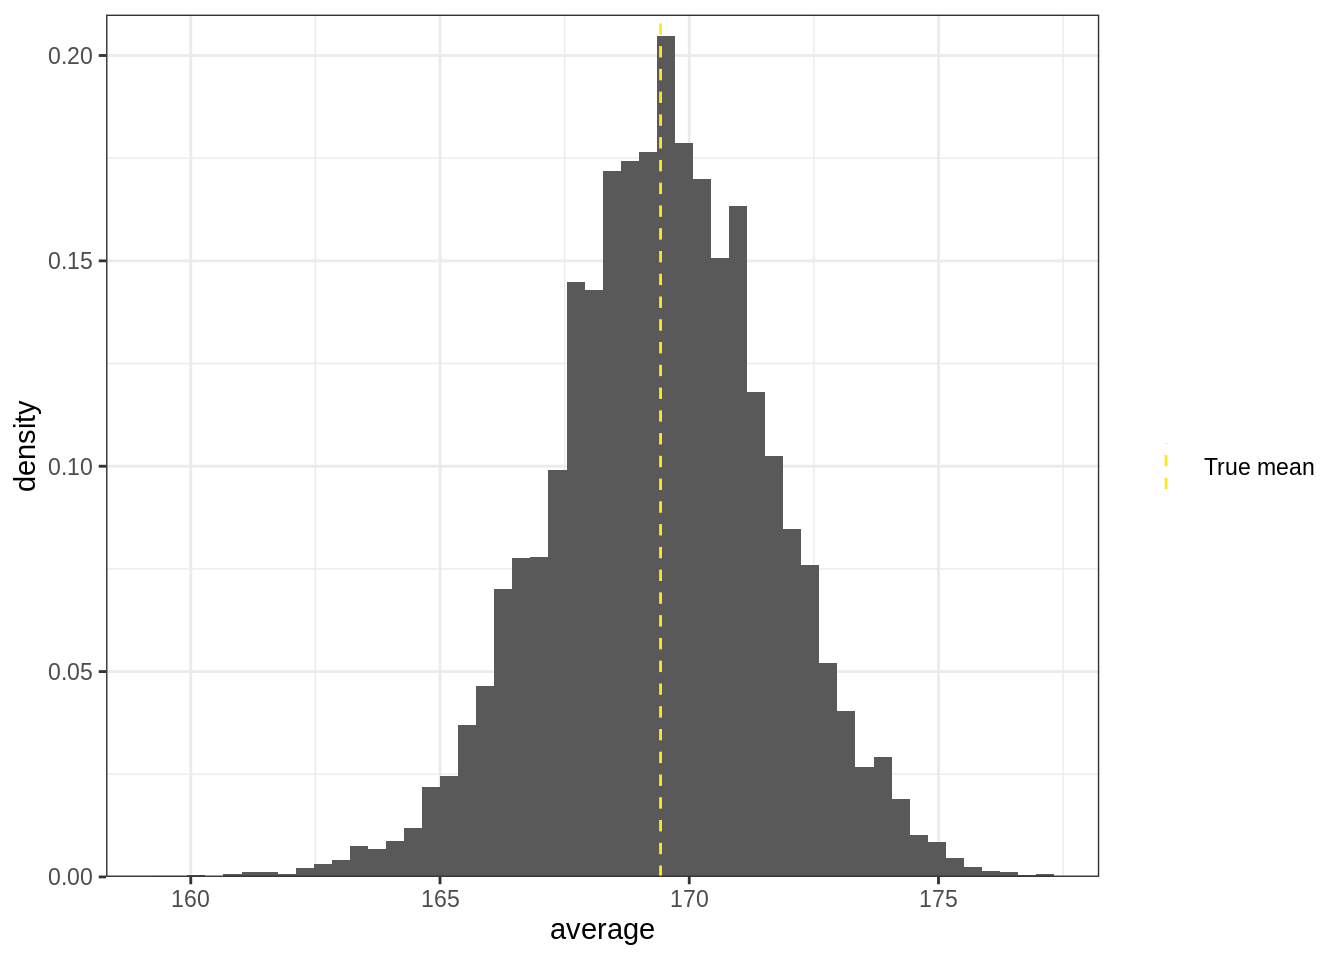
\includegraphics{783_biostats_files/figure-latex/height-averages-histogram-1.pdf}
\caption{\label{fig:height-averages-histogram}Distribution of average heights.}
\end{figure}

A few things to note here:

\begin{enumerate}
\def\labelenumi{\arabic{enumi}.}
\tightlist
\item
  Look how nicely the distribution is centered around the true population mean! This mean that using the sample average as an estimator of the true population mean might not be an entirely bad idea: in general, we are more likely to get an average that is ``close'' to the truth!
\item
  The shape of that distribution looks an awful lot like a normal distribution, don't you think? Coincidence? Maybe. Maybe not\ldots{}
\item
  This histogram is a lot narrower than that of the actual heights. To really see that, the figure below shows both distributions overlayed one another. This tells us that to get a good idea of the true mean population height, it's a much better idea to create a sample of 20 subjects and use their average as your best guess than to simply sample a single individual, and use their height. Probably not surprising. But if you think of the height of a single individual as ``an average of a sample of size 1'', and the true value as ``an anverage of a sample of size \(\infty\)'' (here, \(\infty\) equals the total population), then you might realize a pattern: the small sample size (sample size of 1) is worse than the medium sample size (20), which is worse than the ideal sample size (\(\infty\)). It seems that your guess gets better as you increase the sample size\ldots{} Coincidence? Maybe. Maybe not\ldots{}
\end{enumerate}

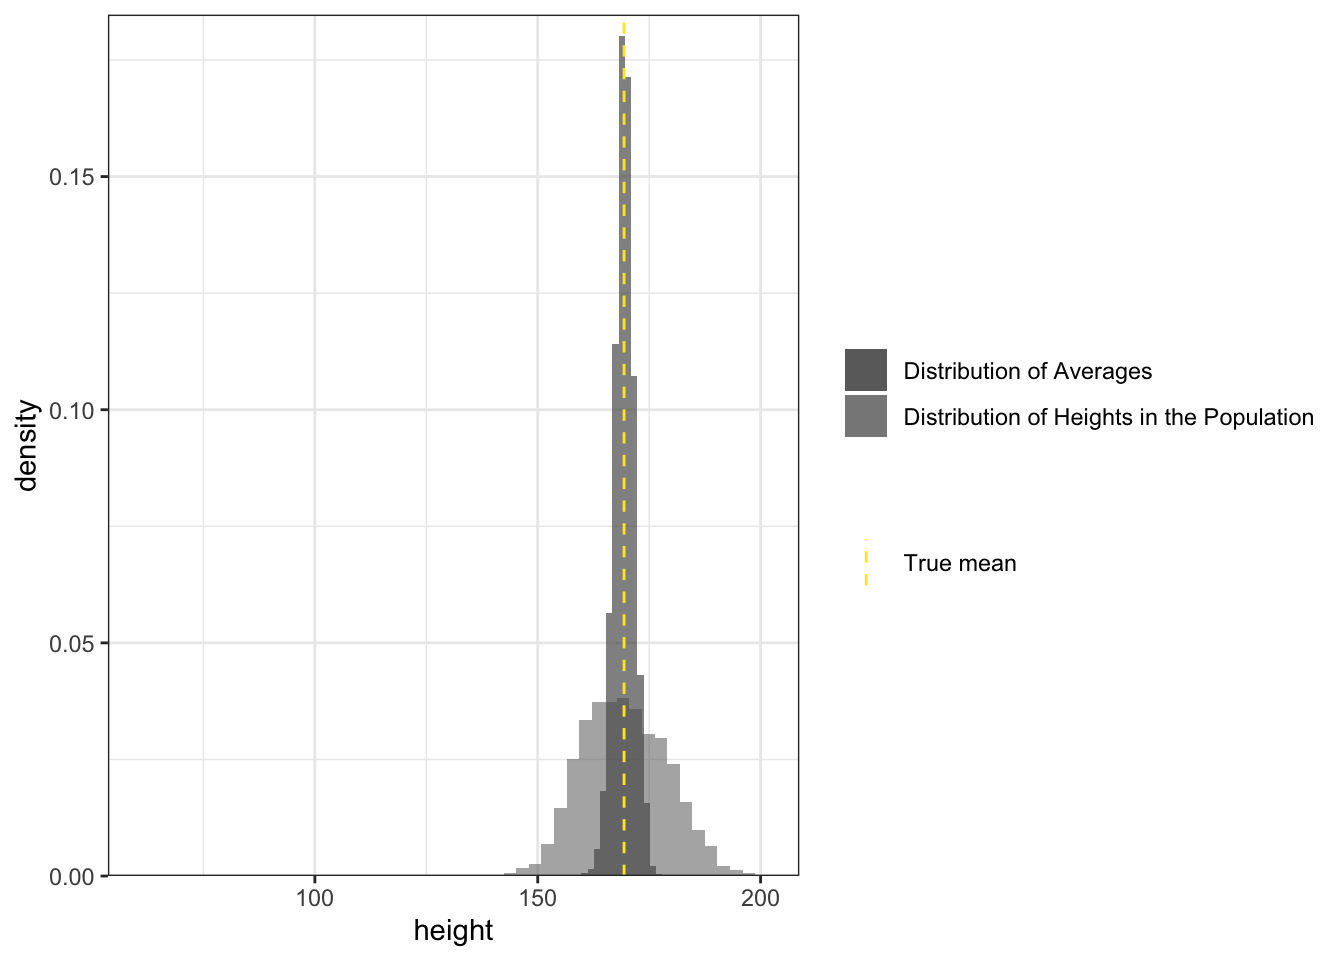
\includegraphics{783_biostats_files/figure-latex/unnamed-chunk-54-1.pdf}

\hypertarget{estimating-mean-depression-score}{%
\subsubsection*{Estimating Mean Depression Score}\label{estimating-mean-depression-score}}
\addcontentsline{toc}{subsubsection}{Estimating Mean Depression Score}

Of the three bullet points above, the one that to me is the most surprising is the second one. Points 1 and 3 seem pretty intuitive: the former says that the average is a good substitute for the mean, the third that bigger sample size is better. Not exactly mind blowing. The second one, however, is more intriguing, although in the previous case, maybe not so much. After all, the distribution of the population (i.e.~the distribution of all heights, shown in \ref{fig:pop-dist-height}) looks a whole lot like a normal distribution in the first place.

Let's take a look at what happens if we consider something that is nothing like a normal distribution. Let's say we would like to estimate the mean depression score in the population. The procedure is the same as before. Take a sample, calculate the average, repeat a bunch of times to get a good approximation of the distribution.

Here, we take samples of 50. The first sample came out to consist of the following subjects:

\hypertarget{htmlwidget-d7c813a12909b2ec0869}{}

The average depression score in this sample is 3.1. Rinse and repeat 10000 times.

Before we take a look at the distribution of all the averages, let's consider the distribution of the depression scores in the entire population.

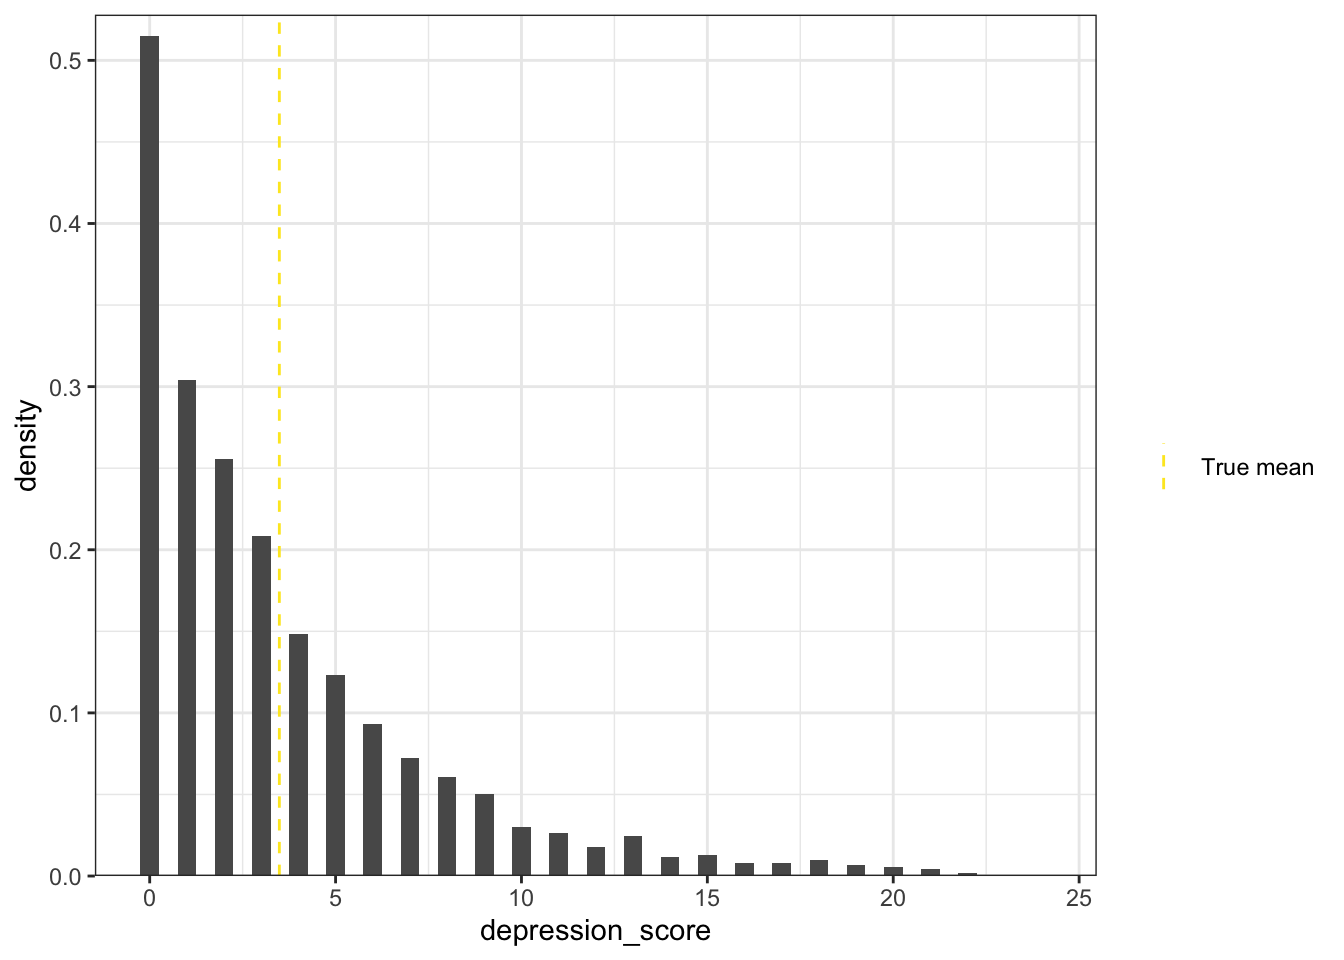
\includegraphics{783_biostats_files/figure-latex/unnamed-chunk-57-1.pdf}

This is nothing like a normal distribution at all! By nature, this distribution is discrete (each observation is a score from 0 to 25), and it is not symmetrical around the mean. But take a look at what the distribution of the averages looks like:

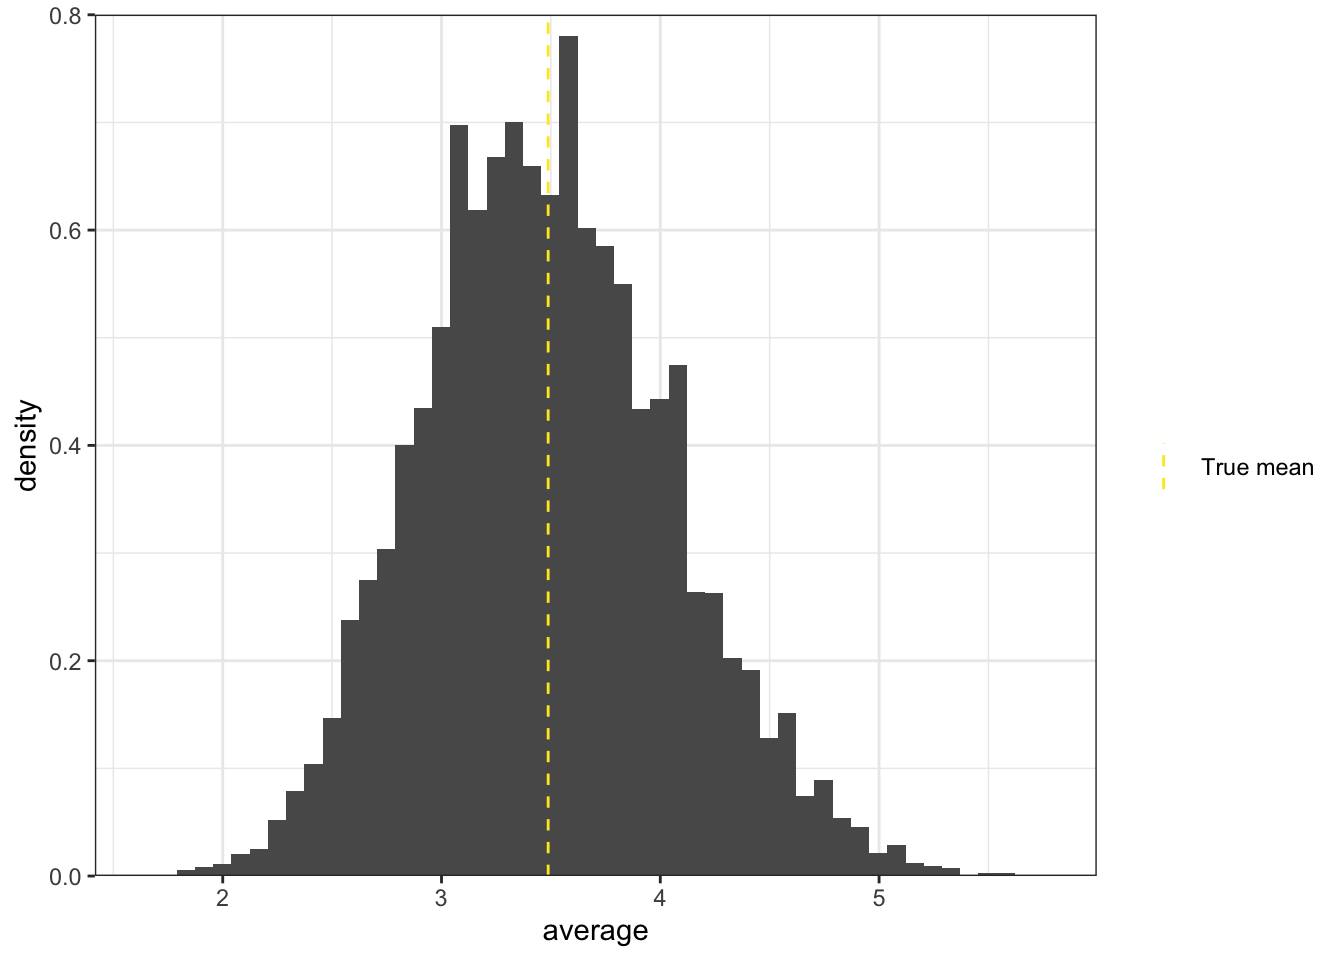
\includegraphics{783_biostats_files/figure-latex/unnamed-chunk-58-1.pdf}

\begin{enumerate}
\def\labelenumi{\arabic{enumi}.}
\tightlist
\item
  Pretty symmetrical.
\item
  Centered around the true mean.
\item
  Looks pretty bell-shaped to me.
\end{enumerate}

In other words, saying that this distribution is (at least approximately) normal does not seem like a stretch to me!

\hypertarget{estimating-proportion-of-men}{%
\subsubsection*{Estimating Proportion of Men}\label{estimating-proportion-of-men}}
\addcontentsline{toc}{subsubsection}{Estimating Proportion of Men}

Next, let's consider what to do if we were instead interested in the proportion of the population that are men From a simple random sample of size 20, I would argue that the best guess for the true proportion of women in the population is the sample proportion: the number of women out of the total number of individuals in the sample. Seems intuitively sound. Let's got through the same motion that we did with the means above: sample a bunch of times from the population, each time calculate the sample proportion, then consider the histogram.

First, the true distribution of the gender variable in the data. Here, \(0\) is stand-in for women, \(1\) stand-in for men.

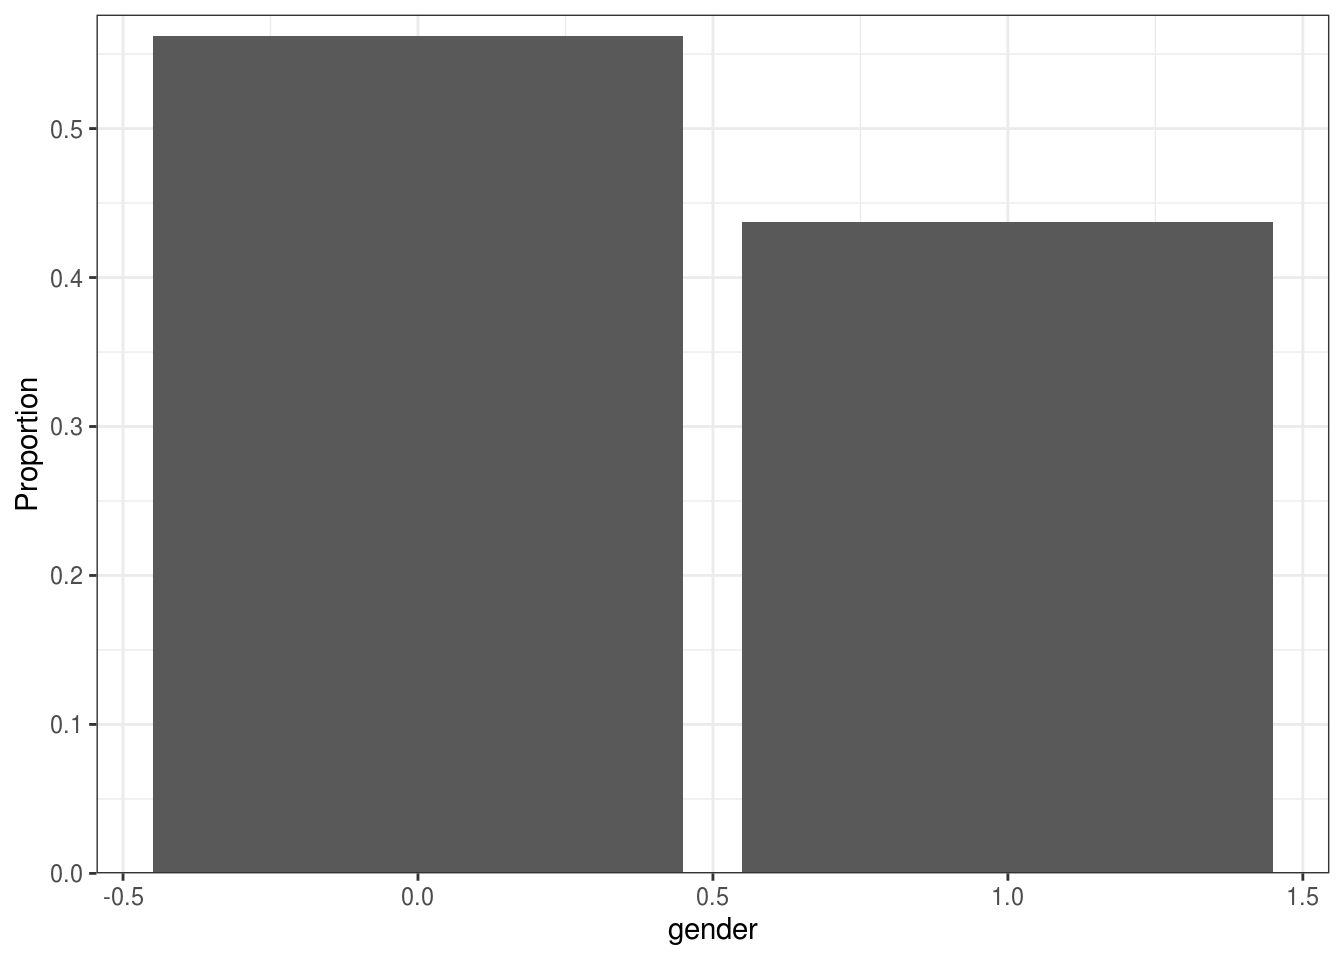
\includegraphics{783_biostats_files/figure-latex/unnamed-chunk-59-1.pdf}

We see that the true proportion of the population that are men is 0.44.

Next, let's take a look at the distribution of sample proportions.

\includegraphics{figures/gender_props_histogram.png}

Again, it looks pretty normal! How can that be?!

The truth is, as we will see later on, a proportion is really not that different from an average. Since the gender variable is \(1\) for all men, and \(0\) for all women, then the proportion of men is really calculated as \(\frac{1}{n}\sum_{i=1}^n g_i\), where \(g_i\) is \(1\) if the \(i\)'th subject is male, and \(0\) otherwise. So, the proportion is really an average, and therefore it might not be that big of a surprise that the distribution of the sample proportions is approximately normal.

\hypertarget{estimating-relative-risk}{%
\subsubsection*{Estimating Relative Risk}\label{estimating-relative-risk}}
\addcontentsline{toc}{subsubsection}{Estimating Relative Risk}

So far, we've seen three examples, but they've really all dealt with one estimator: namely the average. (As mentioned, even the proportion can be considered an average.) Let's turn to something that does NOT turn out to be normally distributed.

Say we are interested in the relative risk of being severely depressed between men and women. It seems reasonable that a good estimate of the relative risk in the population is simply the relative risk in the sample we get. Let's take a look.

We create simple random samples of size 75. The first sample consists of the following individuals:

\hypertarget{htmlwidget-b9150501cb8ba77e69a3}{}

To find the relative risk, we create the 2 by 2 contingency table for \texttt{gender} and \texttt{depression\_severity\_binary}:

\begin{longtable}[]{@{}cccc@{}}
\toprule
\begin{minipage}[b]{0.36\columnwidth}\centering
depression\_severity\_binary\strut
\end{minipage} & \begin{minipage}[b]{0.11\columnwidth}\centering
Female\strut
\end{minipage} & \begin{minipage}[b]{0.09\columnwidth}\centering
Male\strut
\end{minipage} & \begin{minipage}[b]{0.10\columnwidth}\centering
Total\strut
\end{minipage}\tabularnewline
\midrule
\endhead
\begin{minipage}[t]{0.36\columnwidth}\centering
0\strut
\end{minipage} & \begin{minipage}[t]{0.11\columnwidth}\centering
24\strut
\end{minipage} & \begin{minipage}[t]{0.09\columnwidth}\centering
31\strut
\end{minipage} & \begin{minipage}[t]{0.10\columnwidth}\centering
55\strut
\end{minipage}\tabularnewline
\begin{minipage}[t]{0.36\columnwidth}\centering
1\strut
\end{minipage} & \begin{minipage}[t]{0.11\columnwidth}\centering
12\strut
\end{minipage} & \begin{minipage}[t]{0.09\columnwidth}\centering
8\strut
\end{minipage} & \begin{minipage}[t]{0.10\columnwidth}\centering
20\strut
\end{minipage}\tabularnewline
\begin{minipage}[t]{0.36\columnwidth}\centering
Total\strut
\end{minipage} & \begin{minipage}[t]{0.11\columnwidth}\centering
36\strut
\end{minipage} & \begin{minipage}[t]{0.09\columnwidth}\centering
39\strut
\end{minipage} & \begin{minipage}[t]{0.10\columnwidth}\centering
75\strut
\end{minipage}\tabularnewline
\bottomrule
\end{longtable}

The relative risk is then calculated as

\begin{align*}
  \frac{\text{proportion of males with severe depression}}{\text{proportion of women with severe depression}} &= \frac{17/29}{11/21} \\ & \approx 0.62.
\end{align*}

As before, we repeat this many, many times, and plot the results as a histogram, which gives us an approximate distribution of the relative risk in a sample of 75 subjects.

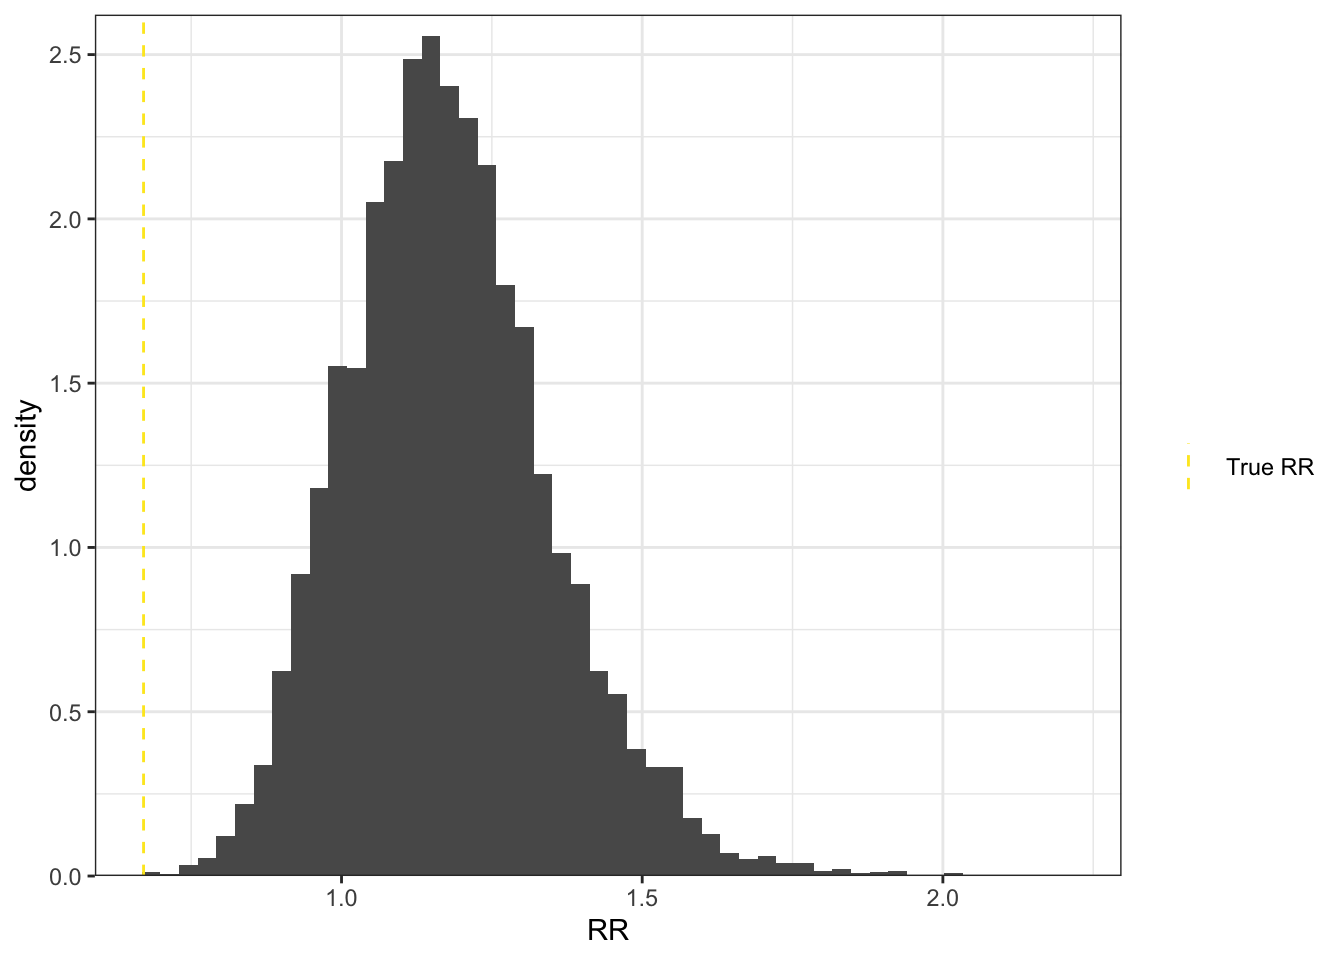
\includegraphics{783_biostats_files/figure-latex/unnamed-chunk-64-1.pdf}

The first thing we probably notice is that this is not a normal distribution. It is not symmetrical, and therefore also not bell-shaped. However, it is very nicely distributed around the true population relative risk.

So, for the first time we end up with something that is not normally distributed. This is not in and of itself a huge problem, but it does make life a bit harder later on. In this particular case, however, there is a very simple fix: instead of considering the relative risk, consider \(\log(RR)\), the log transformed relative risk:

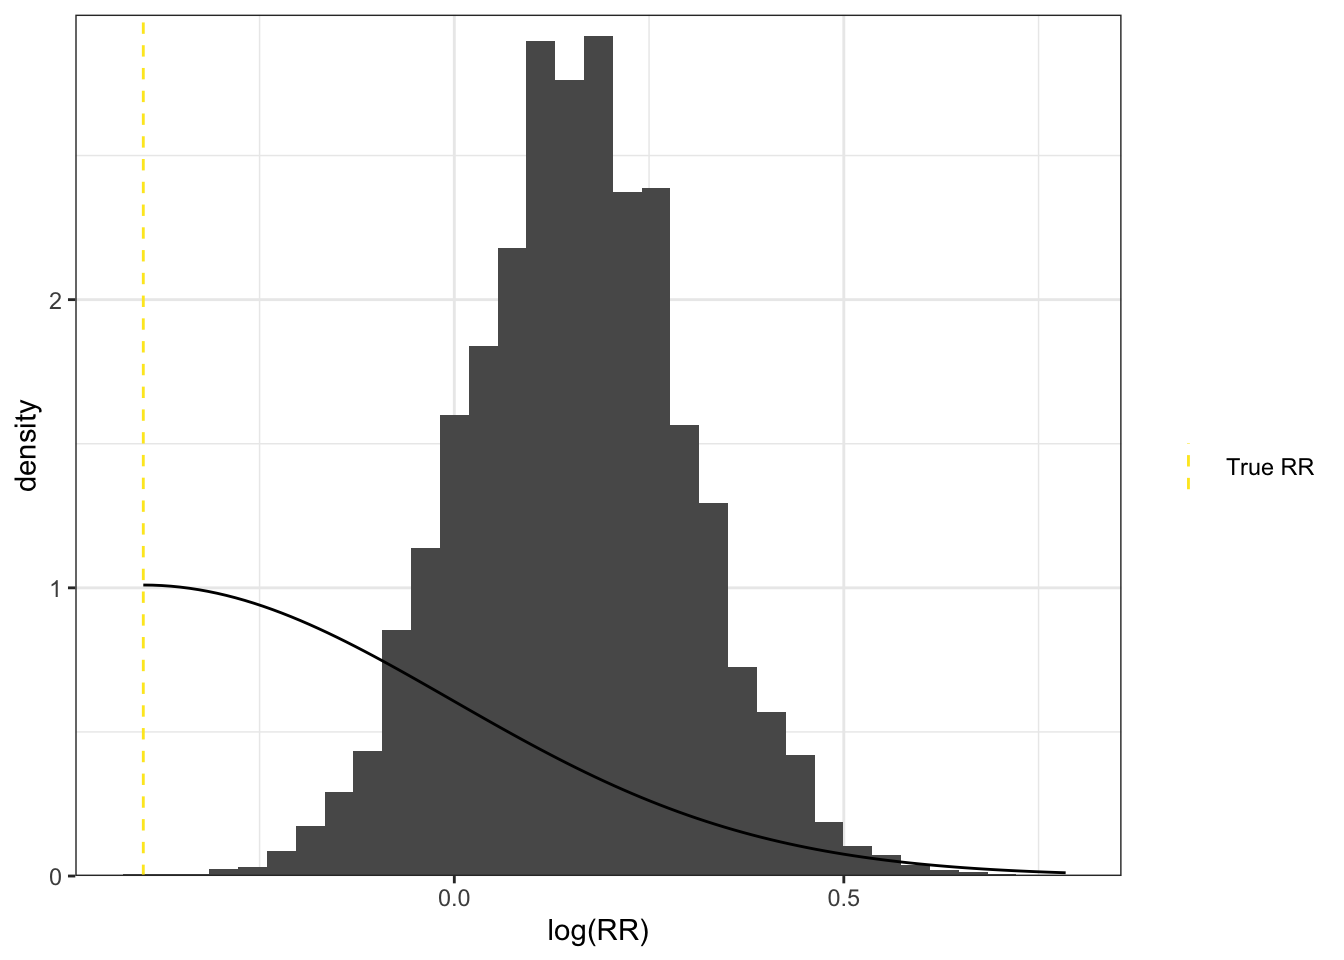
\includegraphics{783_biostats_files/figure-latex/unnamed-chunk-65-1.pdf}

Looks pretty normal, huh? We will (ab)use this fact later on.

\hypertarget{estimating-odds-ratios}{%
\subsubsection*{Estimating Odds Ratios}\label{estimating-odds-ratios}}
\addcontentsline{toc}{subsubsection}{Estimating Odds Ratios}

Here we repeat the previous section, but estimating the odds ratio instead of the relative risk. Same comments apply.

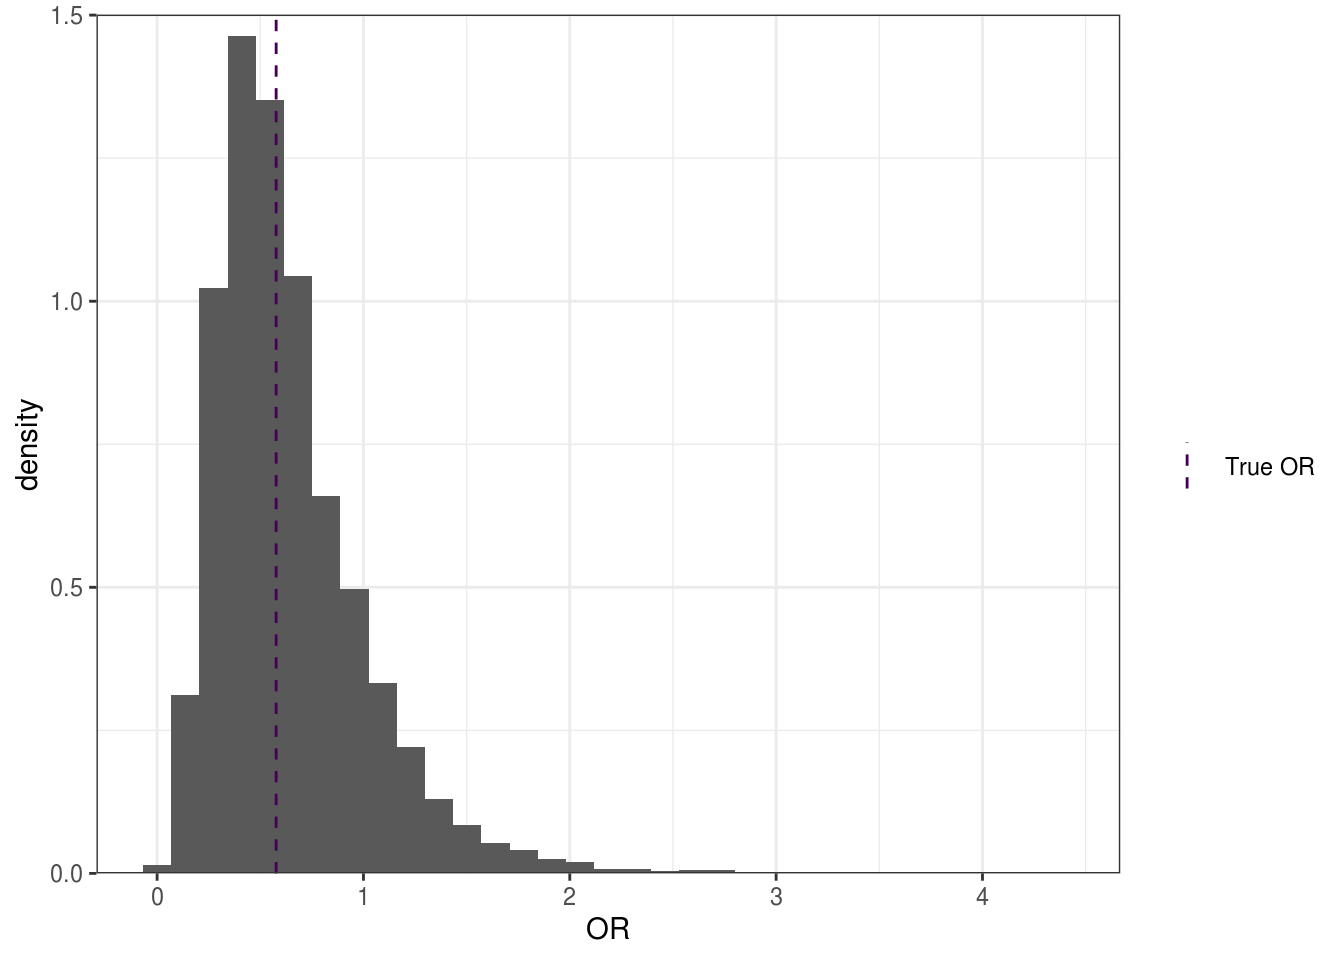
\includegraphics{783_biostats_files/figure-latex/unnamed-chunk-66-1.pdf}

Definitely not normal. But if we log transform\ldots{}

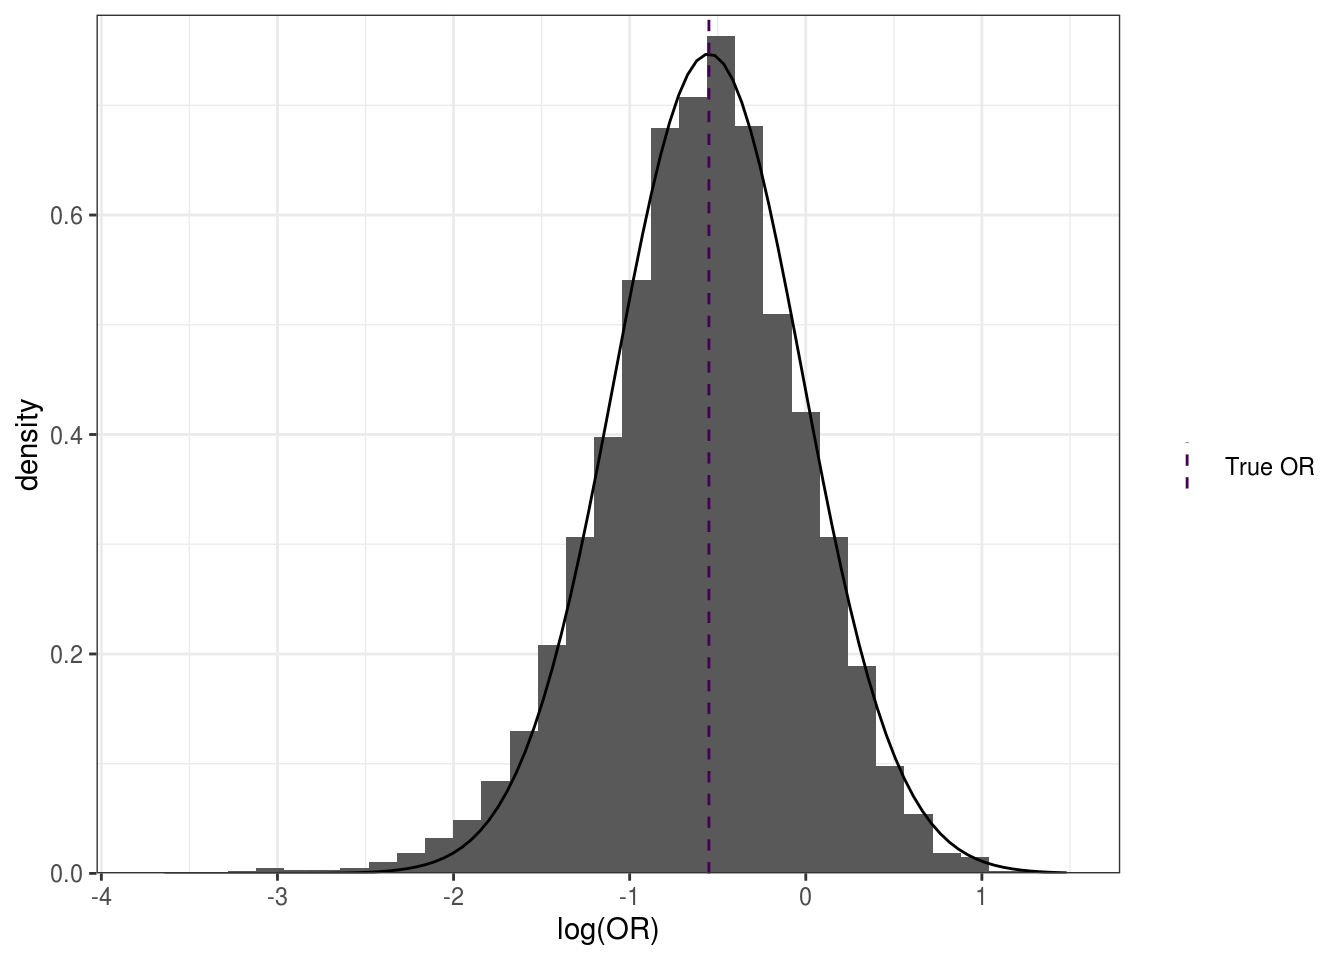
\includegraphics{783_biostats_files/figure-latex/unnamed-chunk-67-1.pdf}

\hypertarget{deriving-distributions-in-practice}{%
\section{Deriving Distributions in Practice}\label{deriving-distributions-in-practice}}

In the previous section, we considered quite a few examples of estimators, and saw how we can get a very good idea of exactly what the distribution of an estimator is \emph{when we have the entire population at our disposal}. This is basically never the case. Even if we had a way of getting in touch with the entire popoulation, and create thousands and thousands of simple random samples, it is very unlikely we would have the time and funds to do so. So, in practice, we have to do something else to find the distribution of the estimator we're interested in. Here, we will discuss how to do so using what I think is \emph{the} coolest result we will encounter in this class, namely the \emph{Central Limit Theorem}.

\hypertarget{CLT}{%
\subsection{The Central Limit Theorem}\label{CLT}}

Let's jump right to it, and state the Central Limit Theorem:

\BeginKnitrBlock{theorem}[The Central Limit Theorem]
\protect\hypertarget{thm:theCLT}{}{\label{thm:theCLT} \iffalse (The Central Limit Theorem) \fi{} }Let \(X_1, X_2, ..., X_n\) be a simple random sample from a population with mean \(\mu\) and variance \(\sigma^2\) (i.e.~\(E(X_i) = \mu\) and \(\text{Var}(X_i) = \sigma^2\) for all \(i\)). Then, as long as \(n\) is large enough, the \emph{average} \(\bar{X} = \frac{1}{n} \sum_{i=1}^n X_i\) is approximately \(N(\mu, \sigma^2 / n)\).
\EndKnitrBlock{theorem}

So what's so special about this? It's a rather simple setup: if you have a simple random sample of size ``big enough'', then the average is going to be normally distributed with mean \(\mu\) and variance \(\sigma^2/n\). But think about this for a second: there are no assumptions on where you start, and yet we get that we end up with something that is normally distributed!

Let's revisit the examples from above.

\hypertarget{estimating-mean-height-1}{%
\subsubsection*{Estimating Mean Height}\label{estimating-mean-height-1}}
\addcontentsline{toc}{subsubsection}{Estimating Mean Height}

We saw previously that if we create 10000 samples from the SHOW population, calculate the average height of each sample, and then create a histogram of all these averages, it would result in something like figure \ref{fig:height-averages-histogram}. Just by looking at this, we observed it looked a lot like a normal distribution. Now, with the CLT at hand, we can actually find the exact normal distribution that it follows.

Since we know the true mean and variance (the mean and variance of the entire population), we can find the specific normal distribution that the CLT tells us this distribution should be much like.

From the SHOW population, we find that the mean height is \(\mu = 169.37\), and the variance is \(\sigma^2 = 98.54\). So, since the sample size here was \(n = 20\), the CLT tells us that \(\bar{X} \sim N(169.37, 98.54/20)\). How does this fit the histogram? The black line below is that exact normal distribution. Fits pretty well, if you ask me.

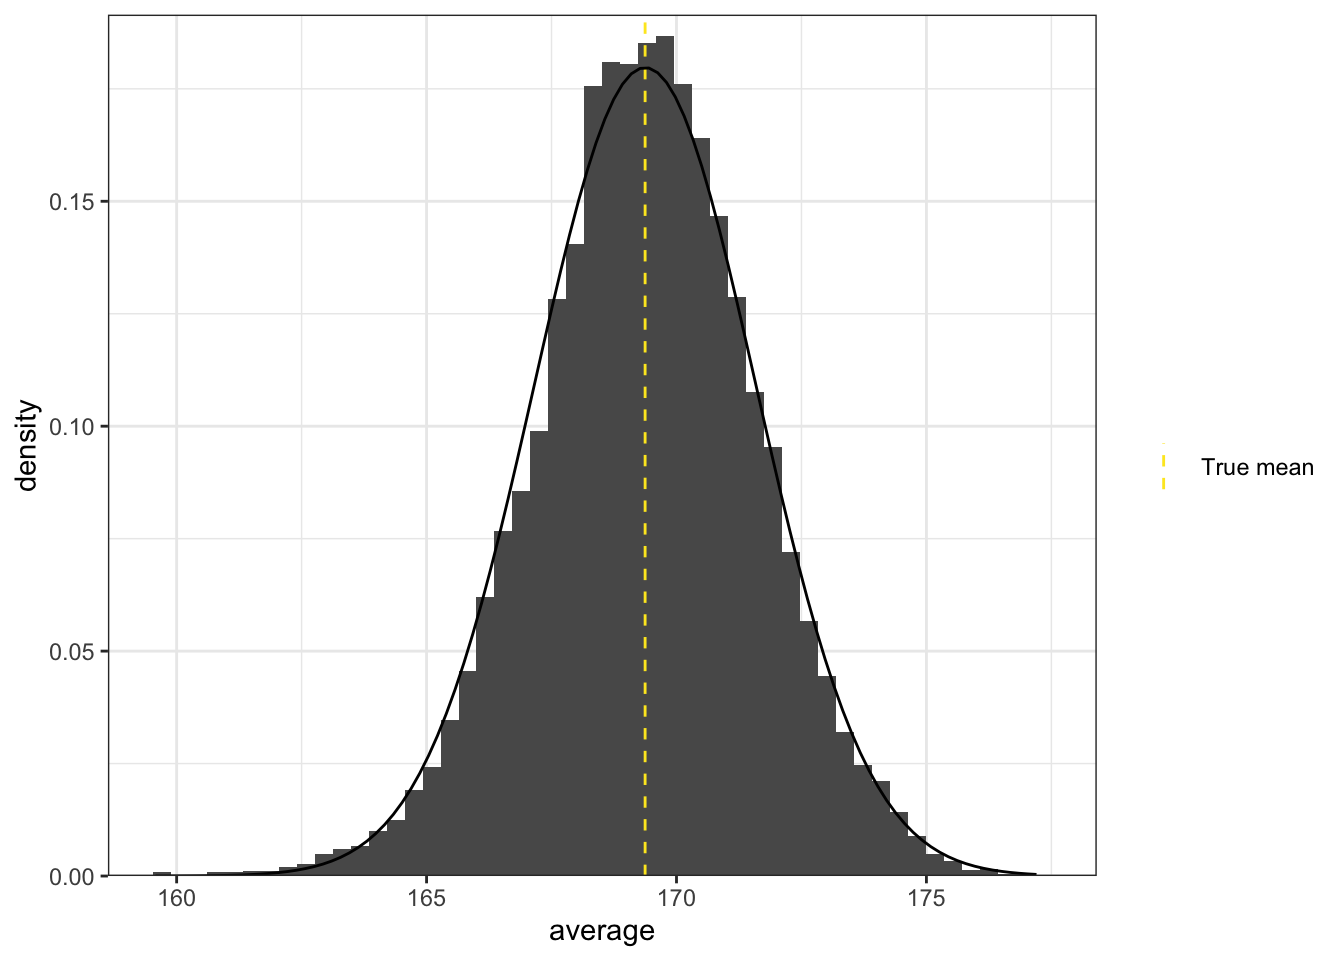
\includegraphics{783_biostats_files/figure-latex/unnamed-chunk-68-1.pdf}

\hypertarget{estimating-mean-depression-score-1}{%
\subsubsection*{Estimating Mean Depression Score}\label{estimating-mean-depression-score-1}}
\addcontentsline{toc}{subsubsection}{Estimating Mean Depression Score}

We argued above that the fact that the average heights follow a normal distribution isn't all that surprising. But we also saw that the mean depression score actually looks like something that is normally distributed. Well, again, we can use the CLT to calculate the normal distribution it should follow.

The mean depression score in the entire population is 3.49, and the variance of the depression scores in the population is 16.55. So, the average depression score of our samples (that have sample size 50), should follow a normal distribution with mean 3.49 and variance 0.331.

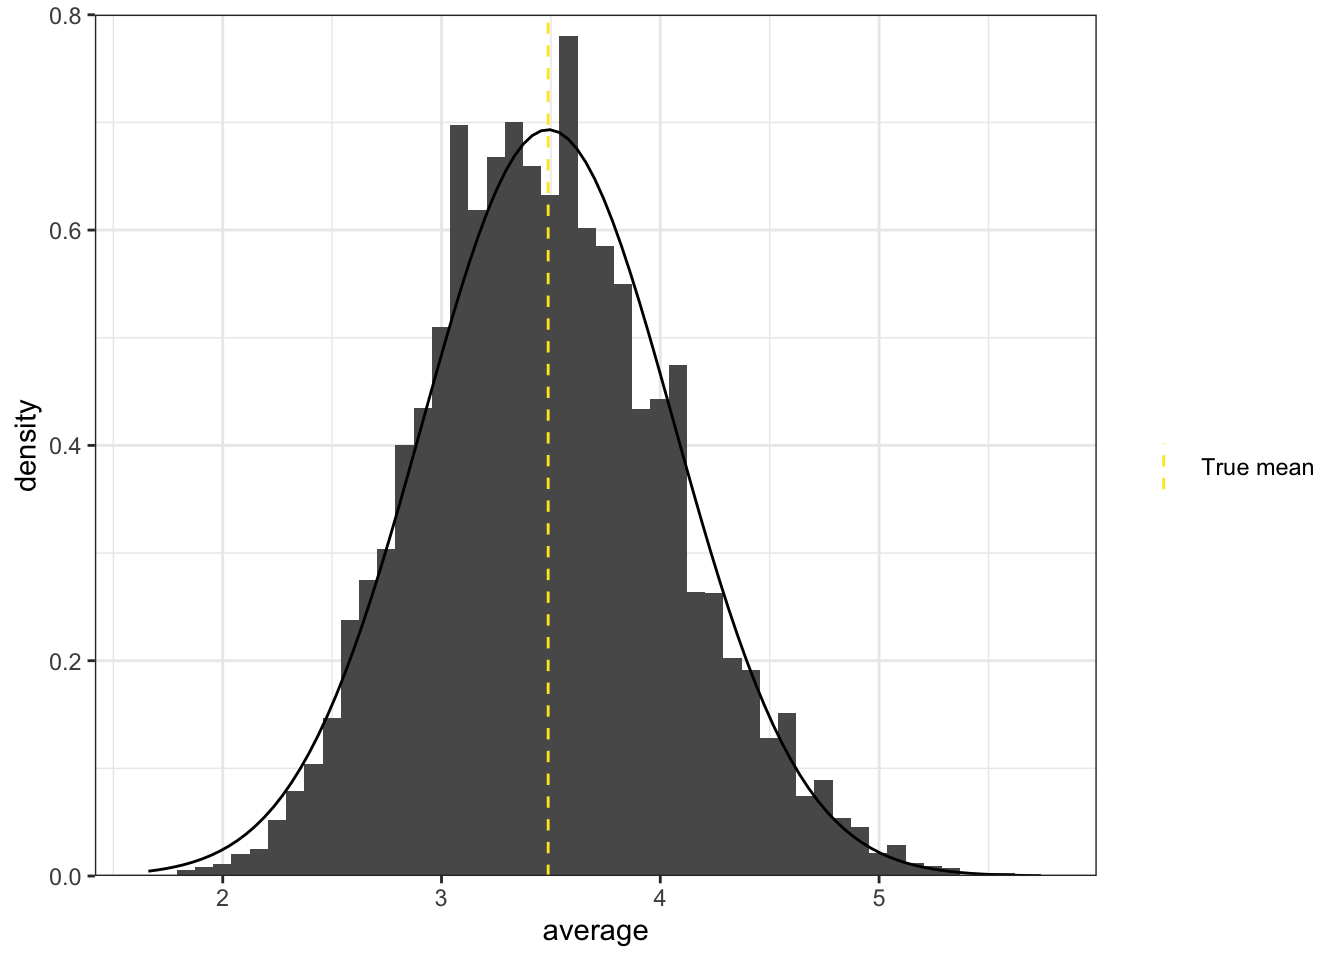
\includegraphics{783_biostats_files/figure-latex/unnamed-chunk-69-1.pdf}

Again, pretty spot on!

\hypertarget{estimating-proportion-of-men-1}{%
\subsubsection*{Estimating Proportion of Men}\label{estimating-proportion-of-men-1}}
\addcontentsline{toc}{subsubsection}{Estimating Proportion of Men}

For completion, we consider the last example from above to which the CLT applies. When estimating the proportion of men in the population, the sample proportion also follows a normal distribution, and again we can calculate the mean and variance of that distribution.

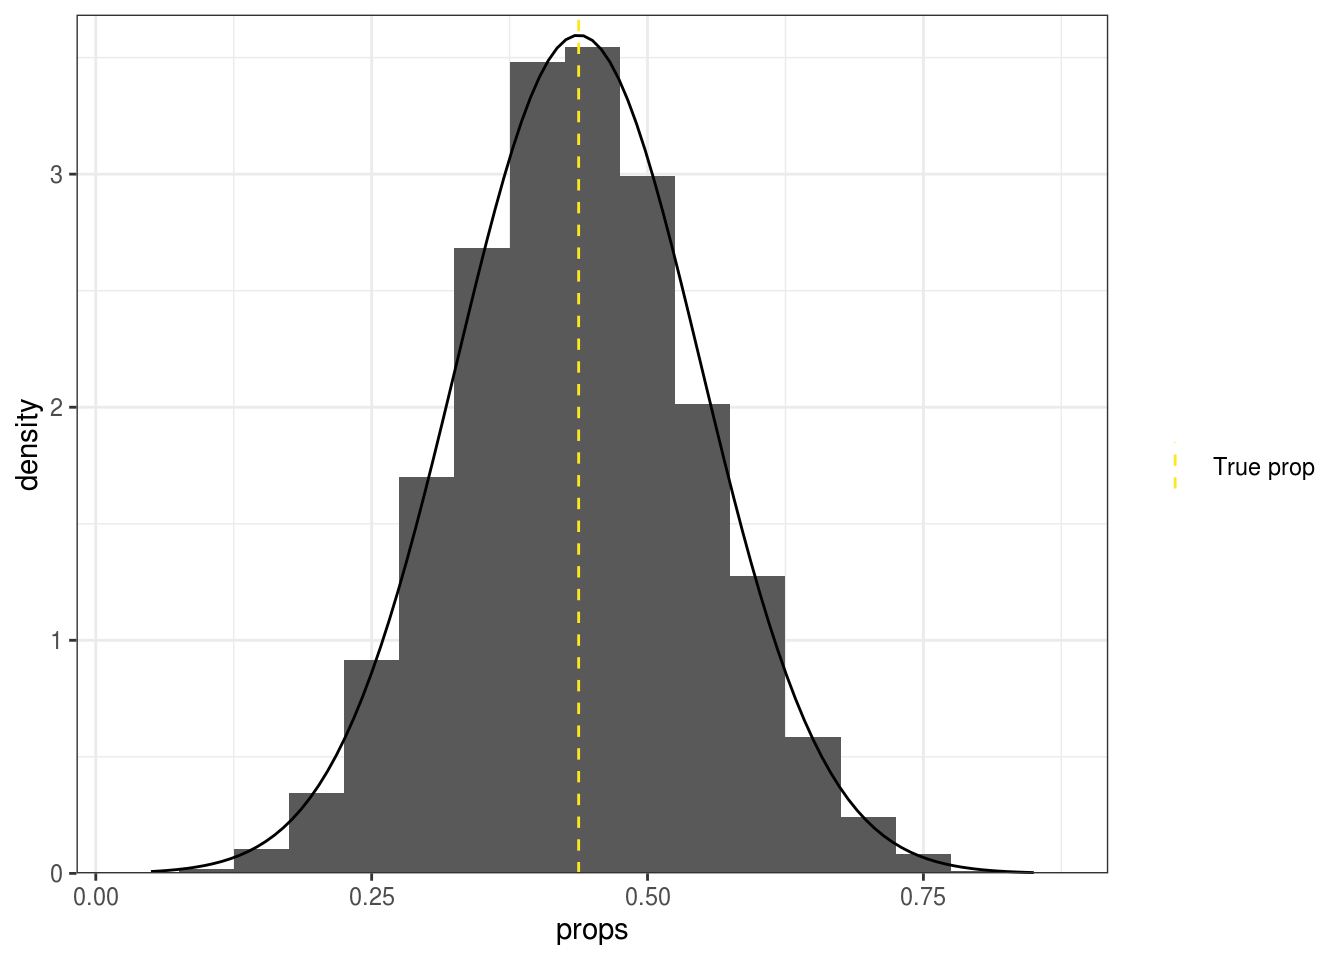
\includegraphics{783_biostats_files/figure-latex/unnamed-chunk-70-1.pdf}

\hypertarget{even-more-examples-for-the-curious}{%
\subsubsection*{Even more examples for the curious}\label{even-more-examples-for-the-curious}}
\addcontentsline{toc}{subsubsection}{Even more examples for the curious}

To explore more, you can spend a few minutes \href{https://rtrane.shinyapps.io/CLT_2/}{here}. Data can be simulated from a number of different distribution, or you can upload a data set (such as the FHS data set).

\hypertarget{part-statistical-hypothesis-testing}{%
\part{Statistical Hypothesis Testing}\label{part-statistical-hypothesis-testing}}

\hypertarget{introduction-to-statistical-hypothesis-testing}{%
\chapter{Introduction to Statistical Hypothesis Testing}\label{introduction-to-statistical-hypothesis-testing}}

Quick recap: some population is identified in which we're interested in a particular feature (mean BMI, prevalence of disease, etc.). The only way to find the Truth\textsuperscript{TM} is to examine every single individual in the population, and calculate the value of interest. Unfortunately, this is not possible, so instead we get a representative sample from the general population. In this sample, we can calculate anything we'd like. The question is then, how can we use this sample to say something about the Truth\textsuperscript{TM}?

As an illustrative example, say we are interested in testing a hypothesis that the true mean value in a population is 6 against an alternative hypothesis that the true mean value in the population is not 6. In statistical jargon, we say we're testing the null hypothesis \(H_0: \mu = 6\) against the alternative \(H_A: \mu \neq 6\). To do so, we look at our sample, and estimate the population mean with the sample average. In the previous section, we saw that the Central Limit Theorem guarantees that the sample average will be ``pretty close'' to the true population mean (as long as \(n\) is ``large enough''), and so using the sample average to try to say something about the true population mean seems like a good ide.

The question we seek to answer is IF the true population mean is indeed 6, would it be reasonable to see the sample average we see? It seems fair to say that if the sample average we see is very close to 6, then it's reasonable for us to believe that the true population mean is in fact 6, while if our sample average is far from 6, it would be reasonable to dispute the idea that 6 is the true population mean. So, the question then becomes, when is our average far from 6, and in particular, how far from 6 does it have to be before we don't believe that 6 is indeed the true population mean?

Obviously, the real answer is ``it depends, and is very subjective''. We will try to remove the first part, and bring the subjective part of the answer to a scale that everyone can relate to.

Consider the two visualization of our hypothesized population mean and sample average depicted in figure \ref{fig:comp1}. Would you say the sample average is far from the hypothesized value on the figure to the left? What about the one on the right?

\begin{figure}
\centering
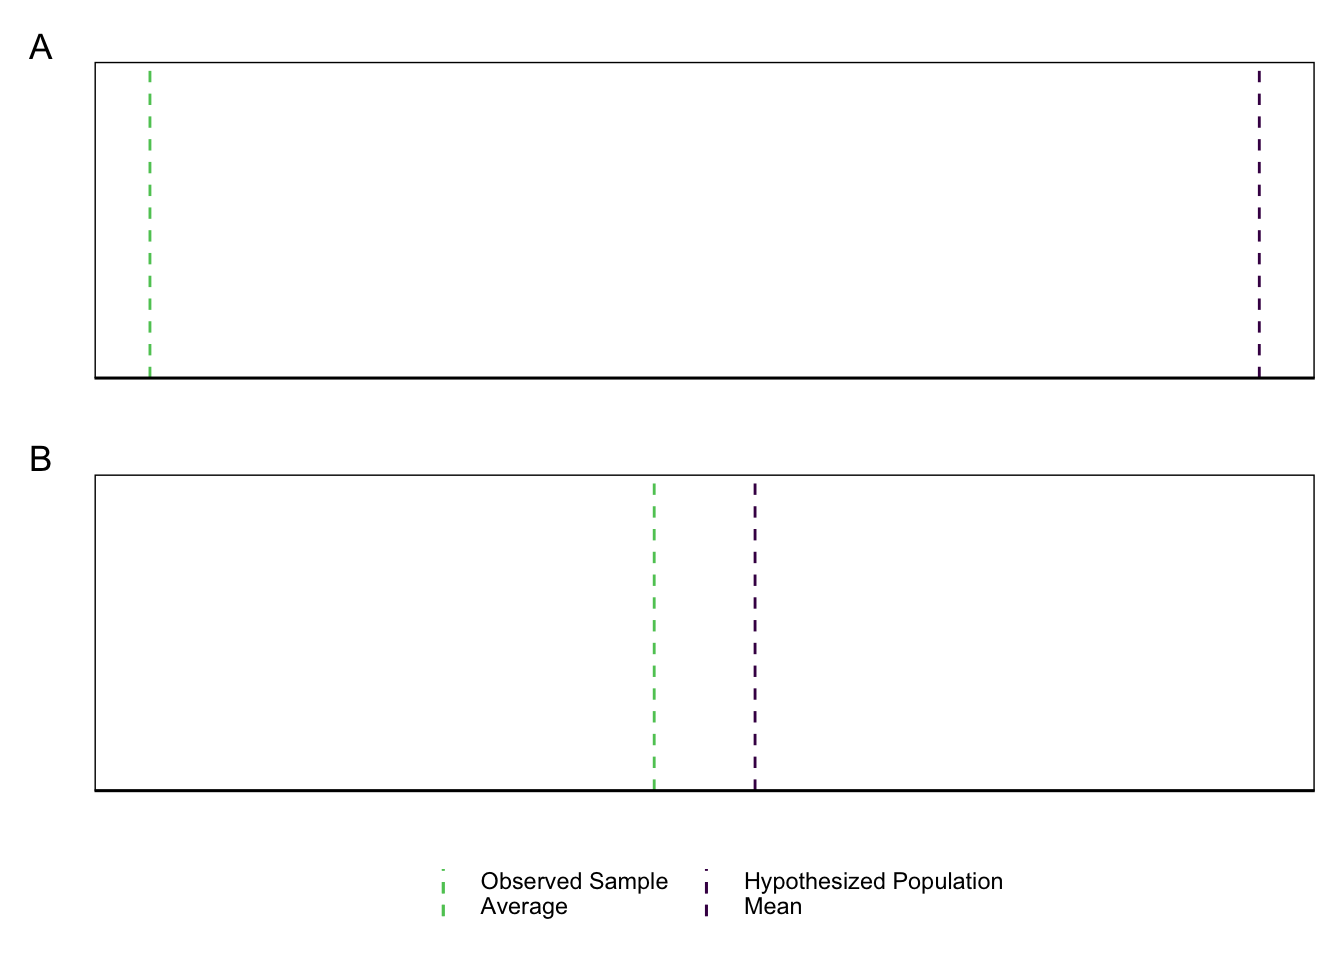
\includegraphics{783_biostats_files/figure-latex/comp1-1.pdf}
\caption{\label{fig:comp1}Are the two lines far about?}
\end{figure}

We can't really tell. We need some more context. So what if we knew the difference between the two? Are they far apart?

\begin{figure}
\centering
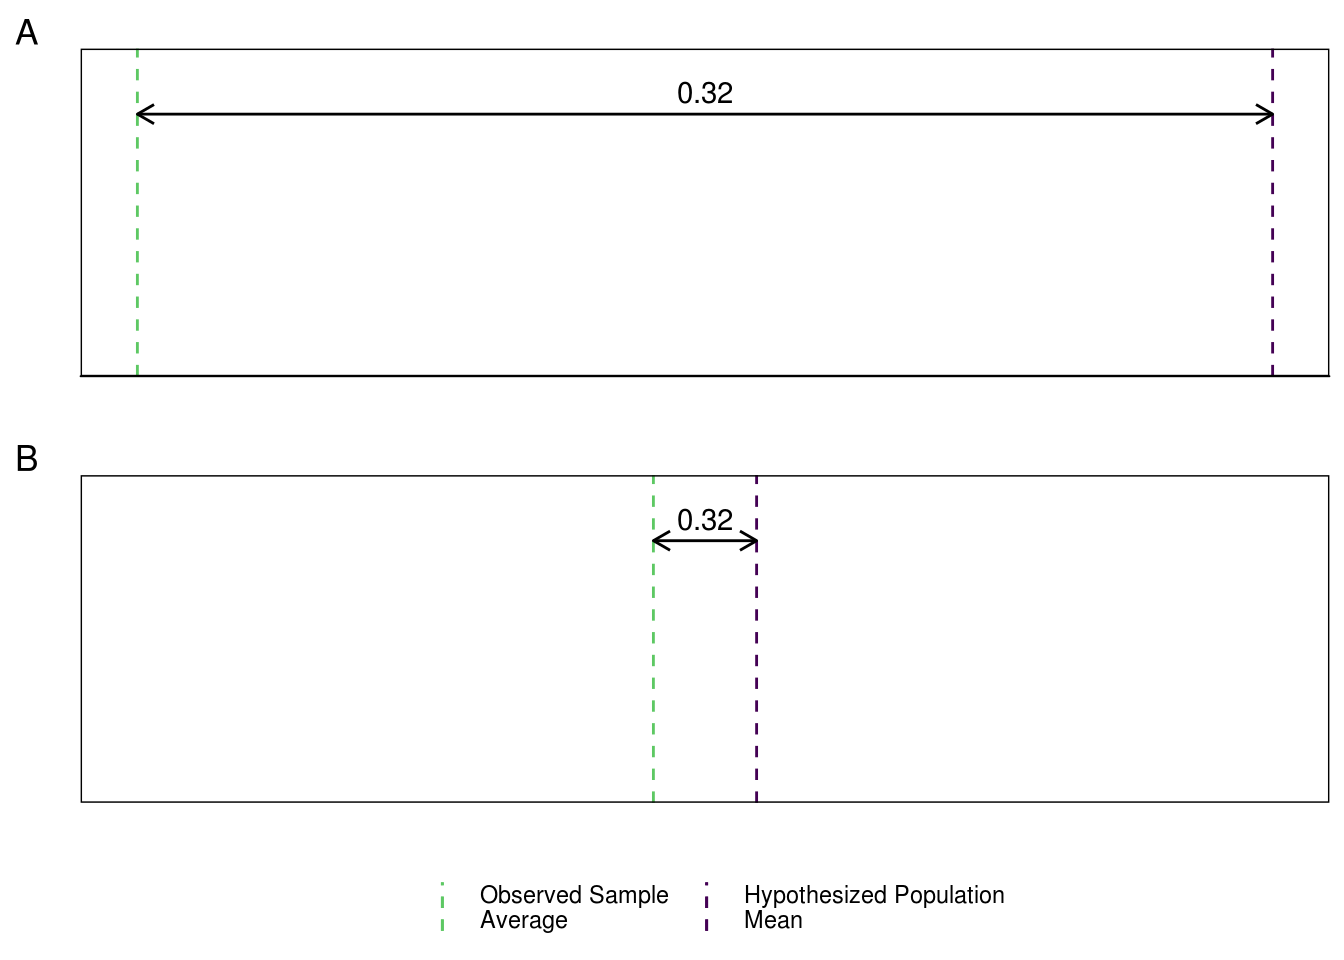
\includegraphics{783_biostats_files/figure-latex/comp2-1.pdf}
\caption{\label{fig:comp2}Adding the actual difference doesn't help much.}
\end{figure}

Still impossible to say, but what if we add a scale to it all? The difference between \(1000000\) and \(1000001\) is basically negligible, while the difference between \(0.0001\) and \(1.0001\) seems huge, even though both differences are \(1\). So we add the scale.

\begin{figure}
\centering
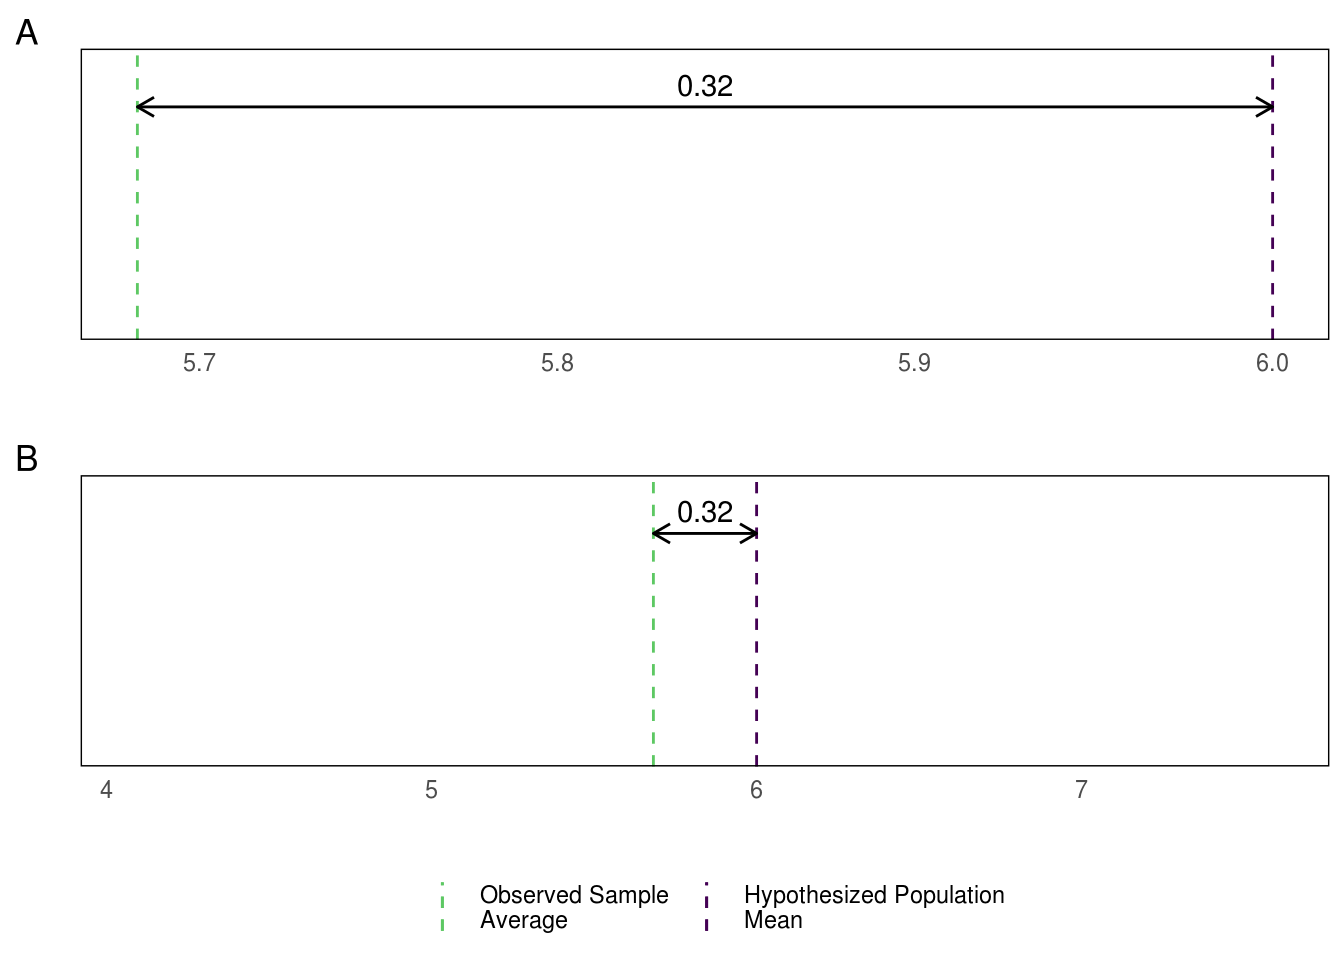
\includegraphics{783_biostats_files/figure-latex/comp3-1.pdf}
\caption{\label{fig:comp3}With a scale, it is a bit better.}
\end{figure}

This solved one problem. You can't mislead me anymore (at least not as much) simply by changing the scale (i.e.~zooming in/out), since I can now compare the difference to the absolute values of the two to get some sort of idea of the size of the difference. However, it is still kind of hard to say if the sample average is far from the hypothesized mean or not.

Now, consider the two figures below. Same dotted lines, but the sample average is computed from two different samples (both samples consist of 10 observations, and they both have the same average).

\begin{figure}
\centering
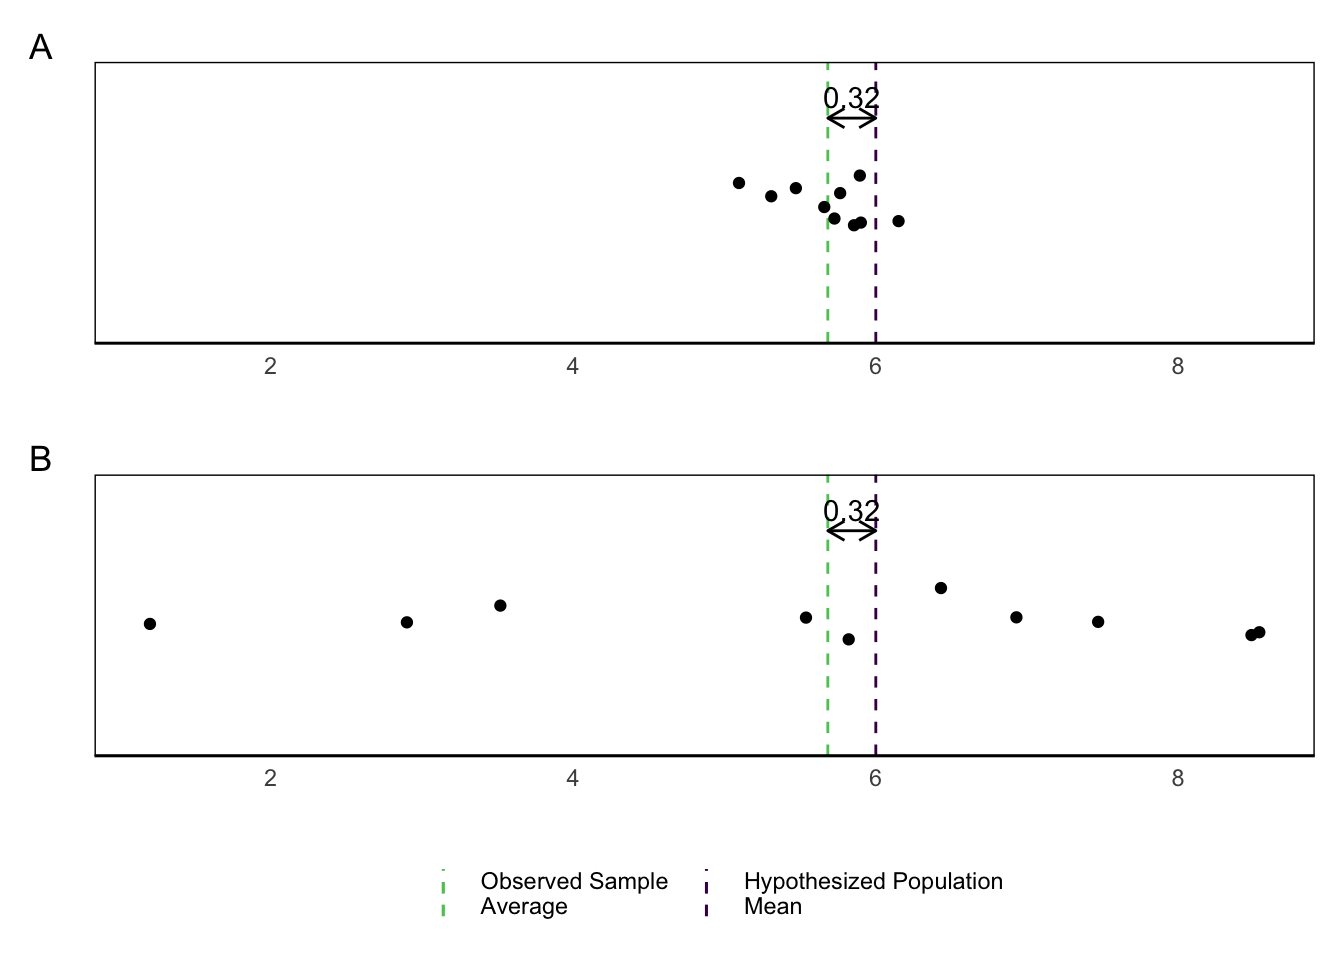
\includegraphics{783_biostats_files/figure-latex/comp4-1.pdf}
\caption{\label{fig:comp4}Actually seeing the data makes everything clear.}
\end{figure}

Now I all of a sudden feel much more informed. In the case of the sample in subfigure A, I would definitely argue that the sample average is far from the hypothesized population mean -- the average is found in a sample where only one observation is larger than the hypothesized mean. On the other hand, the sample in subfigure B indicates to me that the two lines aren't that different at all.

When looking at the two figures, I subconsciously compare the difference between the sample average and the hypothesized population mean to the variation of the data. If the difference is big compared to the variation of the data, I think the difference between the sample average and the hypothesized population mean is large, and therefore the hypothesized population mean doesn't seem to plausibly be the correct population mean. If the difference is small compared to the variation of the data, I would probably think this is simply due to randomness from the sampling rather than due to the true population mean being different from the hypothesized population mean. So, in subfigure A above I would probably conclude that the hypothesis is incorrect, and therfore reject it, while in subfigure B I would probably NOT come to the same conclusion.

The next question is then when the difference is ``large enough''\footnote{note: this could be in either the positive or negative direction!} relative to the variation that we no longer believe the hypothesized population mean to be the Truth\textsuperscript{TM}. As an example, consider the figures below. Here the variation is the same, but the actual sample averages are different. When is the separation between the data and the hypothesized mean so large that we no longer think it can be attributed to randomness from sampling, and more likely is due to a wrong hypothesis?

\begin{figure}
\centering
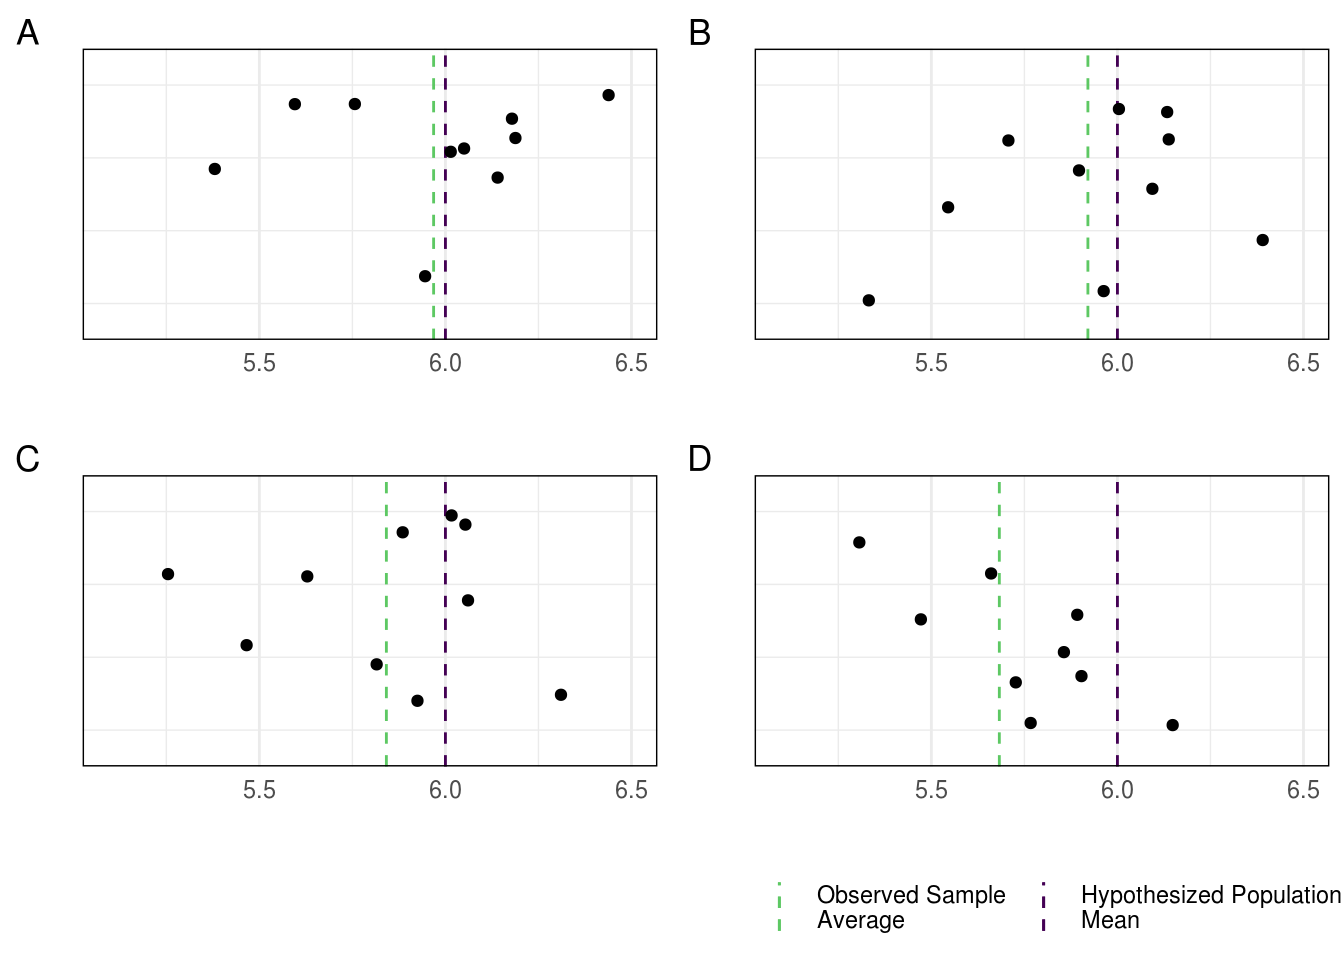
\includegraphics{783_biostats_files/figure-latex/comp5-1.pdf}
\caption{\label{fig:comp5}When is the data far enough from the hypothesized mean?}
\end{figure}

To answer this question, first we need to characterize the difference we can expect from random sampling. Remember, random sampling is governed by probabilities, which in turn are characterized by distributions. If we can find the distribution the quantity we're interested in would have \emph{IF} the hypothesized mean is the true population mean, then we can say something about what kind of difference we would expect from random sampling \emph{IF} the hypothesized mean is in fact the true population mean.

Recall that the \protect\hyperlink{CLT}{Central Limit Theorem} tells us exactly what the distribution of an average is: it states that (when \(n\) is ``large enough''), the average follows a normal distribution centered around the true population mean with variance \(\sigma^2\) over \(n\). I.e. \(\bar{X} \sim N\left(\mu, \frac{\sigma^2}{n}\right)\). So if we pretend \(\mu_0\) is the true population mean, and that we actually know \(\sigma^2\) (which we never do, but let's pretend\ldots), then we know the distribution of \(\bar{X}\)! We can use this to quantify how far from \(\mu_0\) the observed value of \(\bar{X}\) actually is. This is done in terms of the probability of observing something that's even further away. If there's little chance of observing something further away from \(\mu_0\) than what we observe in our sample, then what we observe must be pretty far away. On the other hand, if the probability of observing something further away from \(\mu_0\) than what we observe is rather large, then what we observe must be pretty close to \(\mu_0\).

Compare the observed values of the sample average to the distribution it would follow \emph{IF} the true population mean is indeed \(\mu_0\) on the figure below.

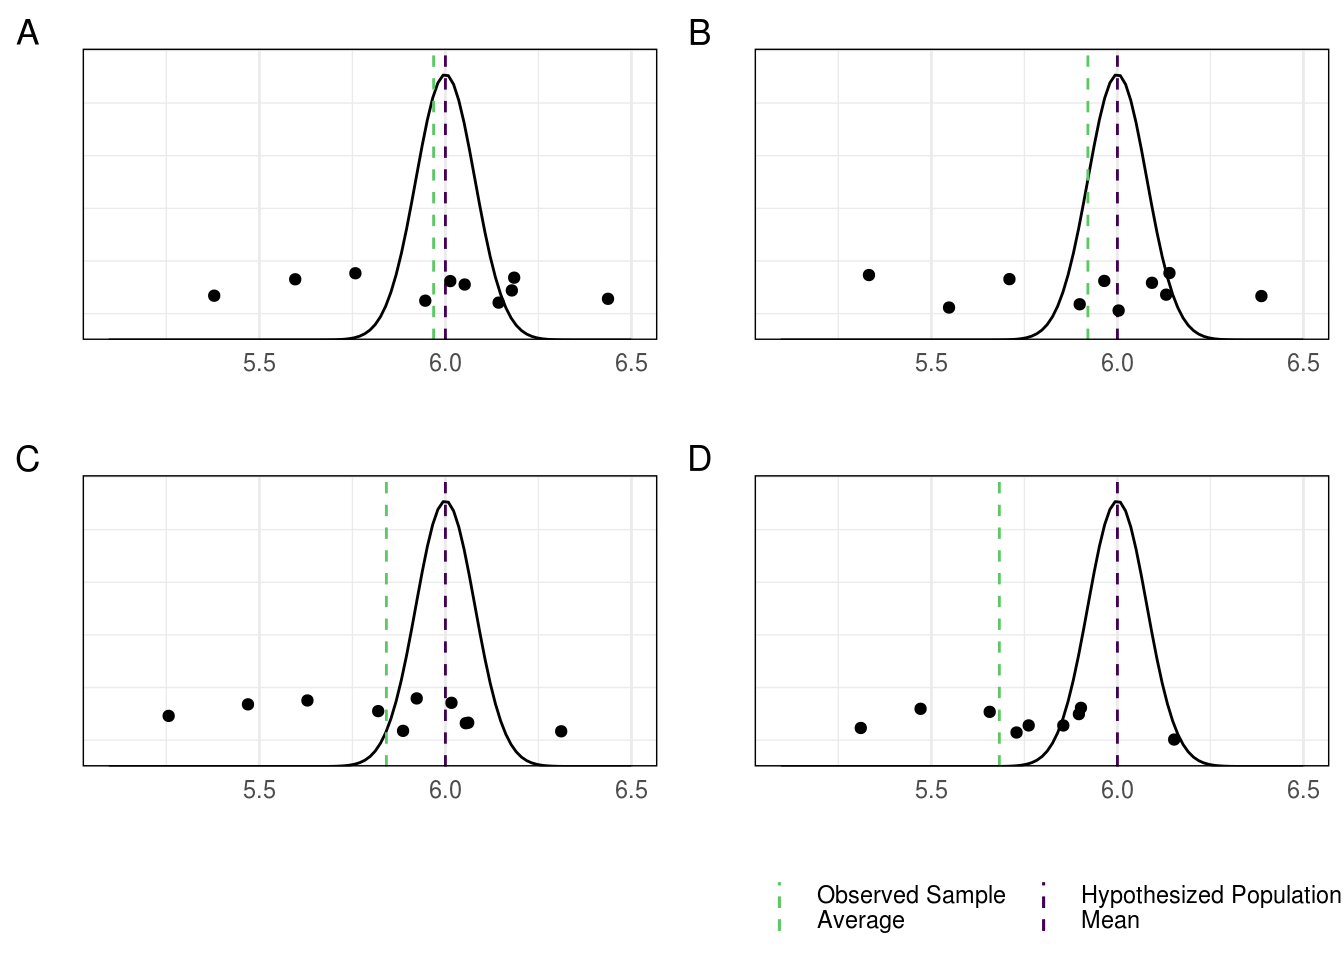
\includegraphics{783_biostats_files/figure-latex/comp-to-dist-1.pdf}

In each of the four cases, what is the probability of observing something ``further away''? First, we need to define what is ``further away''. There's basically three options: further to the left, further to the right, or either. Which realm we're in depends on our alternative hypothesis. The alternative hypothesis basically decides which direction we care about. If the alternative is \(H_A: \mu < \mu_0\) we only care about being ``further to the left''. If the alternative is \(H_A: \mu > \mu_0\) we only care about being ``further to the right''. If the alternative is \(H_A: \mu \neq \mu_0\), we care about both.

In the second paragraph in this section, we decided on using \(H_A: \mu \neq \mu_0\) as the alternative. Recall we find probabilities for continuous random variables as the area under the curve. So the probability of observing something ``further away'', if the true population mean is indeed \(\mu_0\), would be the shaded areas below.\footnote{To see this, ask yourself: ``which is further away from 2: 3 or -1?'' This is why we consider both sides of the hypothesized population mean.}

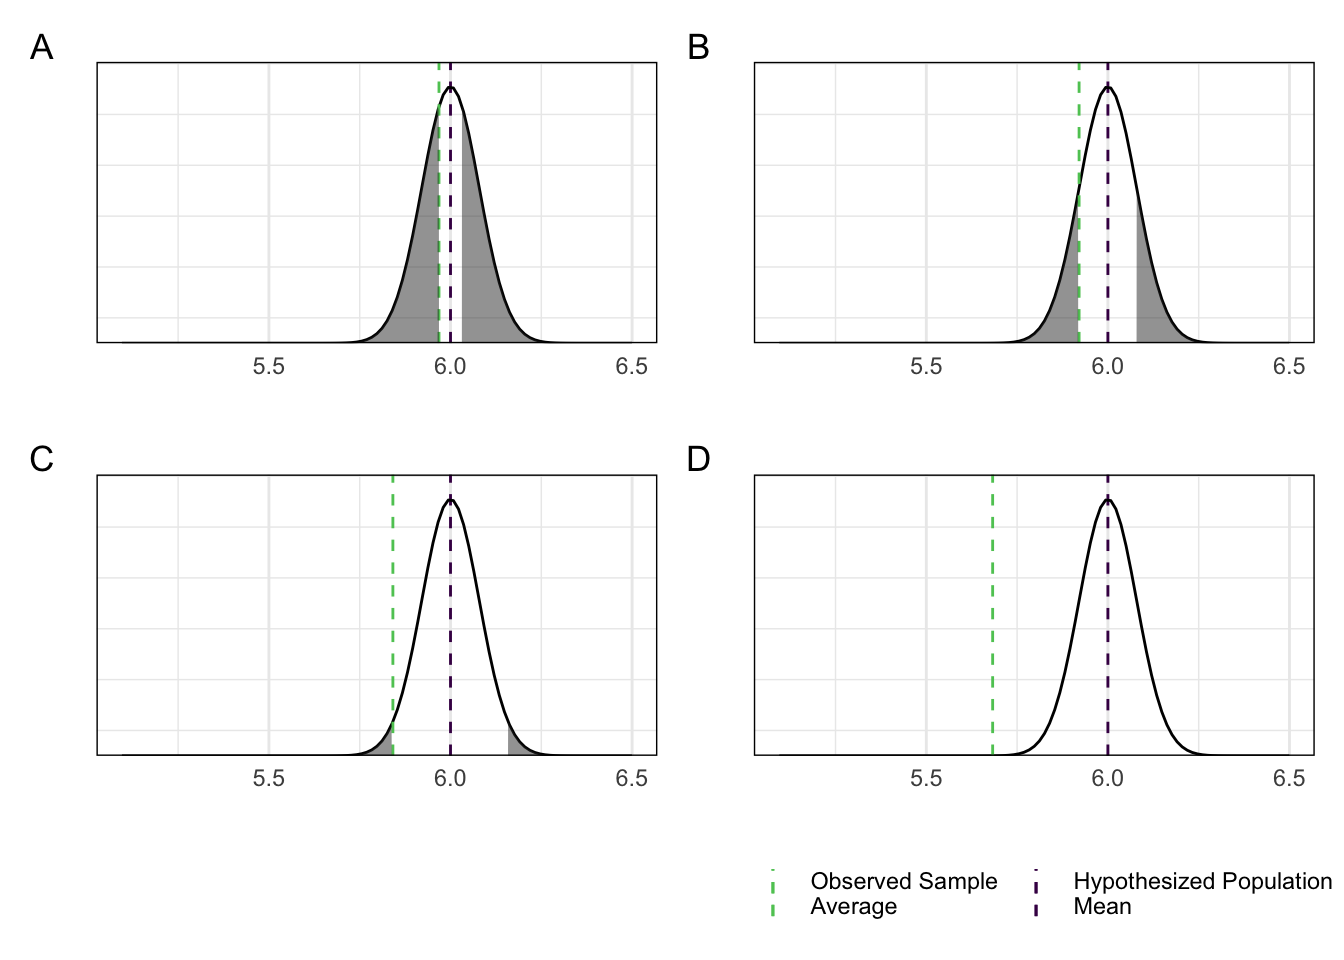
\includegraphics{783_biostats_files/figure-latex/unnamed-chunk-74-1.pdf}

So now we have a metric for being ``far away'' that is completely independent of the scale of the data! In all cases, the probability of being ``further away'' is between 0 and 1. There's still a subjective question left to answer: when is the probability of being ``further away'' small enough that we conclude what we observed is indeed far away? The scientific community has to a large extent decided that 0.05 is a good cut-off point. Note that this is completely arbitrary, and any cut-off could be used! It comes down to how harsh you want to be: a smaller cut-off needs ``more evidence''.

In the above discussion, we pivoted from looking at the data (the difference between the average and the hypothesized mean compared to the variation in the data) to look at the probability of observing an average that is farther away from the hypothesized mean than what we have observed in the sample, \emph{IF} the hypothesized mean is indeed the true population mean. We could only do this because we assumed that we actually know the true standard deviation. In this case, the Central Limit Theorem gives us the distribution of \(\bar{X}\). Specifically, it tells us that \(\bar{X} \sim N\left(\mu_0, \frac{\sigma^2}{n}\right)\) (again, assuming \(\mu_0\) is the true population mean). In this case, we know from section \ref{lin-comb-normals} that \(\frac{\bar{X} - \mu_0}{\sigma/\sqrt{n}} = \frac{\bar{X} - E(\bar{X})}{\text{SD}(\bar{X})} \sim N(0,1)\) (take a normally distributed random variable, subtract its mean, and divide by the standard deviation). If we look at this quantity, it is \emph{exactly} what we started out with: it is the difference between the average and the hypothesized population mean relative to the variation of the data! (Recall, \(\sigma\) is the standard deviation of the data.) So not only can we actually find the distribution this quantity follows (\emph{IF} the hypothesized mean is truly the population mean), it is also a metric for the thing we actually want to measure! In general, such a quantity is called a \emph{test statistic}. It is the statistic (i.e.~function of the data) that we will use to perform our test. This particular quantity is called the \emph{z-score} or \emph{z-statistic}, and will be the backbone of many of the hypothesis tests we will see in this section.

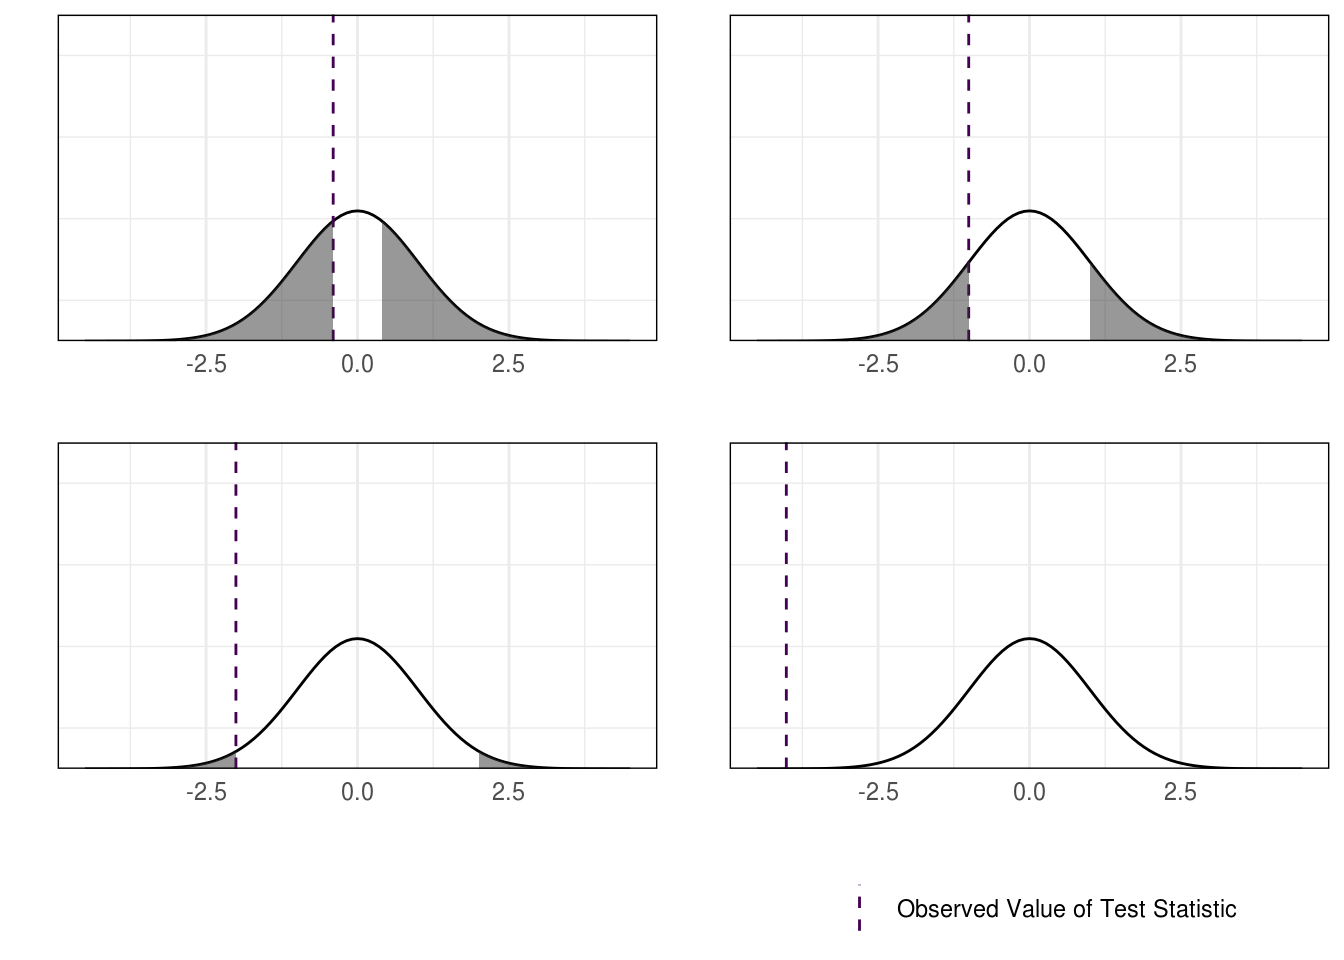
\includegraphics{783_biostats_files/figure-latex/unnamed-chunk-75-1.pdf}

\hypertarget{strategy-overview-the-lingo}{%
\section{Strategy Overview \& The Lingo}\label{strategy-overview-the-lingo}}

The general strategy for testing a hypothesis is as follows:

\begin{itemize}
\tightlist
\item
  define your null and alternative hypotheses, \(H_0\) and \(H_A\)

  \begin{itemize}
  \tightlist
  \item
    the null hypothesis is ALWAYS going to be the simple hypothesis. Above, \(H_0: \mu = \mu_0\).
  \item
    the alternative can often be one of three: \(H_A: \mu < \mu_0\), \(H_A: \mu > \mu_0\), or \(H_A: \mu \neq \mu_0\). The latter is more common. The two inequalities often used when trying to determine superiority/inferiority of a new drug/treatment
  \end{itemize}
\item
  define you \emph{significance level} \(\alpha\)

  \begin{itemize}
  \tightlist
  \item
    this is the cut-off value for the probability of observing something ``further away''
  \end{itemize}
\item
  find a \emph{test statistic} that somehow quantifies the ``distance'' from your data to your hypothesis

  \begin{itemize}
  \tightlist
  \item
    in the example above, we settled on \(\frac{\bar{X} - \mu_0}{\sigma/\sqrt{n}}\)
  \end{itemize}
\item
  make sure you can determine the distribution of your test statistic \emph{ASSUMING} the hypothesis is true

  \begin{itemize}
  \tightlist
  \item
    this is referred to as the \emph{null distribution}, since it is the distribution \emph{IF} the null hypothesis is true
  \item
    above, we saw that \(\frac{\bar{X} - \mu_0}{\sigma/\sqrt{n}} \sim N(0,1)\) \emph{IF} \(\mu_0\) is indeed the true population mean
  \end{itemize}
\item
  calculate the observed value of your test statistic

  \begin{itemize}
  \tightlist
  \item
    above, you would take the observed data, calculate the average, then find \(\frac{\bar{x} - 6}{\sigma/\sqrt{1}}\)
  \end{itemize}
\item
  compare the observed value of your test statistic to its distribution, and compute the probability of observing something ``further away'' from the hypothesis

  \begin{itemize}
  \tightlist
  \item
    what consitutes ``further away'' depends on your alternative hypothesis
  \end{itemize}
\end{itemize}

\hypertarget{when-we-dont-know-sigma2}{%
\section{\texorpdfstring{When we don't know \(\sigma^2\)}{When we don't know \textbackslash sigma\^{}2}}\label{when-we-dont-know-sigma2}}

Everything above was assuming that \(\sigma^2\) is known, i.e.~we know the \emph{true population} variance of the measurements we're interested in. In the cases where we do NOT know the true standard deviation (spoiler alert: that's all of them!), and we have to \emph{estimate} it from the data, we run into a bit of trouble. The distribution of \(\bar{X}\) is no longer known to us, and \(\frac{\bar{X} - \mu_0}{\sigma/\sqrt{n}}\) isn't really a relevant quantity anymore -- since we do not know \(\sigma\), we cannot calculate the observed value of the test statistic! All is not lost, though. Generally two scenarios when we do not know \(\sigma^2\): we have to estimate it, or it follows from the null hypothesis.

Cases where it follows from the null hypothesis are the ``simplest'' cases. We'll see examples of this in the coming section. When it does not follow from the null hypothesis, we have to estimate it. In the example above, we would ``simply'' estimate \(\sigma^2\) from the data as \(s^2 = \frac{1}{n-1}\sum_{i=1}^n (x_i - \bar{x})^2\). It turns out, when we simply plug this into the z-statistic, we get a new statistic that is really nice. This is called the \emph{t-statistic}, and it follows a \protect\hyperlink{t-distribution}{t-distribution} with \(n-1\) degrees of freedom.

\hypertarget{appendix-appendix}{%
\appendix}


\hypertarget{lecture-slides}{%
\chapter{Lecture Slides}\label{lecture-slides}}

\textbf{Lecture 1 (9/12)} \href{./lectures/lecture01/lec01_slides.html}{slides}

\textbf{Lecture 2 (9/26)} \href{./lectures/lecture02/lec02_slides.html}{slides}

\textbf{Lecture 3 (10/1)} \href{./lectures/lecture03/lec03_slides.html}{slides}

\textbf{Lecture 4 (10/3)} \href{./lectures/lecture04/lec04_slides.html}{slides}

\textbf{Lecture 5 (10/8)} \href{./lectures/lecture05/lec05_slides.html}{slides}

\hypertarget{references}{%
\chapter*{References}\label{references}}
\addcontentsline{toc}{chapter}{References}

\bibliography{refs.bib}


\end{document}
